\chapter{Experiments}\label{chap:experiments}

In this chapter we describe the experiments we performed on song preprocessing methods chosen in Chapters \ref{chap:lyrics_methods} and \ref{chap:audio_methods}. This includes describing every method's input, training (if there was any) and output (meaning the vector-encoded representations for each song in the SD). All this is presented in Sections \ref{sec:text_experiments}, \ref{sec:simple_audio_experiments} and \ref{sec:deep_audio_experiments}. Another thing we did not cover yet and will be presented here, in Section \ref{sec:similarity_metrics}, is describing how the different vector representations will be aggregated into a definition of similarity.

In Section \ref{sec:evaluation} we acquaint the reader with evaluation methods, the reasons we decided to use them and the evaluation results for each method. The results are first presented separately for each method (or a group of closely related methods) in Sections \ref{sec:text_results}, \ref{sec:simple_audio_resutls} and \ref{sec:deep_audio_results}, and then summarized and interpreted in Section \ref{sec:discussion} where various graphs and tables illustrating the prominent or interesting trends and tendencies can be found. Before all this however, we start with stating, what the expected outcomes were initially.

\section{Expectations}\label{sec:expectations}

Even before reading any literature, we made two main predictions: 
\begin{itemize}
    \item \textbf{First:} Audio-based methods will perform better than text-based methods.
    \item \textbf{Second:} More advanced methods will outperform simpler machine learning methods.
\end{itemize} 
By more advanced methods we mean methods that were invented more recently, are more computationally expensive and/or have a more complicated mathematical idea behind them. 

The first prediction was mostly based on the intuition, that audio contains more information about a song than the lyrics and it is also what people care about more when listening to music, both of which makes it more relevant for song encoding. 

The second prediction was also based on intuition and later supported by reading into this topic. Most of the papers we studied (meaning those in Sections \ref{sec:audio_related_work} and \ref{sec:text_related_work}) were describing neural networks performing audio or text-based recommendation or classification. Their results were then compared to simpler algorithms which they mostly outperformed. 

\section{Experimentation protocol}
Every method was trained on either lyrical or audio data of all 16,594 songs from the SD dataset.
For each method (except of raw audio methods which do not need any), we created a model. In addition, we created a matrix --- the \textit{Representation matrix}, denoted as  $R_m$ where $m$ stands for a particular method ---  after training the method's model. Each $R_m$ has the shape of ($16594$ x $l(v_m) $) where $l(v_m)$ is the length of the song vector representation for method $m$. Row $R_{m_{i,*}}$ contains the representation of song $s_i$ from the SD dataset using method $m$. 

We also calculated a \textit{Distance matrix} denoted as $D_m$ for every method. The shape of the $D_m$ is ($16594 $ x $ 16594$) and it is the same regardless of the method. On position $D_{m_{i,j}}$ is the similarity of $R_{m_{i,*}}$ and $R_{m_{j,*}}$. We talk more about similarity in Section \ref{sec:similarity_metrics}. \\

To make things easier for the rest of the thesis we now present all the methods that were tested and introduce a nomenclature. There are 3 different
parts each method name has --- the name of the main algorithm, the name of the input and the length of the output vector. Every method can be uniquely 
identified by a combination of these three parts. Where there is only one or
two parts necessary to uniquely identify the method, we omit those parts which are surplus. \\
The tested methods are:
\renewcommand\labelitemii{\textperiodcentered}
\begin{itemize}
     \item \textbf{Tf-idf} which stands for the Tf-idf method. \\
        Training is described in \ref{ssec:TF_idf_experiments} and the results in \ref{ssec:tf_idf_results}.
    \item \textbf{PCA\_Tf-idf} which stands for PCA with Tf-idf vectors as input. \\
    Training is described in \ref{ssec:PCA_on_tf_idf_experiments} and the results in \ref{ssec:pca_tf-idf_results}.
    \item \textbf{W2V} which represents the Word2Vec method. \\
        The training is described in \ref{ssec:w2v_experiments} and the results in \ref{ssec:w2v_results}.
    \item \textbf{SOM\_PCA\_Tf-idf} and \textbf{SOM\_W2V} which stand for the SOM network with PCA\_Tf-idf vectors as input and the SOM network with W2V vectors as input. \\
            Training is described in \ref{ssec:som_experiments} and the results in \ref{ssec:som_results}.
    \item \textbf{Raw mels} which are raw mel-spectrograms. \\
             Training described in \ref{ssec:raw_mels_experiments} and the results in \ref{ssec:mel_results}.
    \item \textbf{Raw MFCCs} which are raw MFCCs. \\
        Training is described in \ref{ssec:raw_mfccs_experiments} and the results in \ref{ssec:raw_mfccs_results}
    \item \textbf{PCA\_spec\_1106} and \textbf{PCA\_spec\_320} which stand for PCA with spectrograms as input and output lengths of 1,106 for the first method and 320 for the second method. \\
        Training is described in \ref{ssec:PCA_spec_experiments} and the results in \ref{ssec:pca_spec_results}.
    \item \textbf{PCA\_mel\_5715} and \textbf{PCA\_mel\_320} which stand for the PCA with mel-spectrograms as input and the output length of 5,715 for the first method and 320 for the second method. \\
        Training is described in \ref{ssec:pca_mel_experiments} and the results in \ref{ssec:pca_mel_results}.
    \item \textbf{GRU\_spec\_20400} and \textbf{GRU\_spec\_5712} which stand for an autoencoder with GRU layers and spectrogram input. The output vectors have length 20,400 for the first method and 5,712 for the second method. \\
    The architecture is described in \ref{ssec:nn_architectures}, training is described in \ref{ssec:GRU_spec_experiments} and the results in \ref{ssec:gru_spec_results}.
    \item \textbf{LSTM\_spec\_20400} and \textbf{LSTM\_spec\_5712} which stand for an autoencoder with LSTM layers and spectrogram input. \\
        The architecture is described in \ref{ssec:nn_architectures}, training is described in \ref{ssec:LSTM_spec_experiments} and the results in \ref{ssec:LSTM_spec_results}.
    \item \textbf{GRU\_mel} which stands for an autoencoder with GRU layers and mel- spectrogram input. \\
        The architecture is described in \ref{ssec:nn_architectures}, training is described in \ref{ssec:GRU_LSTM_mel_experiments} and the results in \ref{ssec:GRU_LSTM_mel_results}.
    \item \textbf{LSTM\_mel} which stands for an autoencoder with LSTM layers and mel- spectrogram input. \\
    The architecture is described in \ref{ssec:nn_architectures}, training is described in \ref{ssec:GRU_LSTM_mel_experiments} and the results in \ref{ssec:GRU_LSTM_mel_results}.
    \item \textbf{GRU\_MFCC} which stands for an autoencoder network with GRU layers and MFCCs as input. \\
        The architecture is described in \ref{ssec:nn_architectures}, training is described in \ref{ssec:GRU_LSTM_MFCC_experiments} and the results in \ref{ssec:GRU_LSTM_MFCC_results}.
    \item \textbf{LSTM\_MFCC} which stands for an autoencoder with LSTM layers and MFCCs as input. \\
        The architecture is described in \ref{ssec:nn_architectures}, training is described in \ref{ssec:GRU_LSTM_MFCC_experiments} and the results in \ref{ssec:GRU_LSTM_MFCC_results}.

    
\end{itemize}

\section{Text method experiments}\label{sec:text_experiments}

\subsection{Tf-idf experiments}\label{ssec:TF_idf_experiments}

\subsubsection{Input}
The lyrics of each song from SD were stripped of all punctuation characters as well as apostrophes and converted into a single string. All lyric-strings were appended into a list of strings which formed the training dataset.
\subsubsection{Training}
The training dataset was given to the \texttt{fit\_transform} method as a parameter. The method was called on an instance of \texttt{TFidfVectorizer} from Python's \texttt{sklearn} package. The results were saved into the $R_{Tf-idf}$. The \texttt{TFidfVectorizer} instance was saved as the model to be potentially used in the proposed web application. 

\subsubsection{Output}
The song representations were vectors of length 40,165. They contained a lot of zeros so it was possible to store them as \textit{sparse vectors}. Sparse vectors however, are more difficult to operate with and therefore we also converted them into dense vectors.

\subsection{PCA on Tf-idf}\label{ssec:PCA_on_tf_idf_experiments}

Because simple Tf-idf yielded good results we wanted to implement it. The long vectors posed a problem to our web application though. It is sometimes necessary in the application to calculate the distance between a newly added song and all the songs that are already in the database and this calculation is more complex for longer vectors. To reduce the complexity of this task but still use Tf-idf we decided to try to reduce the dimensions of the vectors using PCA.

\subsubsection{Input}
As input, we provided the Tf-idf vectors for songs from SD to the PCA which we acquired as described \ref{ssec:TF_idf_experiments}. We did not normalize them.

\subsubsection{Training}
We first trained a PCA from Python's \texttt{sklearn.decomposition.PCA} without any dimensionality reduction. We then chose a space were the explained variance ratio was equal to 90\%. This space had 4,457 dimensions. Knowing this, we trained a new PCA instance with 4,457 components which reduced our Tf-idf vector's length from 40,165 to 4,457 and saved it as the model.

\subsubsection{Output}
The output were vectors of length 4457 and were saved to the $R_{PCA\_Tf-idf}$.

\subsection{Word2Vec experiments}\label{ssec:w2v_experiments}

\subsubsection{Input}
The input for the W2V model was the same as for the Tf-idf method.

\subsubsection{Training}
In the case of Word2Vec, we did not perform any training. Instead, we used the a subset of the pre-trained W2V model from Google\footnote{https://code.google.com/archive/p/word2vec/} containing 200,000 most common words which cover all meaningful words in the song lyrics we have. Most common means, that they appeared most in their training documents. If there was a word in a song that was not in the subset it was ignored. 

\subsubsection{Output}
Because the Google model takes always just one word as input and returns its vector of fixed length 300, we had to put the word vectors together into one song-representation vector. We chose a basic approach where we averaged all the word vectors into one final song vector. The song vector's position $i$ contained the average over the values of word vectors' position $i$. This approach yielded a vector of length 300 which is significantly lower than the Tf-idf vector.\\

\subsection{SOM experiments}\label{ssec:som_experiments}

\subsubsection{Input}
We tried the W2V vectors from \ref{ssec:w2v_experiments} as input for the self organizing map, mainly because of their length and also because we were hoping, that the SOM could improve the results of the W2V method. We also tried to train the SOM on the output vectors of the PCA\_Tf-idf method. We did not try the raw Tf-idf vectors as they are longer and it would prolong training significantly. Also, it makes sense to use PCA\_Tf-idf because it yielded better results than raw Tf-idf.

\subsubsection{Training}
We used a python library called \texttt{minisom} \cite{Vettigli2019} to create the self organizing maps. We build a map with a grid size $5*|SD|$ and the number of iterations was also 5 times the size of SD. We saved a model after each multiple of 16,594 iterations and interestingly, the representations did not change after 33,187 iterations (which is 2*16,594). It was also necessary to normalize the input vectors and set learning rate to 0.2. Otherwise the songs formed 3 to 5 large clusters on the grid placing thousands of songs on the same coordinate. 

\subsubsection{Output}
The output representation for each song was a vector of length two. It is possible to display the songs on a 2D map which we also did and it can be seen in Figure \ref{fig:som_map}. 

\section{Simple audio method experiments}\label{sec:simple_audio_experiments}

\subsection{Audio preparation}\label{ssec:audio_prep}

In order to encode audios of songs, we first needed to define some kind of standard audio-form to make the audio information suitable for the machine learning methods that we are testing in this section and the next. We decided to extract chunks of the same duration from all songs, so the input vectors for each category (spectrograms, mel-spectrograms and mfccs) are also of the same length within each category. Since all songs have different lengths and one complete 3.5 minute long song results in a spectrogram of size 5,214x2,206 which when flattened is a vector of length 11,502,084 we decided to extract only 15 second excerpts from each song to create spectrograms, mel-spectrograms and MFCCs from those. We took 5 seconds between the 15th and 20th second, 5 seconds starting in the middle of the song and 5 seconds starting 15 seconds before the end. We did not start at the beginning and at the end because in some songs, there is silence or applause or some talking before the actual song starts or after it ends. \\

It was also necessary to decide on some parameters for spectrogram, mel-spectrogram and MFCC extractions such as window width, window overlap and the number of mel-frequency bands. As stated previously, our neural networks were inspired by \cite{inproceedings_RNNs} where they also performed parameter optimisation for the mel-spectrograms which they used as input for neural networks. We decided to use the reported parameters to create the spectrograms, mel-spectrograms in this thesis. We use spectrograms, mel-spectrograms and MFCCs as input for not only neural networks but also the PCA.

The resulting choices were following. We set window width $w$ to 0.2 and window overlap $w_o$ to 0.5$w$ = 0.1. For mel-spectrograms it is also necessary to choose mel-frequency bands which were set to 320 because in the findings from \cite{inproceedings_RNNs}, the performance of neural networks did not increase for values higher than 320. For MFCCs we decided to set the number of coefficients to 320 which is the same as the number of Mel- frequency bands.

With these parameters, the shape of an extracted spectrogram was (408 x 2206) which is a vector of lenght 900,048 when flattened. A mel-spectrogram matrix had the shape of (408 x 320) which when flattened is 130,560 and the MFCC matrix had the shape of (646 x 128) which when flattened is a vector of length 82,688.

We used Python's \texttt{librosa} library \cite{brian_mcfee_2019_2564164} to cut songs into the 15 second excerpts which we then stored the in .wav files. We used methods \texttt{librosa.core.stft} to generate spectrograms \texttt{librosa.feature.mel\_spectrogram} to generate mel-spectrograms and for the MFCC coefficients we used \texttt{librosa.feature.mfcc} all of which received the 15 second audio excerpt from the .wav file loaded using \texttt{librosa.core.load} as a parameter. These functions return a matrix of shape ($m$ x $n$) where $m$ is the number of timestamps and $n$ the number of features. The reason why the MFCC matrix has a different number of timestamps than spectrograms and mel-spectrograms for the same length of audio is, that we only set the number of MFCCs in the \texttt{librosa.core.mfcc} function but left the window width and window overlap default.

\subsection{Raw Mel-spectrograms}\label{ssec:raw_mels_experiments}
The mel-spectrograms were created from the 15 second long audios described in \ref{ssec:audio_prep}. Extracting spectrograms respectively mel-spectrograms does not require any training. It a is mathematical procedure explained in \ref{ssec:mel_spectrograms_intro}. 

As mentioned in the previous section, the mel-spectrograms we got after transforming a 15 second long audio with 320 mel-frequencies bands were matrices of size (408 x 320) which when flattened turned into vectors of size 130,560. This turned out to be too long to implement in our application, however, we still tested this method and the results are in Subsection \ref{ssec:mel_results}. 

\subsection{Raw MFCCs}\label{ssec:raw_mfccs_experiments}
The 15 second audios of all songs from SD were given as parameters into the \texttt{librosa.feature.mfcc} method one by one with parameters defined in \ref{ssec:audio_prep}. Training was not necessary since acquiring mel-frequency cepstral coefficient is a matter of Fourier Transformations and is explained in Subsection  \ref{ssec:mfcc_intro}. The resulting MFCC matrix for one song from SD had the shape of (646 x 128). When flattened we got a vector of length 82,866. That turned out to be too long for practical use in the application. Nevertheless we tested this method and the results can be found in Subsection \ref{ssec:raw_mfccs_results}.

\subsection{PCA with spectrograms}\label{ssec:PCA_spec_experiments}

\subsubsection{Input}
We used spectrograms acquired as described in Section \ref{ssec:spectrogram_intro} as input for the PCA. Because the output of the \texttt{librosa.core.stft} method is a complex matrix, we computed the absolute value of each matrix entry. Afterwards, we flattened the matrix into a single vector and normalized it using a \texttt{MinMaxScaler} from the \texttt{sklearn} Python package. Normalization was very important, without it, the resulting rankings were almost random.

\subsubsection{Training}
Training was a little bit challenging with input vectors of length 900,048. As the whole (16594 x 900048) matrix did not fit into memory at once instead of using \texttt{sklearn.decomposition.PCA} we turned to a PCA with the possibility to be trained in batches. This kind of PCA is also provided by \texttt{skearn} in the \texttt{sklearn.decomposition.incrementalPCA} module. \\ 
Our batch size was 1,106. When we tried to increase it, we got a memory error. This was a little inconvenient because the PCA's the maximum number of components is $min(n\_samples, n\_features)$. In our case, $n\_samples$ was only 1,106 meaning we could get a maximum of 1,106 components which explained about 57\% of the dataset's variance. We saved this incrementalPCA instance with 57\% varince explained as our first model and the method was denoted as PCA\_spec\_1106. 

We then tried to decrease the number of components even more to get vectors of length 320. The lenght was inspired by the number of Mel-frequency bands used when extracting mel-spectrograms. The training was the same as for the PCA\_spec\_1106 but we kept only 320 components and saved the incrementalPCA instance as the model for this method called PCA\_spec\_320.

\subsubsection{Output}
The output vectors for PCA\_spec\_1106 were of length 1,106 and for PCA\_spec\_320 they were of length 320.

\subsection{PCA with mel-spectrograms}\label{ssec:pca_mel_experiments}
\subsubsection{Input}
The input for the PCA\_mel method were mel-spectrograms from \ref{ssec:audio_prep} which were flattened and normalized using a \texttt{MinMaxScaler} from the \texttt{sklearn} Python package.

\subsubsection{Training}
Unlike the spectrograms, mel-spectrograms did fit into memory so we were able to train the PCA on the whole dataset at once. This allowed us determine what number of components explains 90\% of the variance ratio and use it. We found that 90\% of variance is explained by 5,715 components which is what we used to train one model. \\
The results were good, therefore we decided to try reducing the dimension even more to 320 as we did with PCA having spectrograms as input. Like this, we again created two models, the first one is called the PCA\_mel\_5715 the other the PCA\_mel\_320. 

\subsubsection{Output}
The output for the bigger model was a vector of length 5715, for the smaller model, it was a vector of length 320.

\section{Deep audio experiments}\label{sec:deep_audio_experiments}

\subsection{Architecture}\label{ssec:nn_architectures}
Before analysing each of the deep audio methods independently, we will describe the two neural network architectures we used. 

As stated multiple times before, we decided to build the networks based on the \cite{inproceedings_RNNs} paper. We designed the architecture in a way they did with some slight adjustments and extensions. The audio representation learning they performed is displayed in Figure \ref{fig:inspiration_nn}. The first most notable thing is, that their network was designed to classify sounds, not encode songs. However, it consisted of two parts. The first part was an autoencoder and the second part a multi-layer perceptron. The autoencoder was trained in an unsupervised manner and the outputs were then fed into the MLP which did the classification.

We therefore figured, that we can take advantage of the first part of their neural network and discard the MLP. The portion of their procedure that we also performed is marked with the red rectangle which we added to their illustration. The reason why they performed feature fusion in (d) is because they worked with stereo wav files and were putting together the features of the different channels. In our case this was not done as we only had a mono wav files for each song.

\begin{figure}[h]
    \centering
	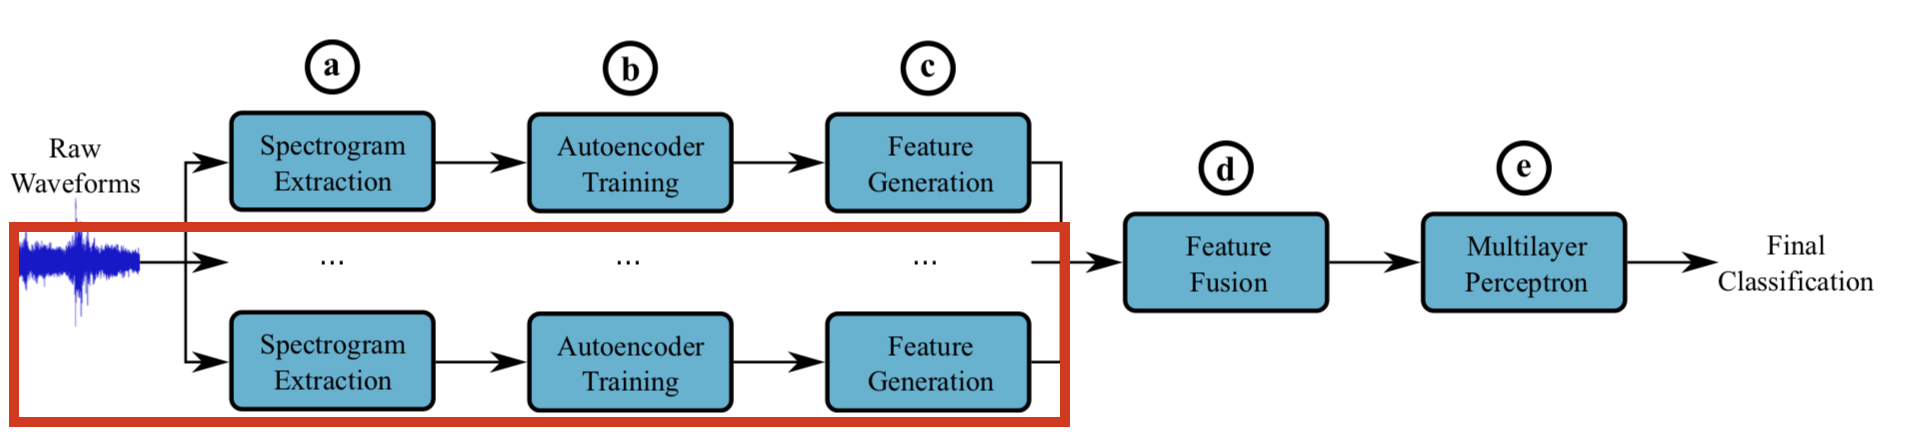
\includegraphics[width=120mm]{./img/inspiration_nn.png}
	\caption{The steps in feature learning from \cite{inproceedings_RNNs} where we also got this diagram from. We added the red rectangle which represents the portion of their procedure that was also (with adjustments) performed by us.}
	\label{fig:inspiration_nn}
\end{figure}

This means, we only used the autoencoder part. Unlike them, instead of using the \texttt{auDeep} library\footnote{https://github.com/auDeep/auDeep} we decided to build the networks with the \texttt{Keras} library \cite{chollet2015keras} as it has a convenient model-creation API for Python. We had also access to GPU computers and \texttt{Keras} (with \texttt{Tensorflow} backend) makes it easy to take advantage of faster training on GPUs. 

We created two architectures. One with two GRU layers for the encoder and one Bidirectional layer for the decoder. This follows the paper. We also decided to create another architecture with LSTM layers instead of GRU layers even though \cite{inproceedings_RNNs} found in their work that the additional complexity did not yield better results. Both architectures can be seen in Figure \ref{fig:nn_architectures}. We decided to use sequence-to-sequence RNNs to encode the vectors.


\begin{figure}[H]
\centering
\begin{minipage}{.45\textwidth}
  \centering
  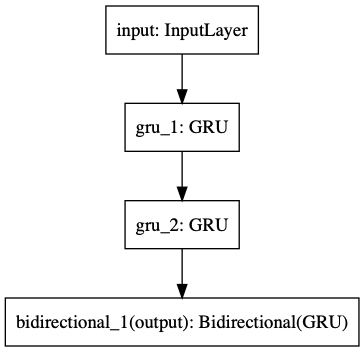
\includegraphics[width=1\linewidth]{./img/gru_architecture.png}
  \caption{The general architecture of GRU neural networks}
  \label{fig:gru_architecture}
\end{minipage}%
 \vspace{1cm}
\begin{minipage}{.45\textwidth}
  \centering
  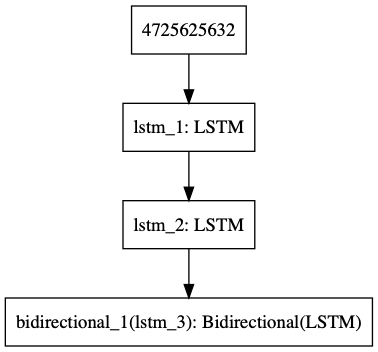
\includegraphics[width=1\linewidth]{./img/lstm_architecture.png}
  \caption{The general architecture of LSTM neural networks}
  \label{fig:lstm_architecture}
\end{minipage}
\end{figure}\label{fig:nn_architectures}

The main motivation behind using LSTMs as well as GRU layers in this thesis was that LSTM layers are specifically suited for sequential data such as audio. GRU layers are a newer, simplified version of LSTMs. We were hoping that the more complex layers could encode audio data into the same dimensions as the GRU networks but help to make the similarities more accurate. 



We used the \textit{mean squared error} as the loss function which is the standard for autoencoder networks. We used the \textit{adam} optimiser, the same as in the \cite{inproceedings_RNNs} paper. We had to decrease the learning rate from 0.001 to 0.0001. Before we did that, the resulting predicted vectors often consisted of just \textit{NaN}s.

\subsection{Inputs and outputs}
Both the GRU and the LSTM network architectures were used to create models with all three kinds of inputs --- the spectrograms, mel-spectrograms and the MFCCs. The inputs were all passed in the form of matrices containing $(n\_features $ x $n\_timestamps)$. GRU as well as LSTM networks take matrices, not just vectors as input. Before training, the input matrices were normalized using the \texttt{MinMaxScaler}. 

One important thing to note here is that we used sequence-to-sequence RNNs so the dimensionality of only the $ n\_features $ and not the $ n\_timestamps $ was reduced. The 15 second audios yielded 408 time stamps and 2206 features for spectrograms which when flattened is a vector of length 900,048 and 408 time stamps and 320 features for mel-spectrograms which is a vector of length 130,560. With MFCCs the number of time stamps was 646 and the number of features 128 which gives us a vector of length 82,688 when flattened. Therefore, we did not attempt a dimensionality reduction as big as with PCA which does not care if a feature is a time stamp or a sample and the output vectors had to be of length at least 408 for autoencoders with spectrograms and mel-spectrograms as input and 646 for autoencoders with mfccs as input. 

The output lengths for the different autoencoders were different depending on the kind of input. The specific values are described in specific method sections along with the reasons for choosing them. Their length is specified as the length of the flattened matrix.

\subsection{GRU network with spectrogram input}\label{ssec:GRU_spec_experiments}

\subsubsection{Training}

We trained two GRU spectrogram networks with variable output vector lengths. We decided to base the output vector's length on the PCA's output vectors that explained 90\% of the variance ratio. For spectrograms however, we only found out that 1,106 explains 57\% of variance. Therefore, we took the information from the mel-spectrogram PCA where 5,715 compnents explain 90\% of variance and did a simple calculation: $$ l(mel\_spec_{transformed})/l(mel\_spec) = l(spec_{transformed})/l(spec) $$ to keep the proportional reduction of spectrograms same as for mel-spectrograms. 

This would mean an output vector length of almost 40,000 which is too much for any practical use in the proposed web application. Because of that we reduced it to 20,400 (408 x 50) which at that point we thought could be potentially used. The fist GRU layer cut the number of features to 100 and the second then to 50.

The second model produced shorter vectors as encodings of songs. The first GRU layer cut the number of features to 28 and the second GRU layer cut it to 14. They were of length 5,712 (we wanted them to be a multiple of 408 so they are not 5,715 as the output vectors of PCA\_mel) when flattened which means, that the output matrix had the shape (408 x 14). This is inspired by the mel-spectrogram PCA reduction as we thought that the neural network could mimic mel-scaling of the spectrogram as well as additional reduction. 

In \cite{inproceedings_RNNs}, they trained their autoencoders for 50 epochs using batch sizes of 64. We found this to be insufficient, especially with the learning rate reduction. For GRU networks with spectrograms we set the number of epochs to 100 and the batch size to 295 (bigger batches did not fit into memory). 

The training losses of these two methods and all other neural network methods are illustrated in Figure \ref{fig:all_model_training}. 

\begin{figure}[h]
    \centering
	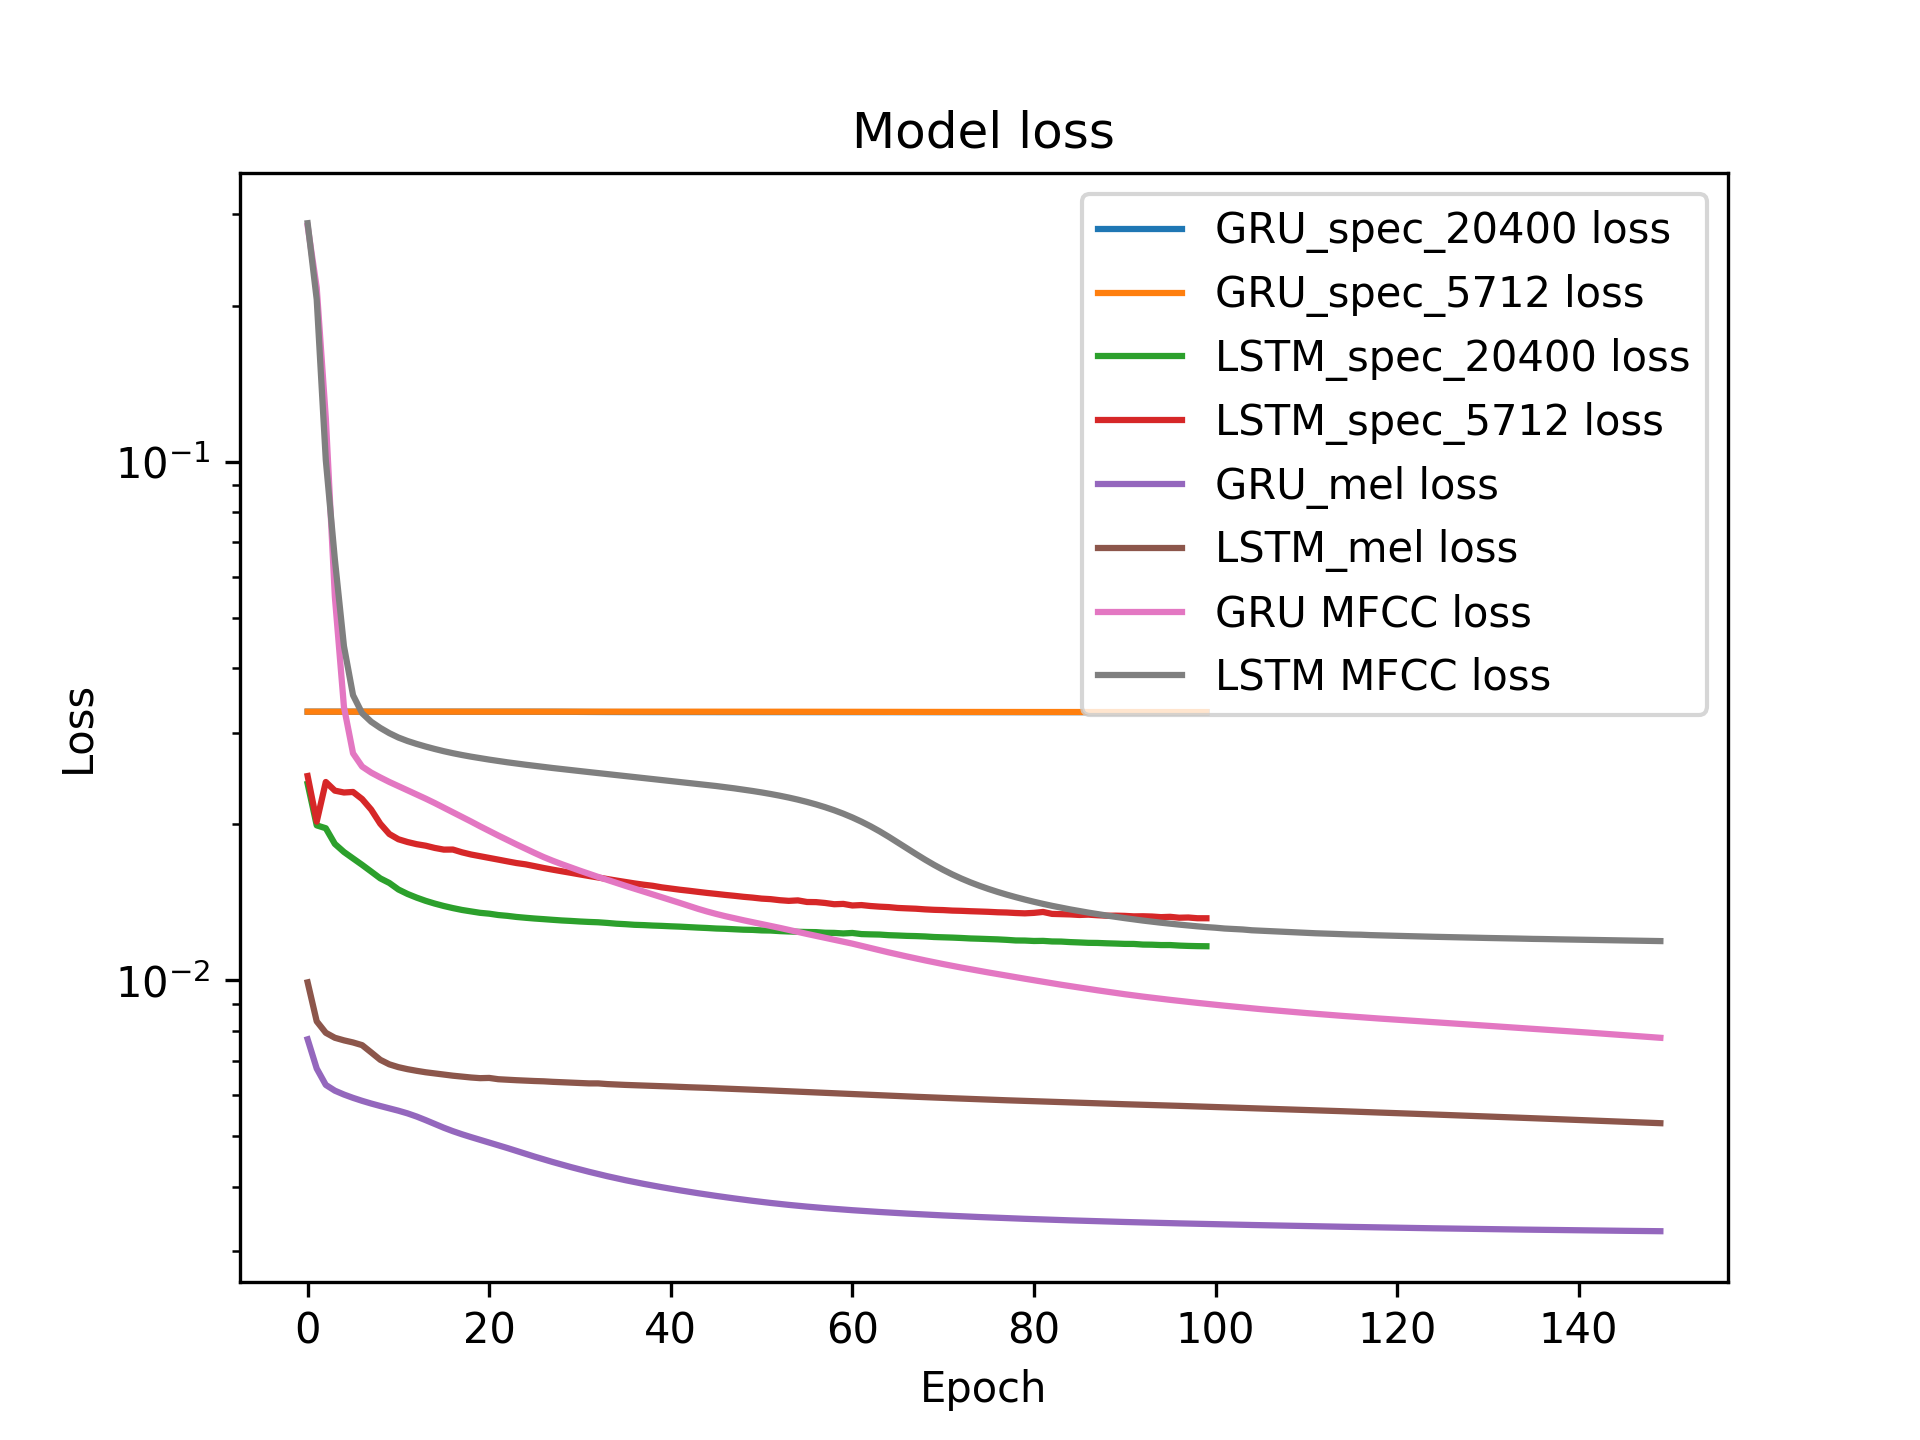
\includegraphics[width=120mm]{./img/all_training_graphs.png}
	\caption[]{The training mean squared error loss values for all the neural network methods that were trained. \\
	\tiny{The blue curve for the GRU\_spec\_20400 is hidden behind the orange curve.}}
	\label{fig:all_model_training}
\end{figure}


\subsection{LSTM network with spectrogram input}\label{ssec:LSTM_spec_experiments}

\subsubsection{Training}
We chose the same training strategy for LSTMs with spectrogram input as we did for the GRU\_spec networks. We created two versions of LSTM models, one is LSMT\_spec\_20400 and the shorter version is LSTM\_spec\_5712. The output lengths are also the same as with GRU\_specs.

\subsection{GRU and LSTM networks with Mel-spectrogram input}\label{ssec:GRU_LSTM_mel_experiments}

\subsubsection{Training}
The GRU\_mel and LSTM\_mel networks were both trained under the same conditions. We trained them on mel-spectrograms for 150 epochs with a batch size of 256. The output length of the encoded song vector was based on keeping 90\% of the variance ratio of the PCA\_mel which was 5,715. The final output length however was not 5,715 but 5,712 (408 x 14) to be divisible by 408. The first GRU/LSTM layer reduced the number of featrues to 28 and the second layer to 14.

We did not attempt any further reductions here partly because as stated before, we were reducing only the number of features with the sequence-to-sequence RNN, so that the minimum length for the encoded vector had to be 408 (which is the number of timestamps). Partly also because vectors of length 5,712 are of acceptable length to be implemented in the proposed web application. 


\subsection{GRU and LSTM networks with MFCC input}\label{ssec:GRU_LSTM_MFCC_experiments}

\subsubsection{Training}
At first we did not plan on using MFCCs as input into neural networks. However because it turned out that raw MFCCs are too long to be used in the proposed application directly we decided to try to reduce their dimension with both the GRU and LSTM network architectures. 

We trained both architectures for 150 epochs and a batch size of 256 which is the same number as for neural networks having mel-spectrograms as input. The output vectors were of length 5,168 when flattened which means the output matrix had the shape of (646 x 8), where the first GRU/LSTM layer cut the number of features to 18 and the second to 8. We were again trying to come close to the number of dimensions that explains 90\% of the variance ratio when using PCA which is 5,715. We chose $646*8$ which is 5,168 rather than $646*9$ which is 5,814 because we favored bigger reduction over proximity to 5,712.

\section{Similarity metrics}\label{sec:similarity_metrics}
As the reader might have noticed, we presented several possible methods which encode a song into a vector. But we still need to define similarity between these vectors. There are many ways of asserting how similar two vectors are, however, we do not consider studying these to be main focus of this thesis. After the initial exploration of this topic, we decided to use the \textbf{cosine similarity metrics} for all the representation methods. 

Although throughout the proposed web application the metric is referred to as distance, it in fact is a similarity measure, meaning, the greater value the more similar two songs are. We use the \texttt{sklearn.metrics.pairwise.cosine\_similarity} method for all the similarity calculations.

\section{Evaluation}\label{sec:evaluation}

\subsection{Desired recommender-system features}
We already touched this in the introduction but it is useful to revise what we want from a good recommendation system and what its most important features are. Let's skip the software part for now as it is further discussed in Chapter \ref{chap:web_app} and focus purely on the quality of recommendations. Probably the most crucial property a recommender system should have is that it should include the relevant items between the first 10 to maybe 50 recommendations. Because it does not really matter if an item the user would like ends up on the 500th or 5,000th position. People rarely go that deep. 

Another thing we want is for the system to be able to improve recommendations when it has more data about a user. In the context of this thesis it means, that we would expect the predictions to be better for users with longer playlists. 

Even though the whole idea of this thesis is to provide variable recommendations, we still want our methods to posses these features to a reasonable extend. Also, since these are the properties other recommendation systems are being evaluated on, we can gain a better understanding of the features our methods share with other recommendation techniques as well as where they differ. 

\subsection{Evaluation measures}\label{ssec:evaluation_measures}
To test the wanted features described in the section above we performed evaluation as follows. 

The UD dataset contains 11,123 playlists that were used for evaluation. We chose to evaluate the tested methods only on playlists of length at least four. For each method, we did a 5-cross-validation where in a validation epoch, every playlists $p_i$ was divided into two parts a training part $p_{i_{train}}$ and a testing part $p_{i_{test}}$ and the values of the evaluation measures below were determined. The playlists were split in an approximately 80:20 ratio. A higher priority was set on the fact that the test part always had to contain at least one entry (meaning that for playlists of length 2, the ratio would be 50:50). \\ \\
The processing of one playlists was performed as follows: 

For each song $ s_k $ from the song dataset SD, the similarity of the whole $p_{i_{train}}$ to $s_k$ which we denote as $ sim(p_i, s_k) $ was calculated as $$ sim(p_i, s_k) =\sum_{s_j\in{p_i{_{train}}}} cos\_sim(s_k, s_j) $$ where $ k \neq j$ and $cos\_sim$ is the cosine similarity. These similarities were then sorted in a descending order and it was determined at what position the songs from $p_{i_{test}} $ came as those are the ones that actually belong to the playlist. 

These positions were then used to calculate multiple evaluation measures to assess how well each algorithm predicts the missing part of a user's playlist. We chose the following evaluation measures:
\begin{itemize}
    \item Recall at 10 (= \textbf{R@10}) defined as the proportion of songs from $p_{i_{test}} $ that placed between the top ten most similar songs.
    \item Recall at 50 (= \textbf{R@50}) defined as the proportion of songs from $p_{i_{test}} $ that placed between the top fifty most similar songs.
    \item Recall at 100 ( = \textbf{R@100} ) defined as the proportion of songs from $p_{i_{test}} $ that placed between the top hundred most similar songs.
    \item Normalized cumulative discounted gain (= \textbf{nCDG}) defined as 
    $${nDCG_{r}} = \frac{DCG_{r}}{IDCG{r}} $$
    where 
    $${DCG_{r}} =\sum_{k=1}^{r}{\frac {rel_{k}}{\log _{2}(k+1)}} $$ 
    is the discounted cumulative gain at position r and 
    $$ {IDCG_{r}} =\sum _{k=1}^{|REL|}{\frac {2^{rel_{k}}-1}{\log _{2}(k+1)}} $$
    is the ideal discounted cumulative gain at r
    where $r$ is the number of songs that had to be predicted, the $rel_k$, meaning relevance, is the same for all songs because all songs in one playlists have the same relevance and $|REL|$ is the length of the list of relevant items (in this case the songs from $p_{i_{test}}$).
    \item Average rank of a song from the $p_{i_{test}}$ set $ \boldsymbol{ (= \overline{rank})} $ which we included to have also an indicator of the overall behaviour, not only the first 100 ranks.

\end{itemize}

The overall evaluation results for a tested method were then taken as its 
average evaluation-measure values over all the playlists over the 5 
cross-validations. In addition we also retrieved the evaluation values for only certain playlist's lengths again by averaging over the 5 cross-validations but selecting only values of playlists of desired lengths.

Moreover, we created one more evaluation technique whose purpose was to visualize the results of a method. It is a graph plotting the distribution of rankings of songs from the test part of each playlists. It is denoted as the \textbf{RDG} (=\textit{rank distribution graph}). The number of songs from $p_{test}$ (which is a union of all songs from all $p_{i_{test}}$) for each individual rank from 1 to 16,594 is summed and divided it by the number of all songs in $p_{test}$. So for example if we had two playlists both with two songs in $p_{test}$ and a method assigned ranks 30 and 2,900 to the $p_{test}$ songs from the first playlist and 2,900 and 4,872 to those from the second playlists, the graph would plot the values 0.25 for rank 30, 0.5 for rank 2,900 and 0.25 for rank 4,872 and 0 for the rest of the ranks. We did this with all playlist lengths included but we also plotted these distributions for chosen playlist lengths separately to see if the predictions improve for longer playlists which we expect from a good recommender system. The x-axis of the \textit{RDG} was log-scaled as we are much more interested in what is going on among the first 100 positions than in what is going on in the middle or towards the end. 
    
After running the evaluation, we noticed from the RDGs that for most of the similarity methods, the positions for songs from $p_{i_{test}} $ where $p_i$ was a short playlist were higher up, than those from long playlists especially for the first three ranks. We concluded that the reason for such behaviour could be, that inside all playlists, there are groups of very similar songs but the groups are rather dissimilar to each other. Songs which are somewhat similar to all groups then cloud the recommendations and take place of songs that are very similar to one group but dissimilar to the other groups.

Because of this, we changed the recommendation method a little bit. We set a threshold for each similarity metrics, and if the similarity between two songs was smaller than this threshold, we set the similarity to 0. This means, that the new similarity function $cos\_sim_t(s_i,s_j)$ is defined as follows:

\[   
cos\_sim_t(s_i,s_j) = 
     \begin{cases}
       \text{$ cos\_sim(s_i,s_j) $} &\quad\text{if $ cos\_sim(s_i,s_j)$} \geq \text{threshold}\\
       \text{$ 0 $} &\quad\text{if $ cos\_sim(s_i,s_j)  < threshold$}\\
     \end{cases}
\]

 The threshold for a method was chosen as the value of the 846,294th biggest element from its $D_m$. 846,294 is $ 51 * |SD| $. The most similar song is always the song itself, so it leaves us with approximately 50 most similar songs for each song. 50 is approximately 0.03\% of 16,594 so we also refer to the threshold as the 0.03\%-threshold throughout this thesis. 
 
The results presented in Sections \ref{sec:text_results}, \ref{sec:simple_audio_resutls} and \ref{sec:deep_audio_results} are all acquired by evaluation of recommendations using the similarity with threshold. If the evaluation of similarity without threshold had better results for a method, it is mentioned in the method's section. 

Another reason to use the threshold-similarity is the fact, that we use the threshold to calculate similarity in the proposed application. Not only because of the better results as we shall see, but also because of the fact, that it dramatically reduces the number of similarities that have to be stored in the database. The 0.03\%-threshold values for various methods are in Table \ref{table:threshold_table}.\\
\begin{table}[h]
\centering

%\renewcommand{\arraystretch}{1.5}
\begin{tabu} to 1.7\textwidth {| c | c | c | c |}
\hline
Tf-idf & W2V & PCA\_Tf-idf & SOM\_W2V \\ 
\hline 
0.2817861171 & 0.956714893 & 0.189907224 & 0.999997393 \\
\hline
\hline

PCA\_mel\_320 & PCA\_mel\_5715 & PCA\_spec\_1106 & PCA\_spec\_320 \\ 
\hline
0.383122074 & 0.189912771 & 0.3368717729 & 0.442181335\\
\hline
\hline

GRU\_spec\_20400 & GRU\_spec\_5712 & LSTM\_spec\_20400 & LSTM\_spec\_5712 \\
\hline
0.999742671 & 0.99999024 & 0.975920383 & 0.981116184 \\
\hline
\hline

GRU\_mel & LSTM\_mel & GRU\_MFCC & LSTM\_MFCC \\
\hline
0.3634592744 & 0.994544642 & 0.953069695 & 0.997860599 \\
\hline
\end{tabu} 
\caption{Table containing the value of the similarity threshold we used. The threshold for a particular method is always below the method's name.}
\label{table:threshold_table}
\end{table}

To give an idea about how the results changed with the threshold, lets take a look at the plot in Figure \ref{fig:absolute_value_comparison}. We plotted the change in the maximum, average and minimum values of our evaluation measures for all playlists and also for different playlist lengths with and without using the threshold for similarity definition. Short playlists in this graph are defined as playlists of lengths 4 to 7 and their evaluation values have an "\_S" appended at the end. Medium playlists are of lengths 8 to 15 and have "\_M" appended. Long playlists are playlists 16 and longer with and "\_L" appended. Although, the minimum values did not improve much, the difference for the maximum and most notably the average values is appreciable. The most crucial remark here is the behaviour of short and long playlists. The results for short playlists did not improve much, especially the maximum values, whereas the results for long playlists improved quite a lot. This is exactly what we anticipated when applying the threshold and also better performance for longer playlists is the desired behaviour for recommender systems.

\begin{figure}[h]
    \centering
	\includegraphics[width=1\linewidth]{./img/mean_min_max_measure_comparison.png}
	\caption{The comparison of absolute max, average and min values for the evaluation measures for recommendation with and without threshold}
	\label{fig:absolute_value_comparison}
\end{figure}

Even with the threshold, we can observe in the \textit{RDG} graphs later on in specific method result sections, that for short playlists, the first one to four ranks are very numerous. For the following ranks however, there is a sharp drop, which does not happen so noticeably with longer playlists. This behaviour inspired us to use the threshold and even though it is less significant after applying it, it is still observable in almost every method.




\section{Text method results}\label{sec:text_results}

As mentioned in Section \ref{sec:evaluation} we calculated each of the five measures (\textit{R@10, R@50, R@100, $ {\overline{rank}} $} and \textit{nGDC} for each playlist and then averaged the values over the whole playlist dataset. Every method section (not only for text methods but also for simple and deep audio methods) contains a table with the five measure averages and a RDG graph. Both are accompanied with a short summary of the most prominent observations.

\subsection{Tf-idf results}\label{ssec:tf_idf_results}

The results of the Tf-idf method place well above average between our methods. This was a bit of a surprise as we did not expect this "simple" method to perform so well compared to others. 

\begin{table}[h]
\centering
\renewcommand{\arraystretch}{1.5}
\begin{tabu} to 1\textwidth {| c || X[c] | X[c] | X[c] | X[c] | X[c] | }
 \hline
 \textbf{method} & \textbf{R@10} & \textbf{R@50} & \textbf{R@100} & \textbf{nGDC} & $ \boldsymbol{\overline{rank}} $ \\
 \hline
 \hline
 Tf-idf & 0.05045 & 0.06187 & 0.06648 & 0.04214 & 7795 \\
 \hline
 PCA on Tf-idf & 0.05417 & 0.0635 & 0.06649 & 0.04371 & 7838 \\
 \hline
\end{tabu} \\
\caption{Table summarizing average Tf-idf and Tf-idf with PCA evaluation measure values averaged over the 5 cross validation that were performed.}
\label{table:1}
\end{table}

When looking at the numbers in Table \ref{table:1} we can see that 5\% of songs that were in our $p_{test}$ set ranked in the top ten, 6.2\% in the top fifty and 6.6\% in the top hundred. The average rank of a song from the $p_{test}$ was 7795 which is quite close to the middle. We also crated an \textit{RDG} as one can see in Figure \ref{fig:tf_idf_distribution}. It appears that according to the distribution, a song is more likely to end up in the first 10-100 songs than it is at the end.

Another thing to notice in \ref{fig:tf_idf_distribution} is that there is a general trend not only for the Tf-idf to rank a lot of songs between the first few but then drop sharply for further ranks for short playlists. Longer playlists seem to drop more steadily.

\begin{figure}[h]
\centering
\begin{minipage}{.45\textwidth}
  \centering
  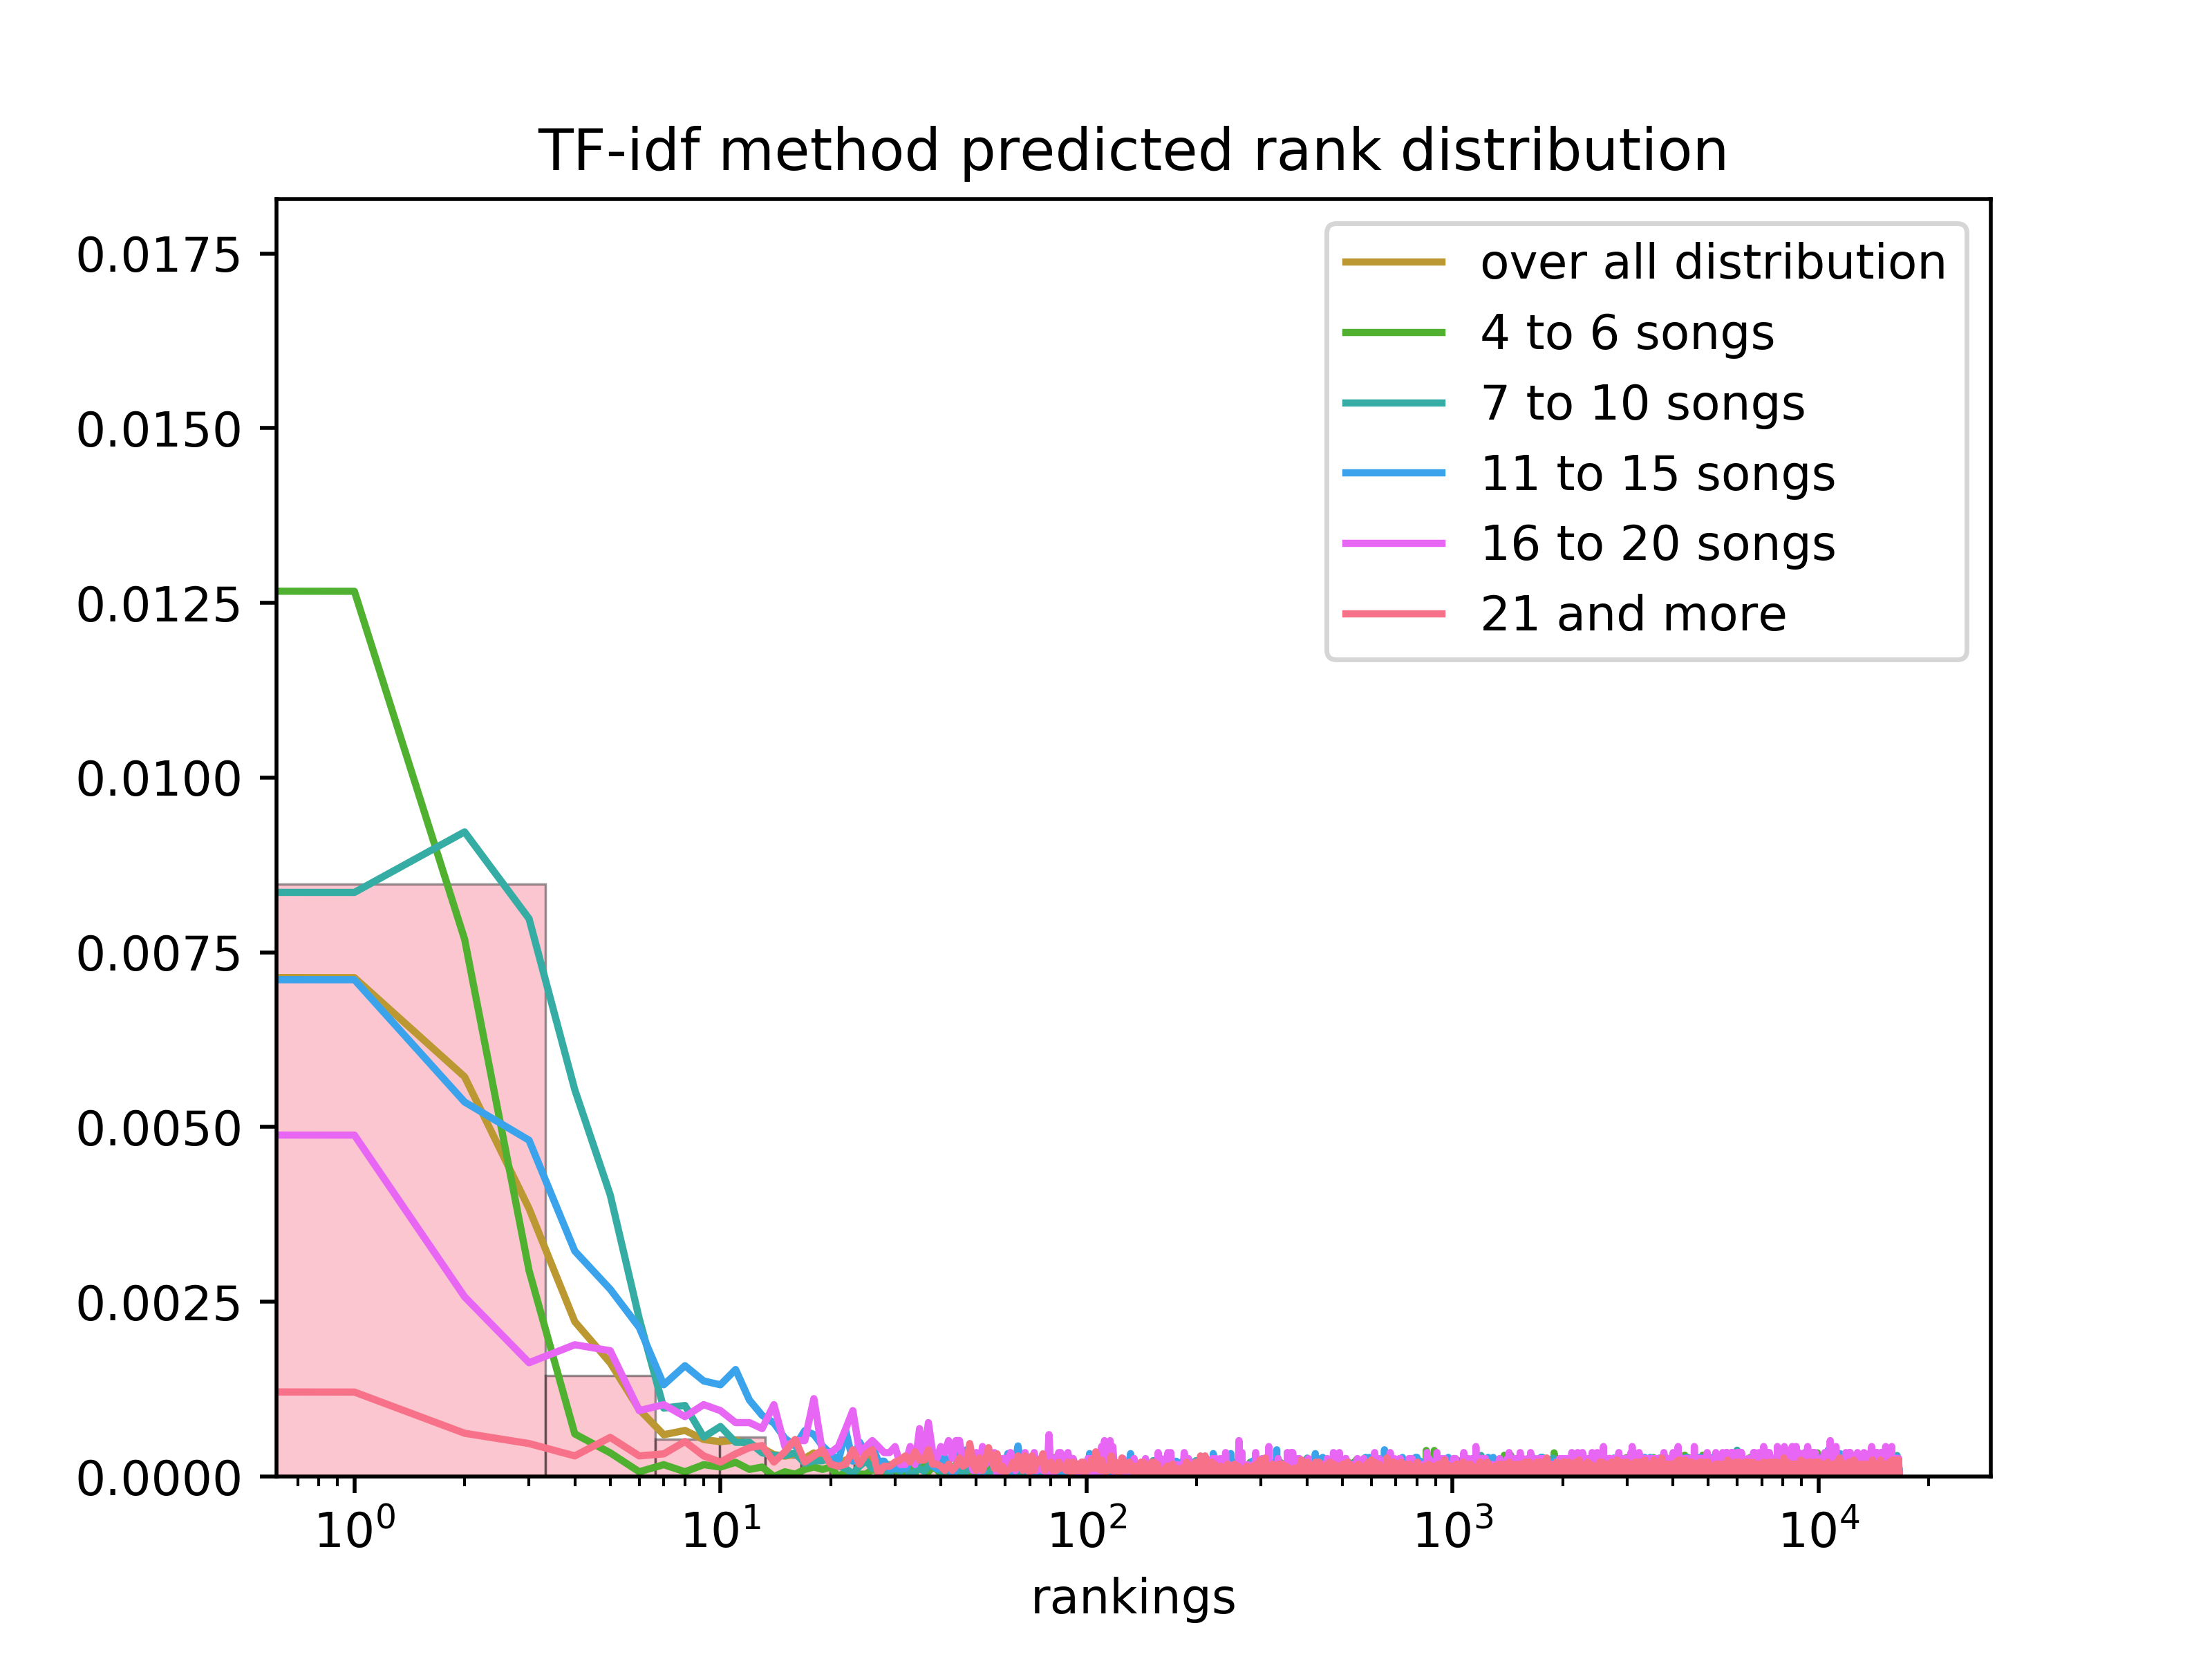
\includegraphics[width=1\linewidth]{./img/tf_idf_graph.png}
  \caption{RDG of the TF-idf method}
  \label{fig:tf_idf_distribution}
\end{minipage}%
 \vspace{1cm}
\begin{minipage}{.45\textwidth}
  \centering
  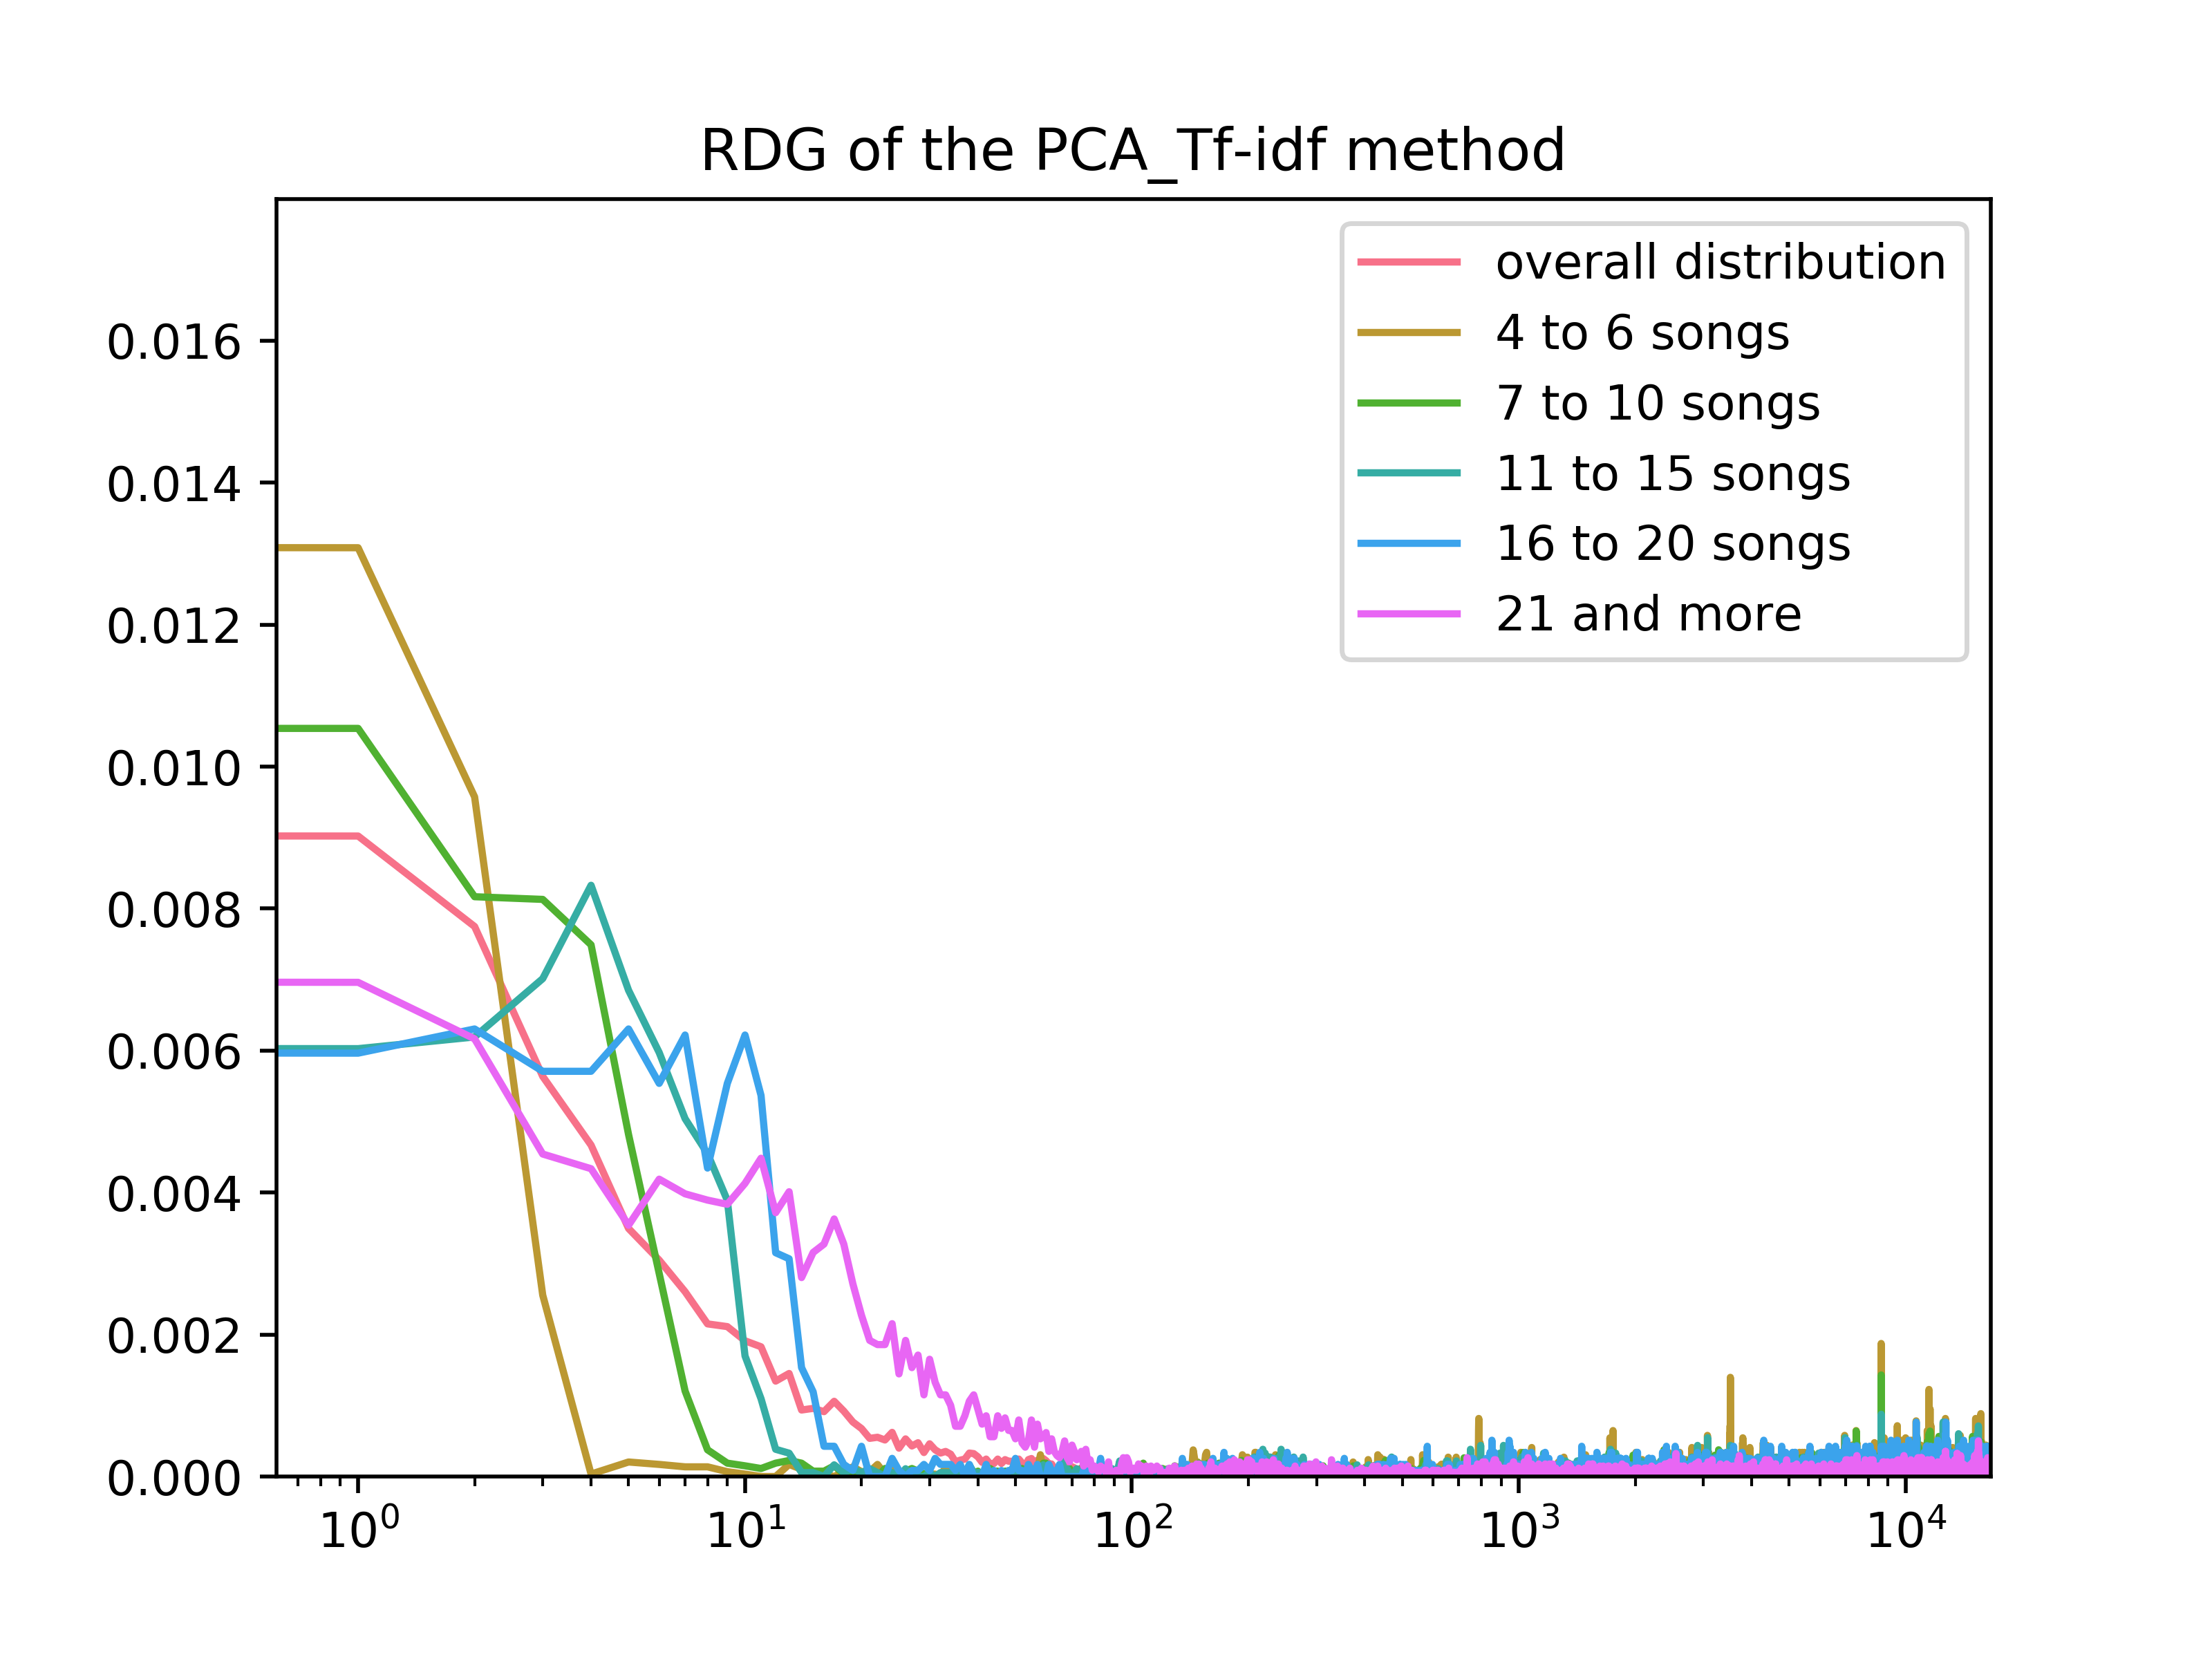
\includegraphics[width=1\linewidth]{./img/pca_tf_idf_graph.png}
  \caption{RDG of the PCA\_Tf-idf method}
  \label{fig:pca_tf_idf_distribution}
\end{minipage}
\end{figure}

\subsection{PCA\_Tf-idf results}\label{ssec:pca_tf-idf_results}

The results of the PCA-reduced Tf-idf vectors turned out to be better then full Tf-idf vectors. As we can see in Table \ref{table:1} the numbers are better for the \textit{R10} and \textit{R50}. The \textit{R@100} the values are almost the same. Figure \ref{fig:threshold_method_comparison} illustrates the fact, that after the application of the threshold, this method became the best one for long playlists and also the best method overall overtaking the PCA\_mel\_5715 which was the best method when defining similarity without threshold as can be seen in Figure \ref{fig:no_threshold_method_comparison}. 

\subsection{W2V results}\label{ssec:w2v_results}

\subsubsection{Results}
The small size of the vectors being produced by the W2V method are a significant advantage of this method. However the evaluation-measure values it yielded make it average to below average compared to methods. In ought to be mentioned that methods producing vectors of similar length such as PCA\_mel\_320 outperform the W2V.

\begin{table}[h]
\centering
\renewcommand{\arraystretch}{1.5}
\begin{tabu} to 1\textwidth { | c || X[c] | X[c] | X[c] | X[c] | X[c] |}
 \hline
 \textbf{method} & \textbf{R@10} & \textbf{R@50} & \textbf{R@100} & \textbf{nGDC} & $ \boldsymbol{\overline{rank}} $ \\
 \hline
 \hline
 W2V & 0.03519 & 0.04780 & 0.05544 & 0.030313 & 7804 \\
 \hline
\end{tabu} \\
\caption{Table summarizing average W2V evaluation values averaged over the 5 cross validation that were performed}
\label{table:2}
\end{table}

Table \ref{table:2} shows lower numbers than for the Tf-idf method. 3.5\% of songs from the $ p_{test} $ set ranked in the top 10, 4.8\% in top 50 and 5.5\% in top 100. The average rank was 7804. When looking at the distribution graph, it is very clear that the gap between the number of predicted ranks within the first 5 ranks for short and longer playlists is big and Figures \ref{fig:no_threshold_method_comparison} and \ref{fig:threshold_method_comparison} show us, that the threshold helped this method especially for ranking of songs from longer playlists, where it even outmatched the PCA\_mel\_320. 

\begin{figure}[h]
    \centering
	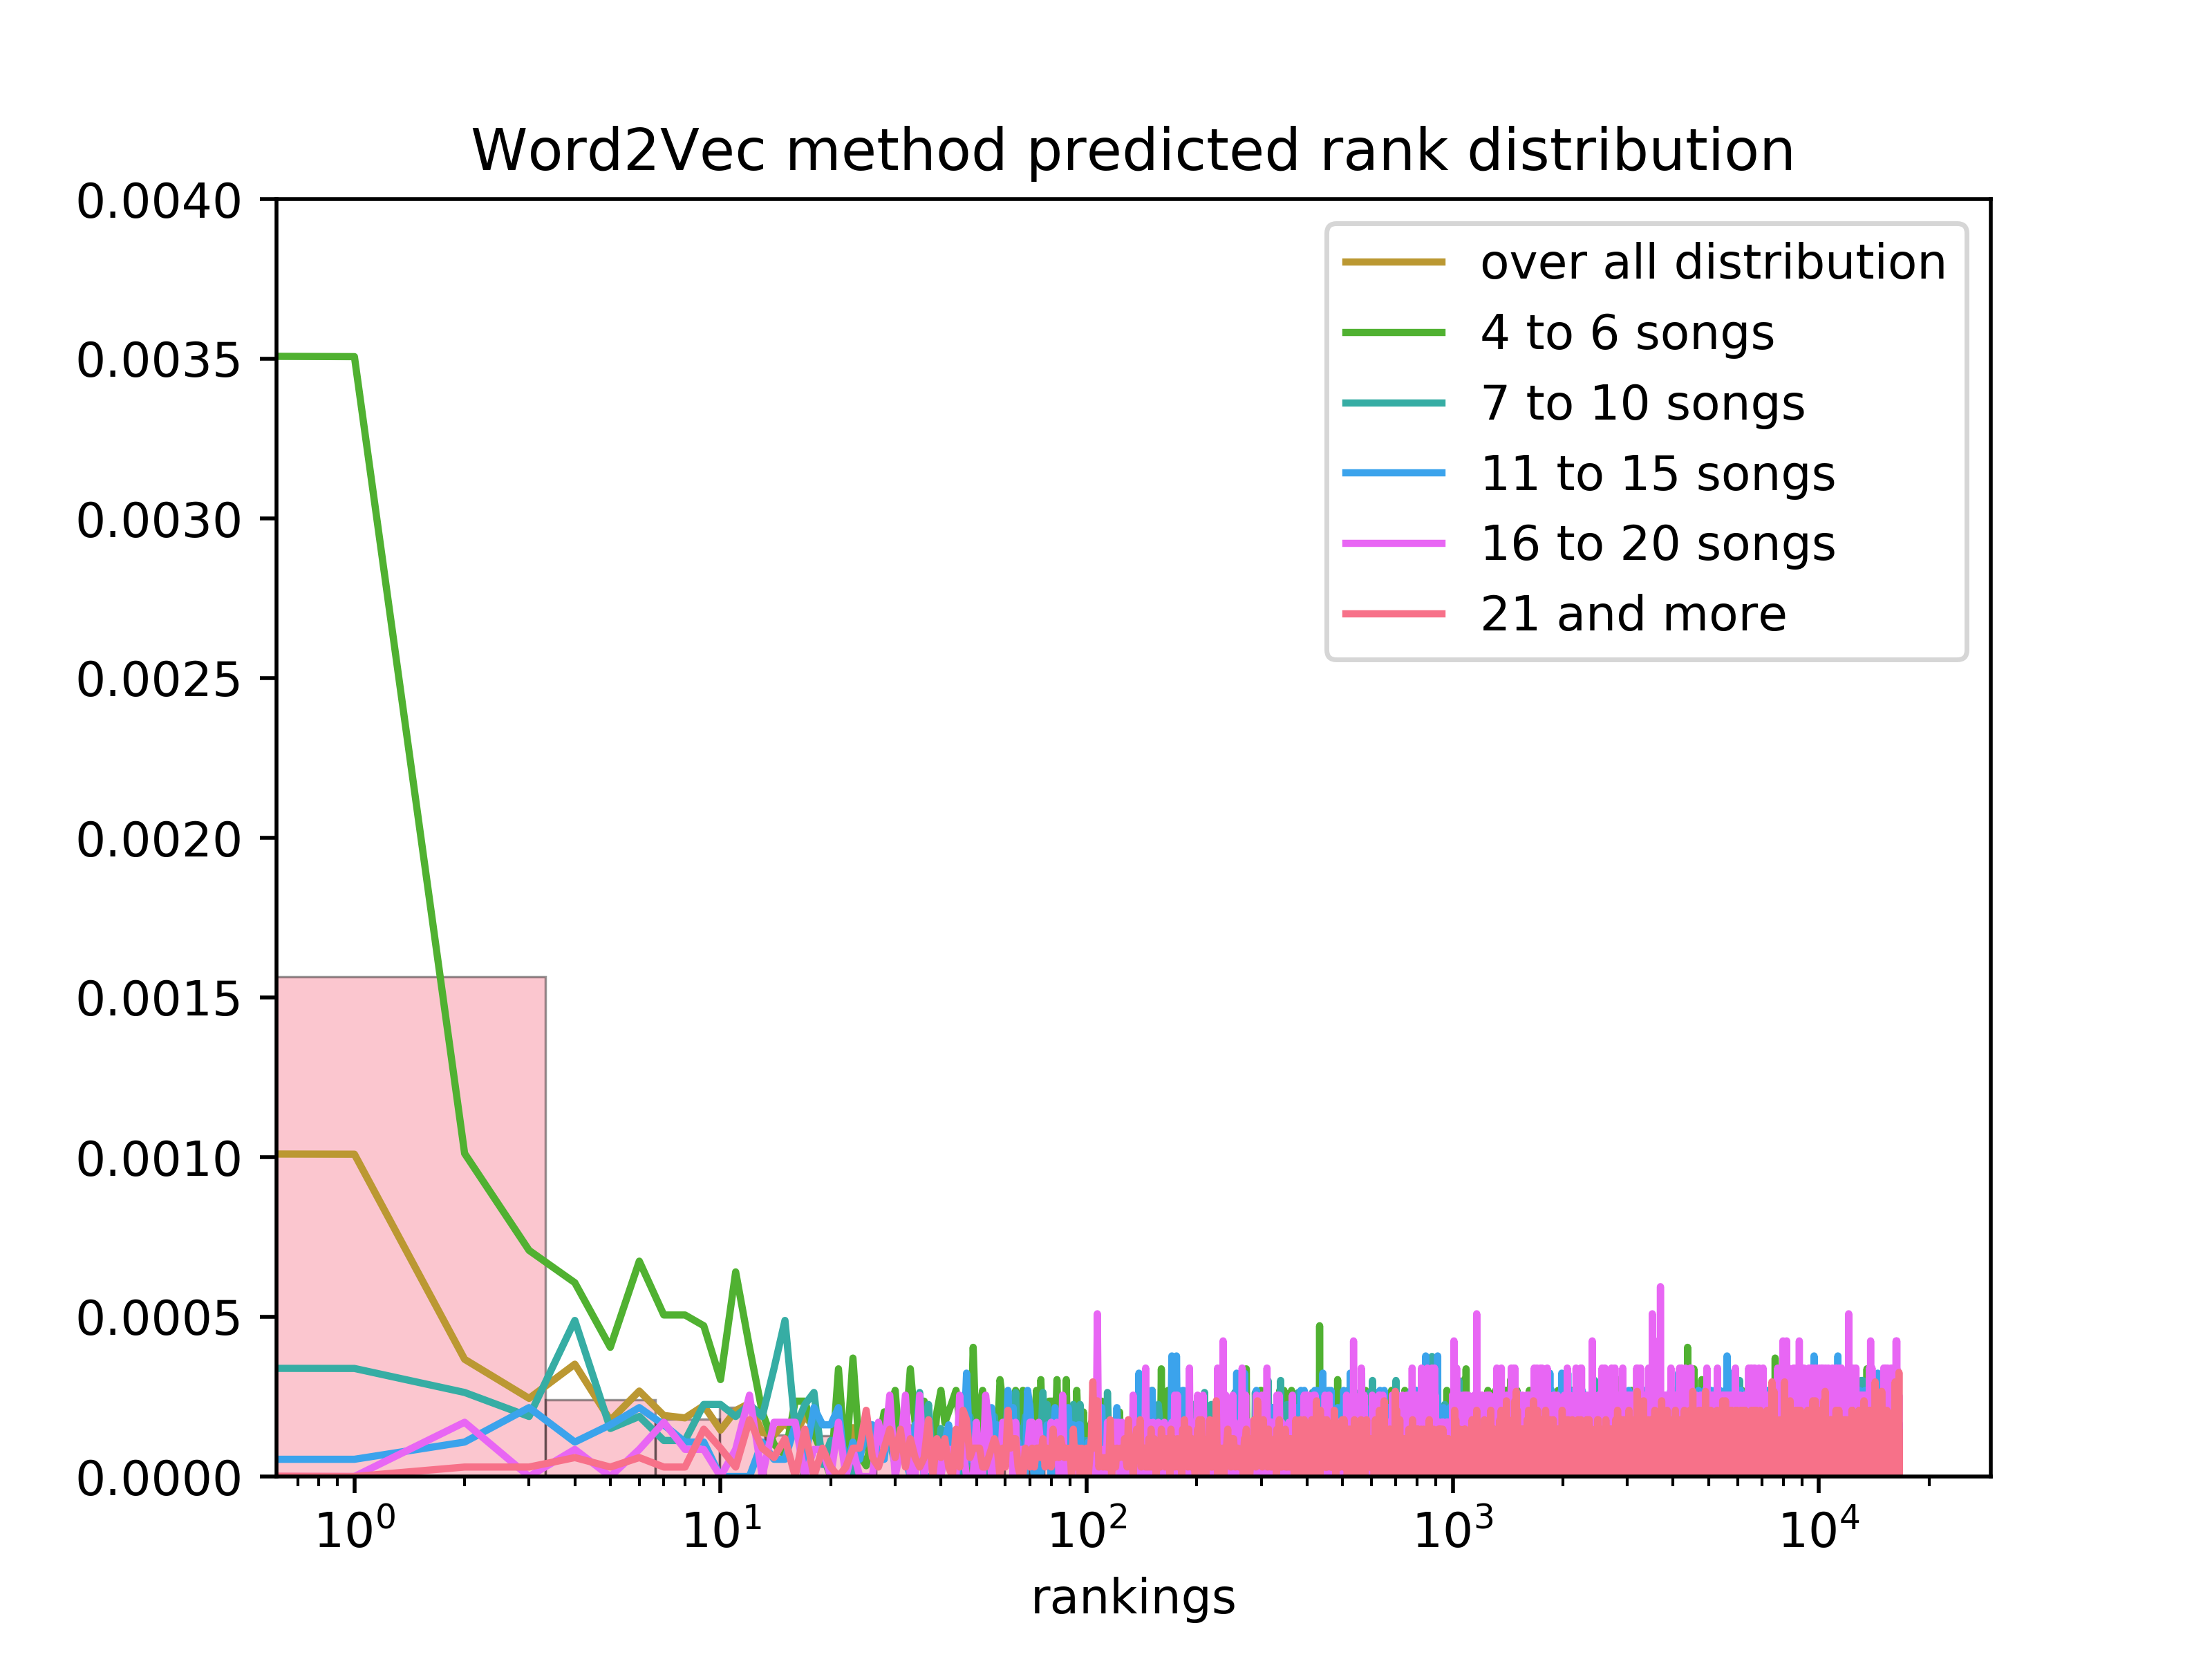
\includegraphics[width=120mm]{./img/w2v_graph.png}
	\caption{Distribution of ranks of songs from the test set the w2v method assigned them.}
	\label{fig:w2v_distribution}
\end{figure}

\subsection{SOM results}\label{ssec:som_results}

\begin{figure}
    \centering
	\includegraphics[width=140mm]{./img/som_map.png}
	\caption{The location of different songs from 20 randomly selected playlists on the map created by SOM. Each playlist has its own colour.}
	\label{fig:som_map}
\end{figure}

\subsubsection{Results}
When we then tried to display resulting SOM map with all the songs, the size of the image would have to be immense for all 16,594 songs to be recognizable. The problem was that there are many songs to display on the map and the titles and artists overlap. Because of that, we decided to randomly select 20 playlists and show where the different songs that belong to each playlist are placed on the map. Each playlist has its own color. The playlist map for the SOM with W2V input is depicted in Figure \ref{fig:som_map}. The playlists do not really form any visible clusters which suggests that songs that should be similar because they are in the same playlist are not close to each other in the space created by the SOM\_W2V. 

This observation supports the results for the self organizing map algorithm which are quite poor. Actually, it is the worse method that we implemented and our hope to enhance the results of W2V were not fulfilled. The threshold did not make it better either. The results improved but it still stayed at the bottom of the method rankings as the dark red color in Figure \ref{fig:threshold_method_comparison} suggests.

\begin{table}[h]
\centering
\renewcommand{\arraystretch}{1.5}
\begin{tabu} to 1\textwidth { | c || X[c] | X[c] | X[c] | X[c] | X[c] |}
 \hline
 \textbf{method} & \textbf{R@10} & \textbf{R@50} & \textbf{R@100} & \textbf{nGDC} & $ \boldsymbol{\overline{rank}} $ \\
 \hline
 \hline
 SOM with W2V & 0.00103 & 0.00427 & 0.00720 & 0.00200 & 8034 \\
 \hline
 SOM wiht PCA\_Tf-idf & 0.00044 & 0.00208 & 0.00462 & 0.00125 & 8243 \\
 \hline
\end{tabu} \\
\caption{Table summarizing average SOM evaluation values averaged over the 5 cross validations}
\label{table:som}
\end{table}

The RDG of the SOM\_W2V method clearly shows, that the distribution of ranks is random or worse. The main reason for the failure of this method is unclear but it is possible that the data from the W2V vectors compress the information so much, that the SOM network is not able to cluster data based on it. But since we received even worse results for the SOM\_Tf-id as can be seen in Figure \ref{fig:som_tf_idf_distribution} and Table \ref{table:som} we are more inclined to another possibility which is, that the SOM network is not able to provide satisfying results because two dimensions are simply too little to represent input data of such complexity.

\begin{figure}[H]
\centering
\begin{minipage}{.45\textwidth}
  \centering
  	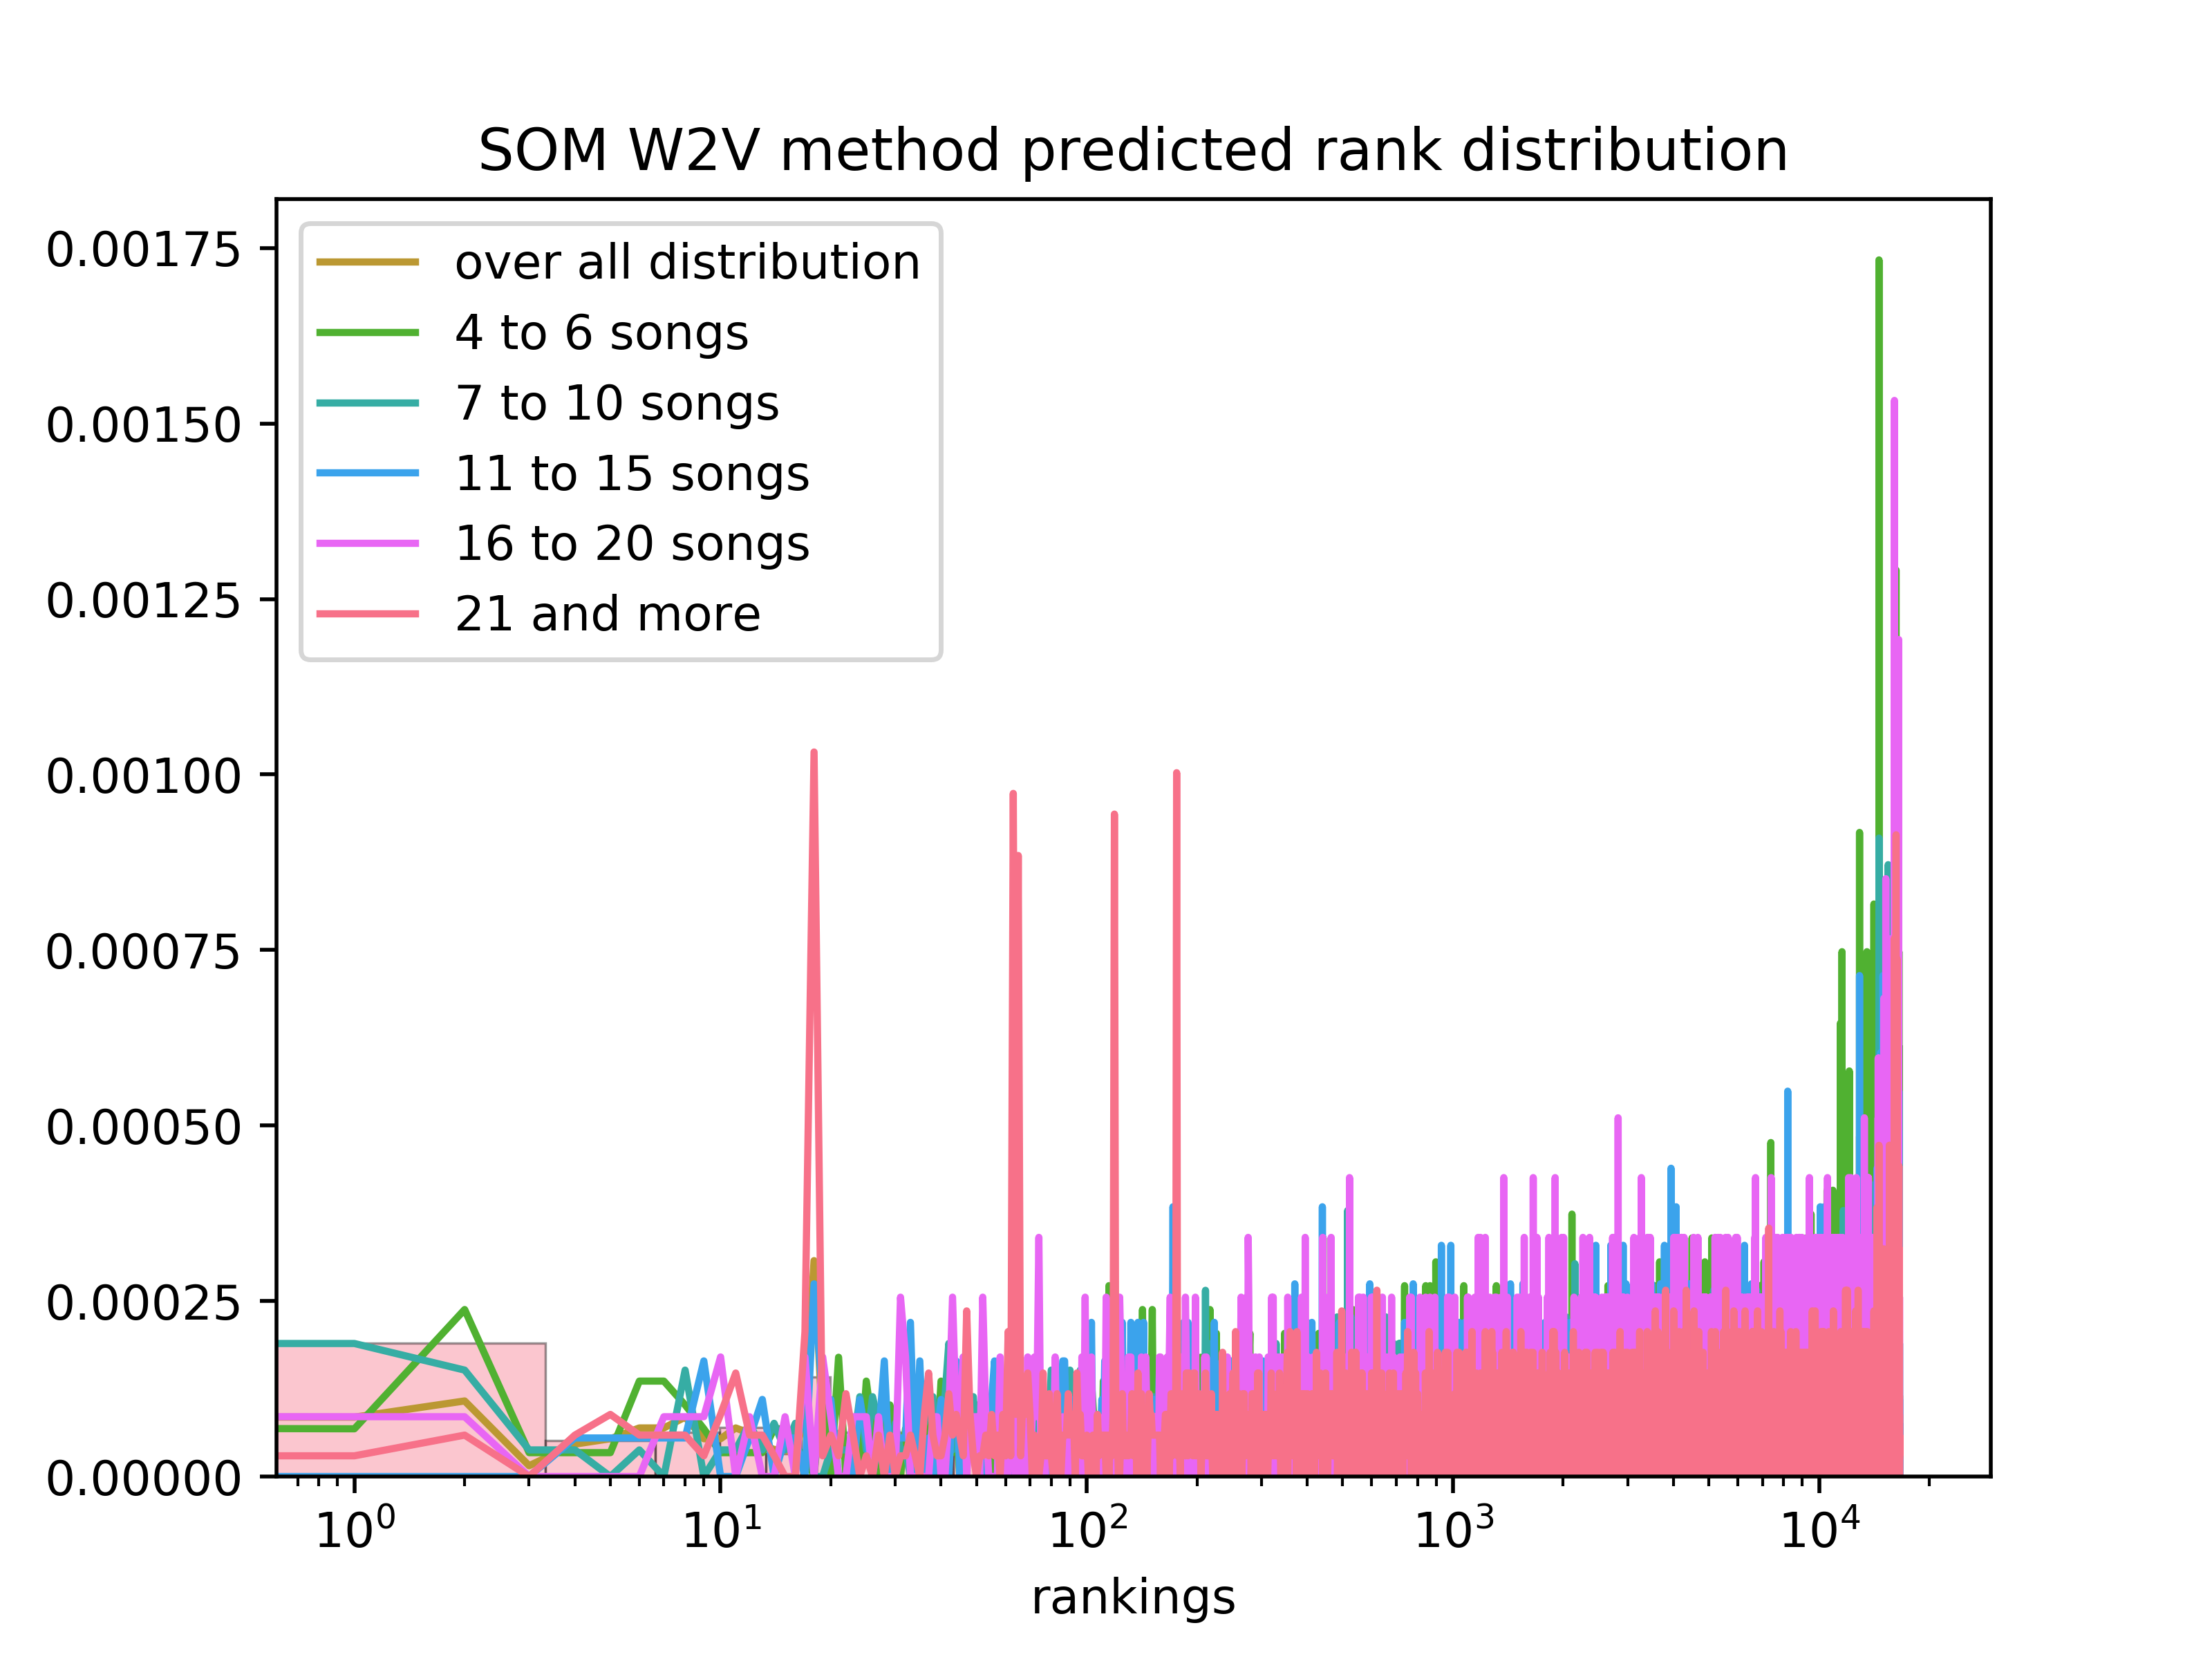
\includegraphics[width=1\linewidth]{./img/som_w2v_graph.png}
	\caption{RDG of the SOM\_W2V method}
	\label{fig:som_distribution}
\end{minipage}%
 \vspace{1cm}
\begin{minipage}{.45\textwidth}
  \centering
  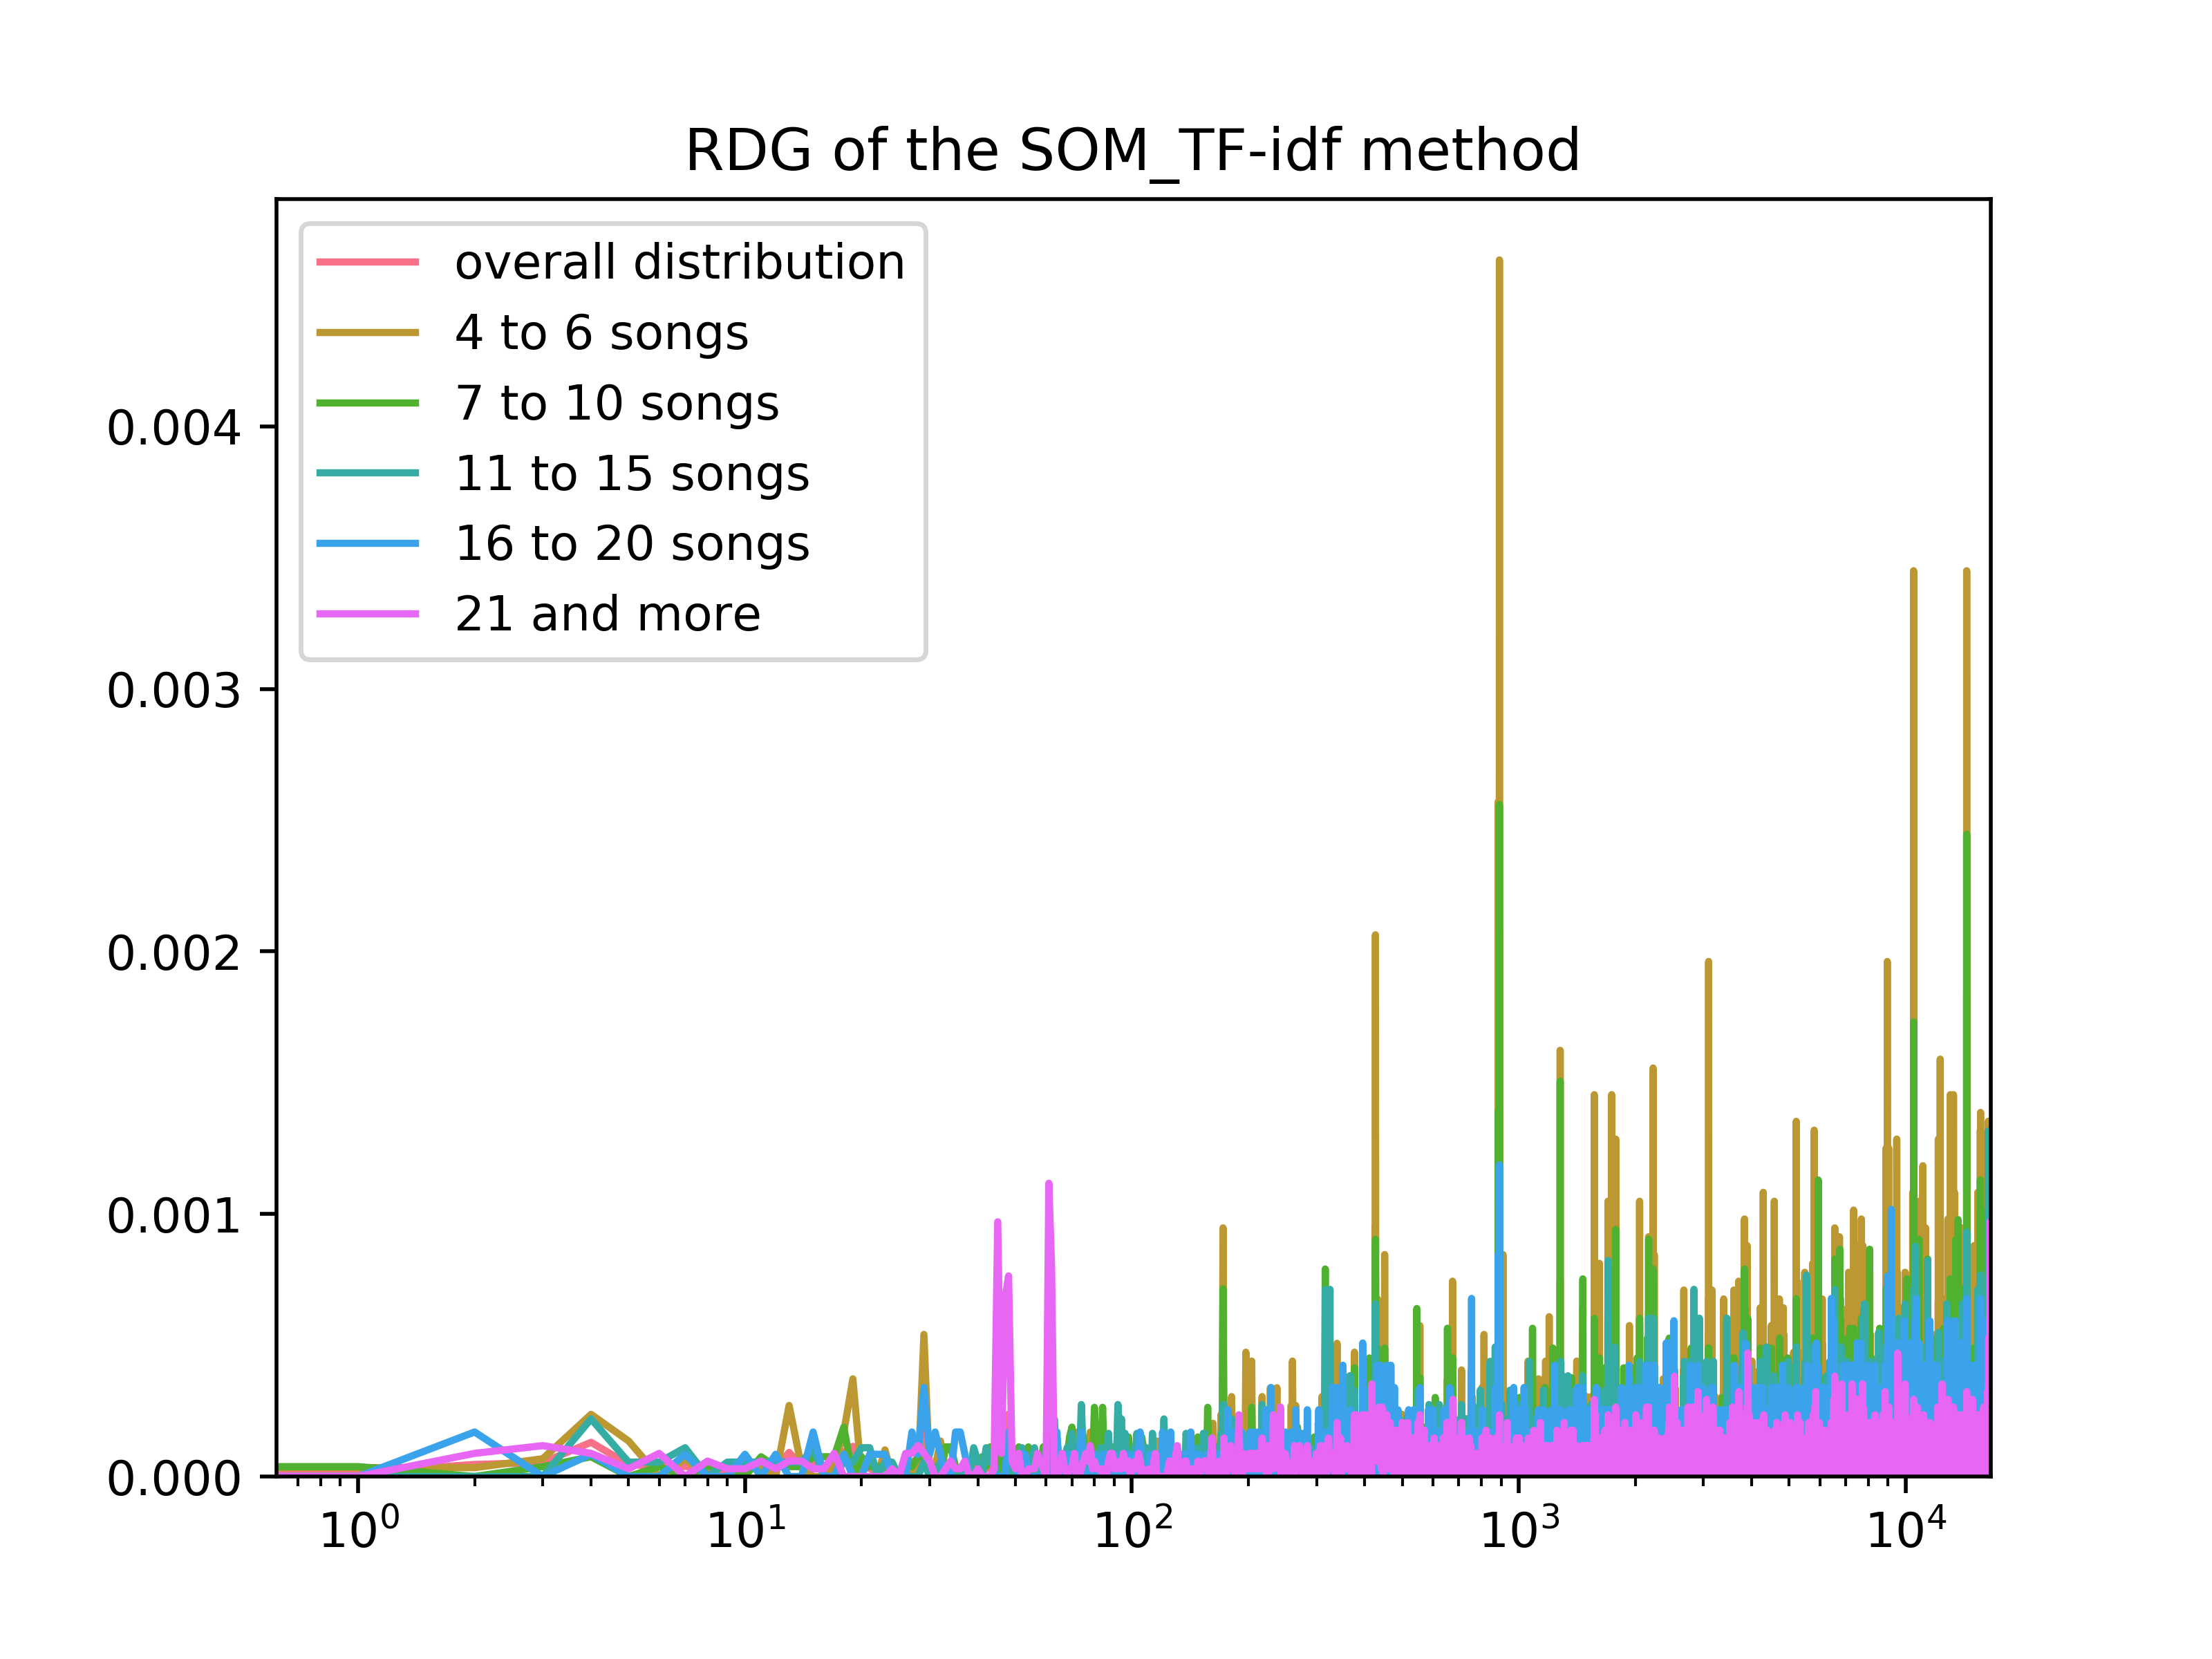
\includegraphics[width=1\linewidth]{./img/som_tf_idf_graph.png}
  \caption{RDG of the SOM\_Tf-idf method}
  \label{fig:som_tf_idf_distribution}
\end{minipage}
\end{figure}

\section{Simple audio representation results}\label{sec:simple_audio_resutls}
\subsection{Raw mel-spectrogram results}\label{ssec:mel_results}

As can be seen in Table \ref{table:mel_spec_methods} with raw mel-spectrograms, 3.7\% of songs ended up between top ten predictions, 4.3\% between the top 50 and 4.7\% in between the top 100. These results are actually better than any other method using mel-spectrograms as input was before applying the threshold, except of the two PCA\_mel methods.

\subsubsection{Results}
\begin{table}[H]
\centering
\renewcommand{\arraystretch}{1.5}
\begin{tabu} to 1\textwidth { | c || c | c | c | c | c |}
 \hline
 \textbf{method} & \textbf{R@10} & \textbf{R@50} & \textbf{R@100} & \textbf{nGDC} & $ \boldsymbol{\overline{rank}} $ \\
 \hline
 \hline
 Raw mel-spectrograms & 0.03696 & 0.04275 & 0.0473 & 0.03063 & 7604 \\
 \hline
 PCA\_mel\_5715 & 0.05287 & 0.06298 & 0.06765 & 0.04317 & 7803 \\
 \hline
 PCA\_mel\_320 & 0.04716 & 0.05928 & 0.06550 & 0.03989 & 8357 \\
 \hline
 GRU\_mel  & 0.04628 & 0.05715 & 0.06285 & 0.03856 & 7601 \\
 \hline
 LSTM\_mel & 0.03197 & 0.04291 & 0.04978 & 0.02750 & 7776\\
 \hline
\end{tabu} \\
\caption{Table summarizing average evaluation values for all methods with mel-spectrogram input averaged over 5 cross validations with threshold.}
\label{table:mel_spec_methods}
\end{table}
The patterns observed in Figure \ref{fig:raw_mel_graph} display the same tendencies as all other methods we are studying (except of those that appear to be random such as SOM). The short playlists go through a sharp drop at the beginning. Longer playlists are worse in the beginning as the top ranks for them are a bit less numerous, especially for playlists of length 21 and more but they drop more steadily. 

\begin{figure}[H]
    \centering
	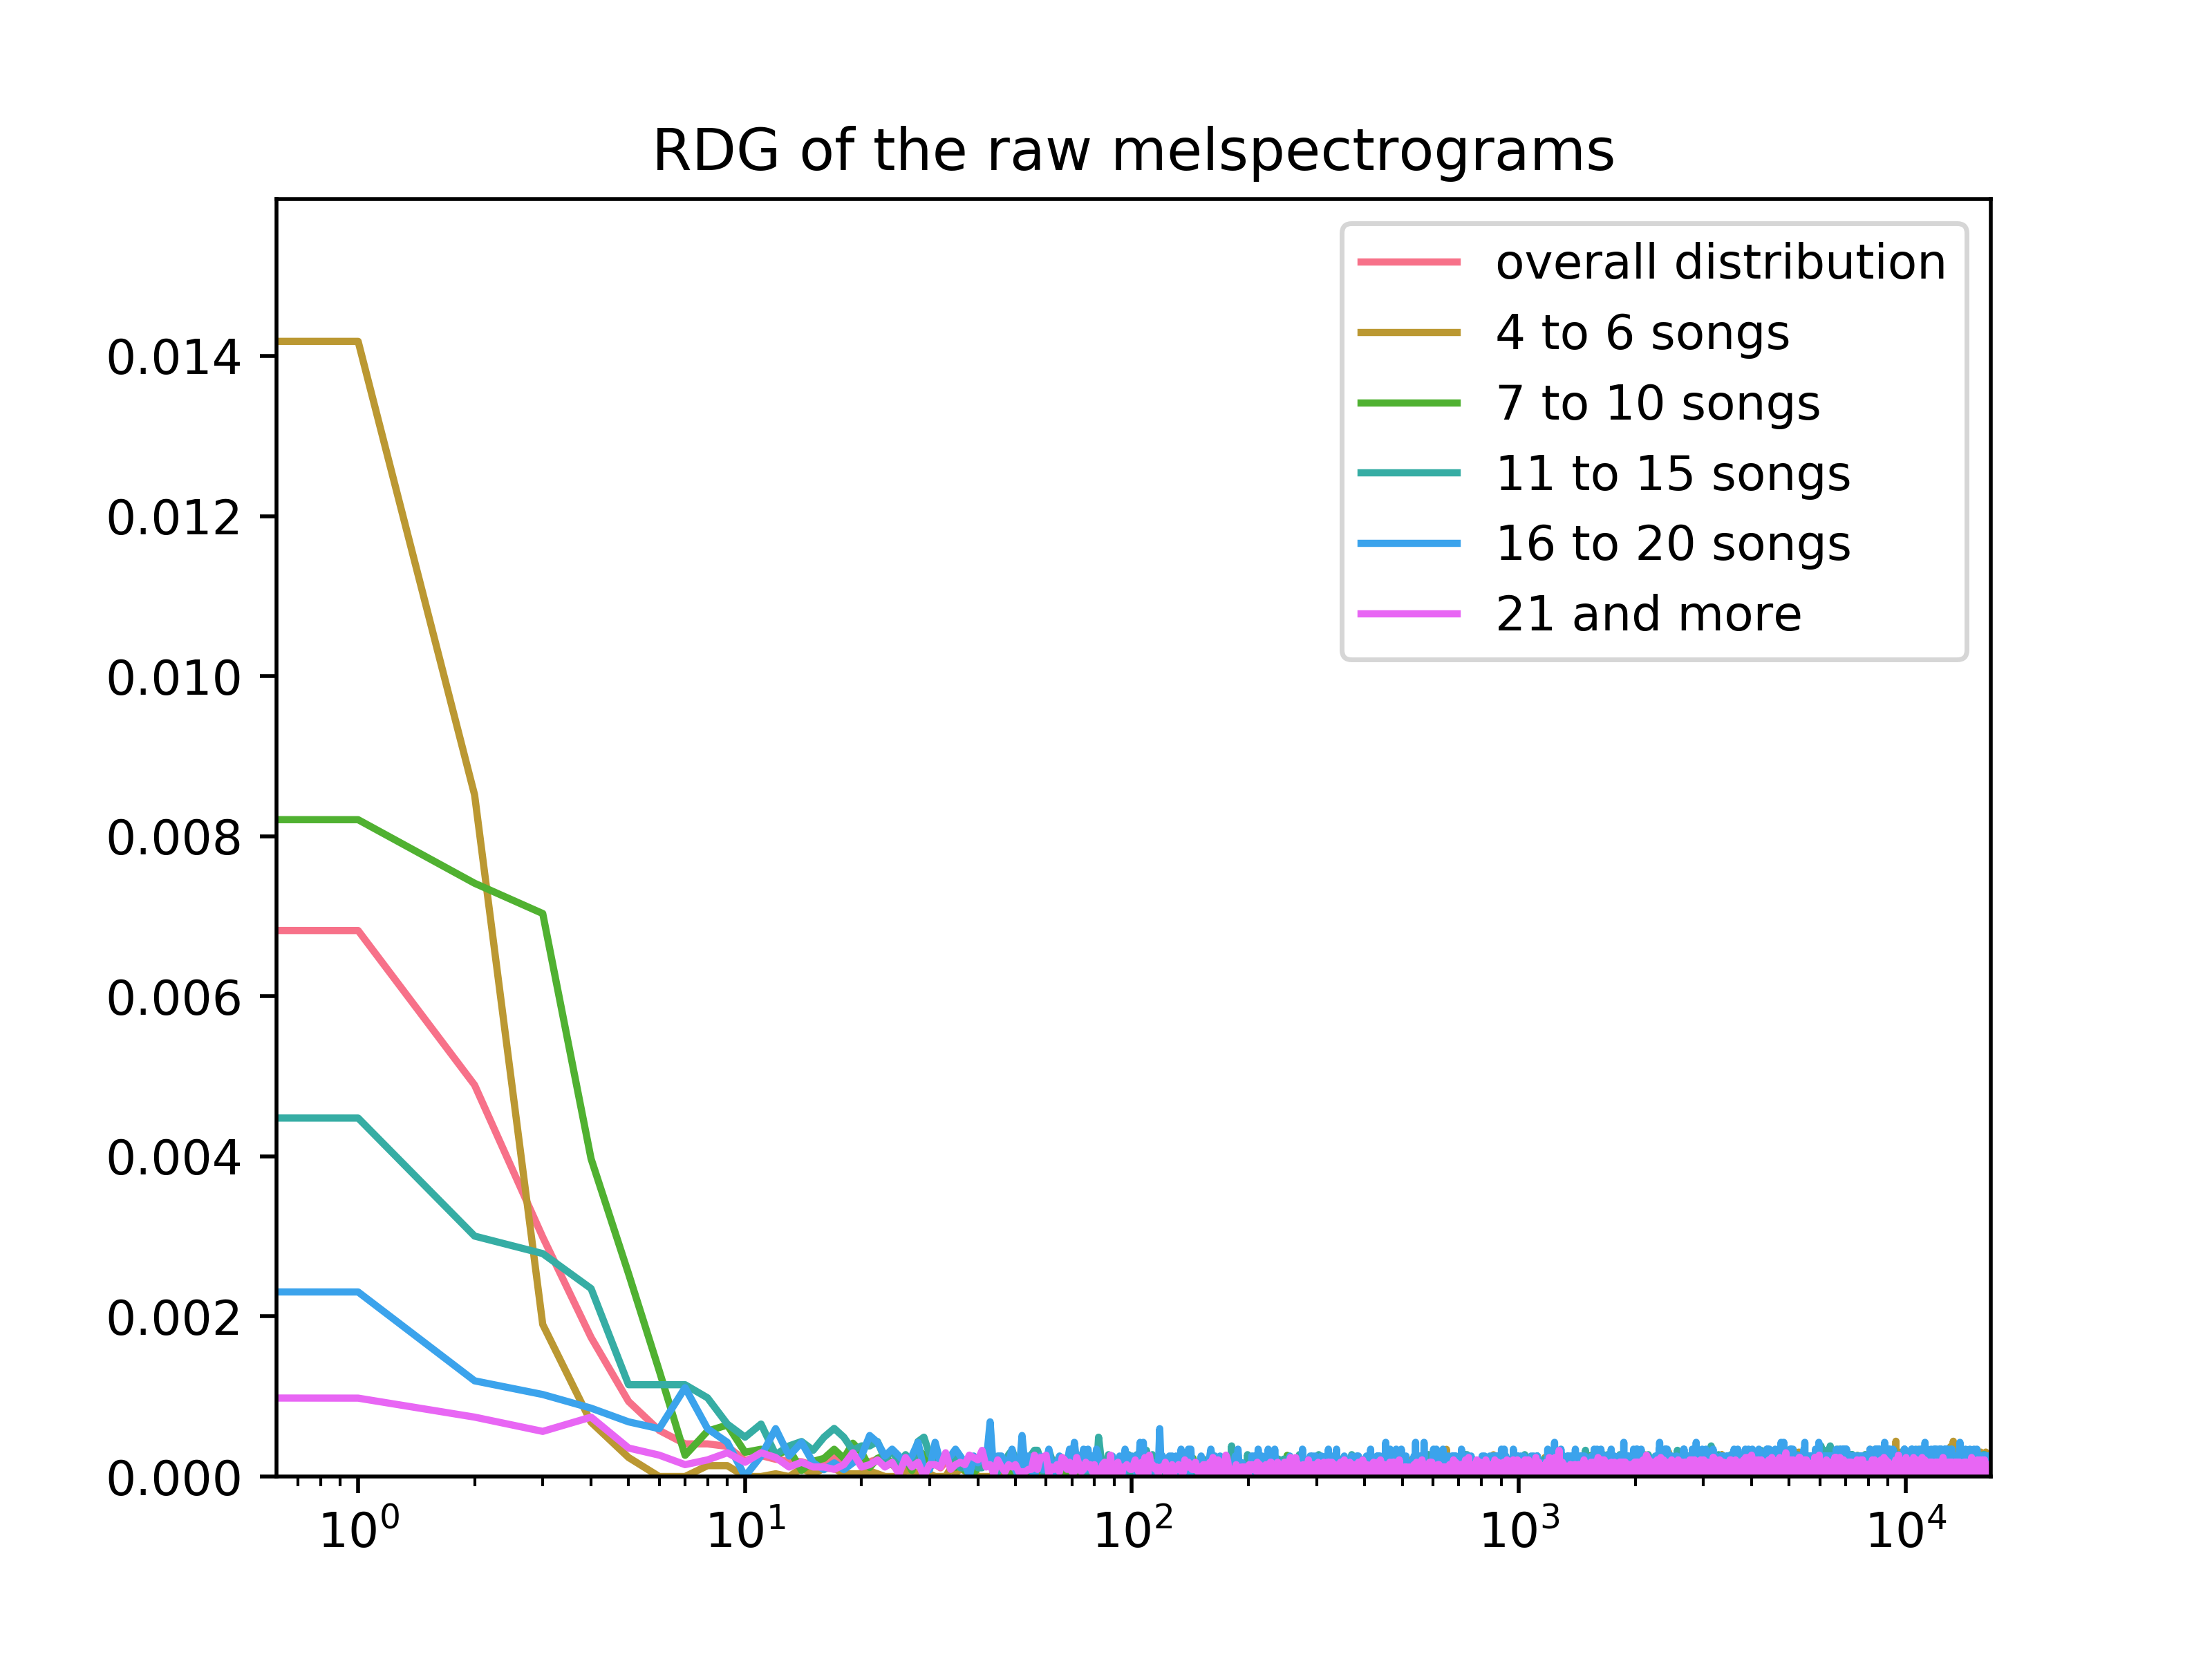
\includegraphics[width=120mm]{./img/raw_mel_graph.png}
	\caption{RDG of raw Mel-spectrograms.}
	\label{fig:raw_mel_graph}
\end{figure}

\subsection{Raw MFCCs results}\label{ssec:raw_mfccs_results}

The results of raw MFCCs are quite poor compared to other methods. Only 0.4\% of songs rank between the top 10, 0.9\% in the top 50 and 1.4\% in the top 100 as we can see in Table \ref{table:mfcc_methods}. It was better than the LSTM\_MFCC method before we applied the threshold to our evaluation but not very good overall.
\begin{table}[H]
\centering
\renewcommand{\arraystretch}{1.5}
\begin{tabu} to 1\textwidth { | c || X[c] | X[c] | c | X[c] | X[c] |}
 \hline
 \textbf{method} & \textbf{R@10} & \textbf{R@50} & \textbf{R@100} & \textbf{nGDC} & $ \boldsymbol{\overline{rank}} $ \\
 \hline
 \hline
 Raw MFCC & 0.00415 & 0.00919 & 0.01423 & 0.00607 &  7552 \\
 \hline
 LSTM\_MFCC & 0.03887 & 0.04935 & 0.05670 & 0.033058 & 7774 \\
 \hline
 GRU\_MFCC & 0.03769 & 0.04737 & 0.05438 & 0.032151 & 7774 \\
 \hline
\end{tabu} \\

\caption{Table summarizing average evaluation values for all methods with MFCC input averaged over 5 cross validations with threshold.}
\label{table:mfcc_methods}
\end{table}

 When looking at the traditional RDG, we again observe a drop for short playlists, not as sharp as for other methods though. Nevertheless, the rankings for longer playlists, do not seem to be very stable and this method does not behave as a good recommendation method should.
 
\begin{figure}[H]
    \centering
	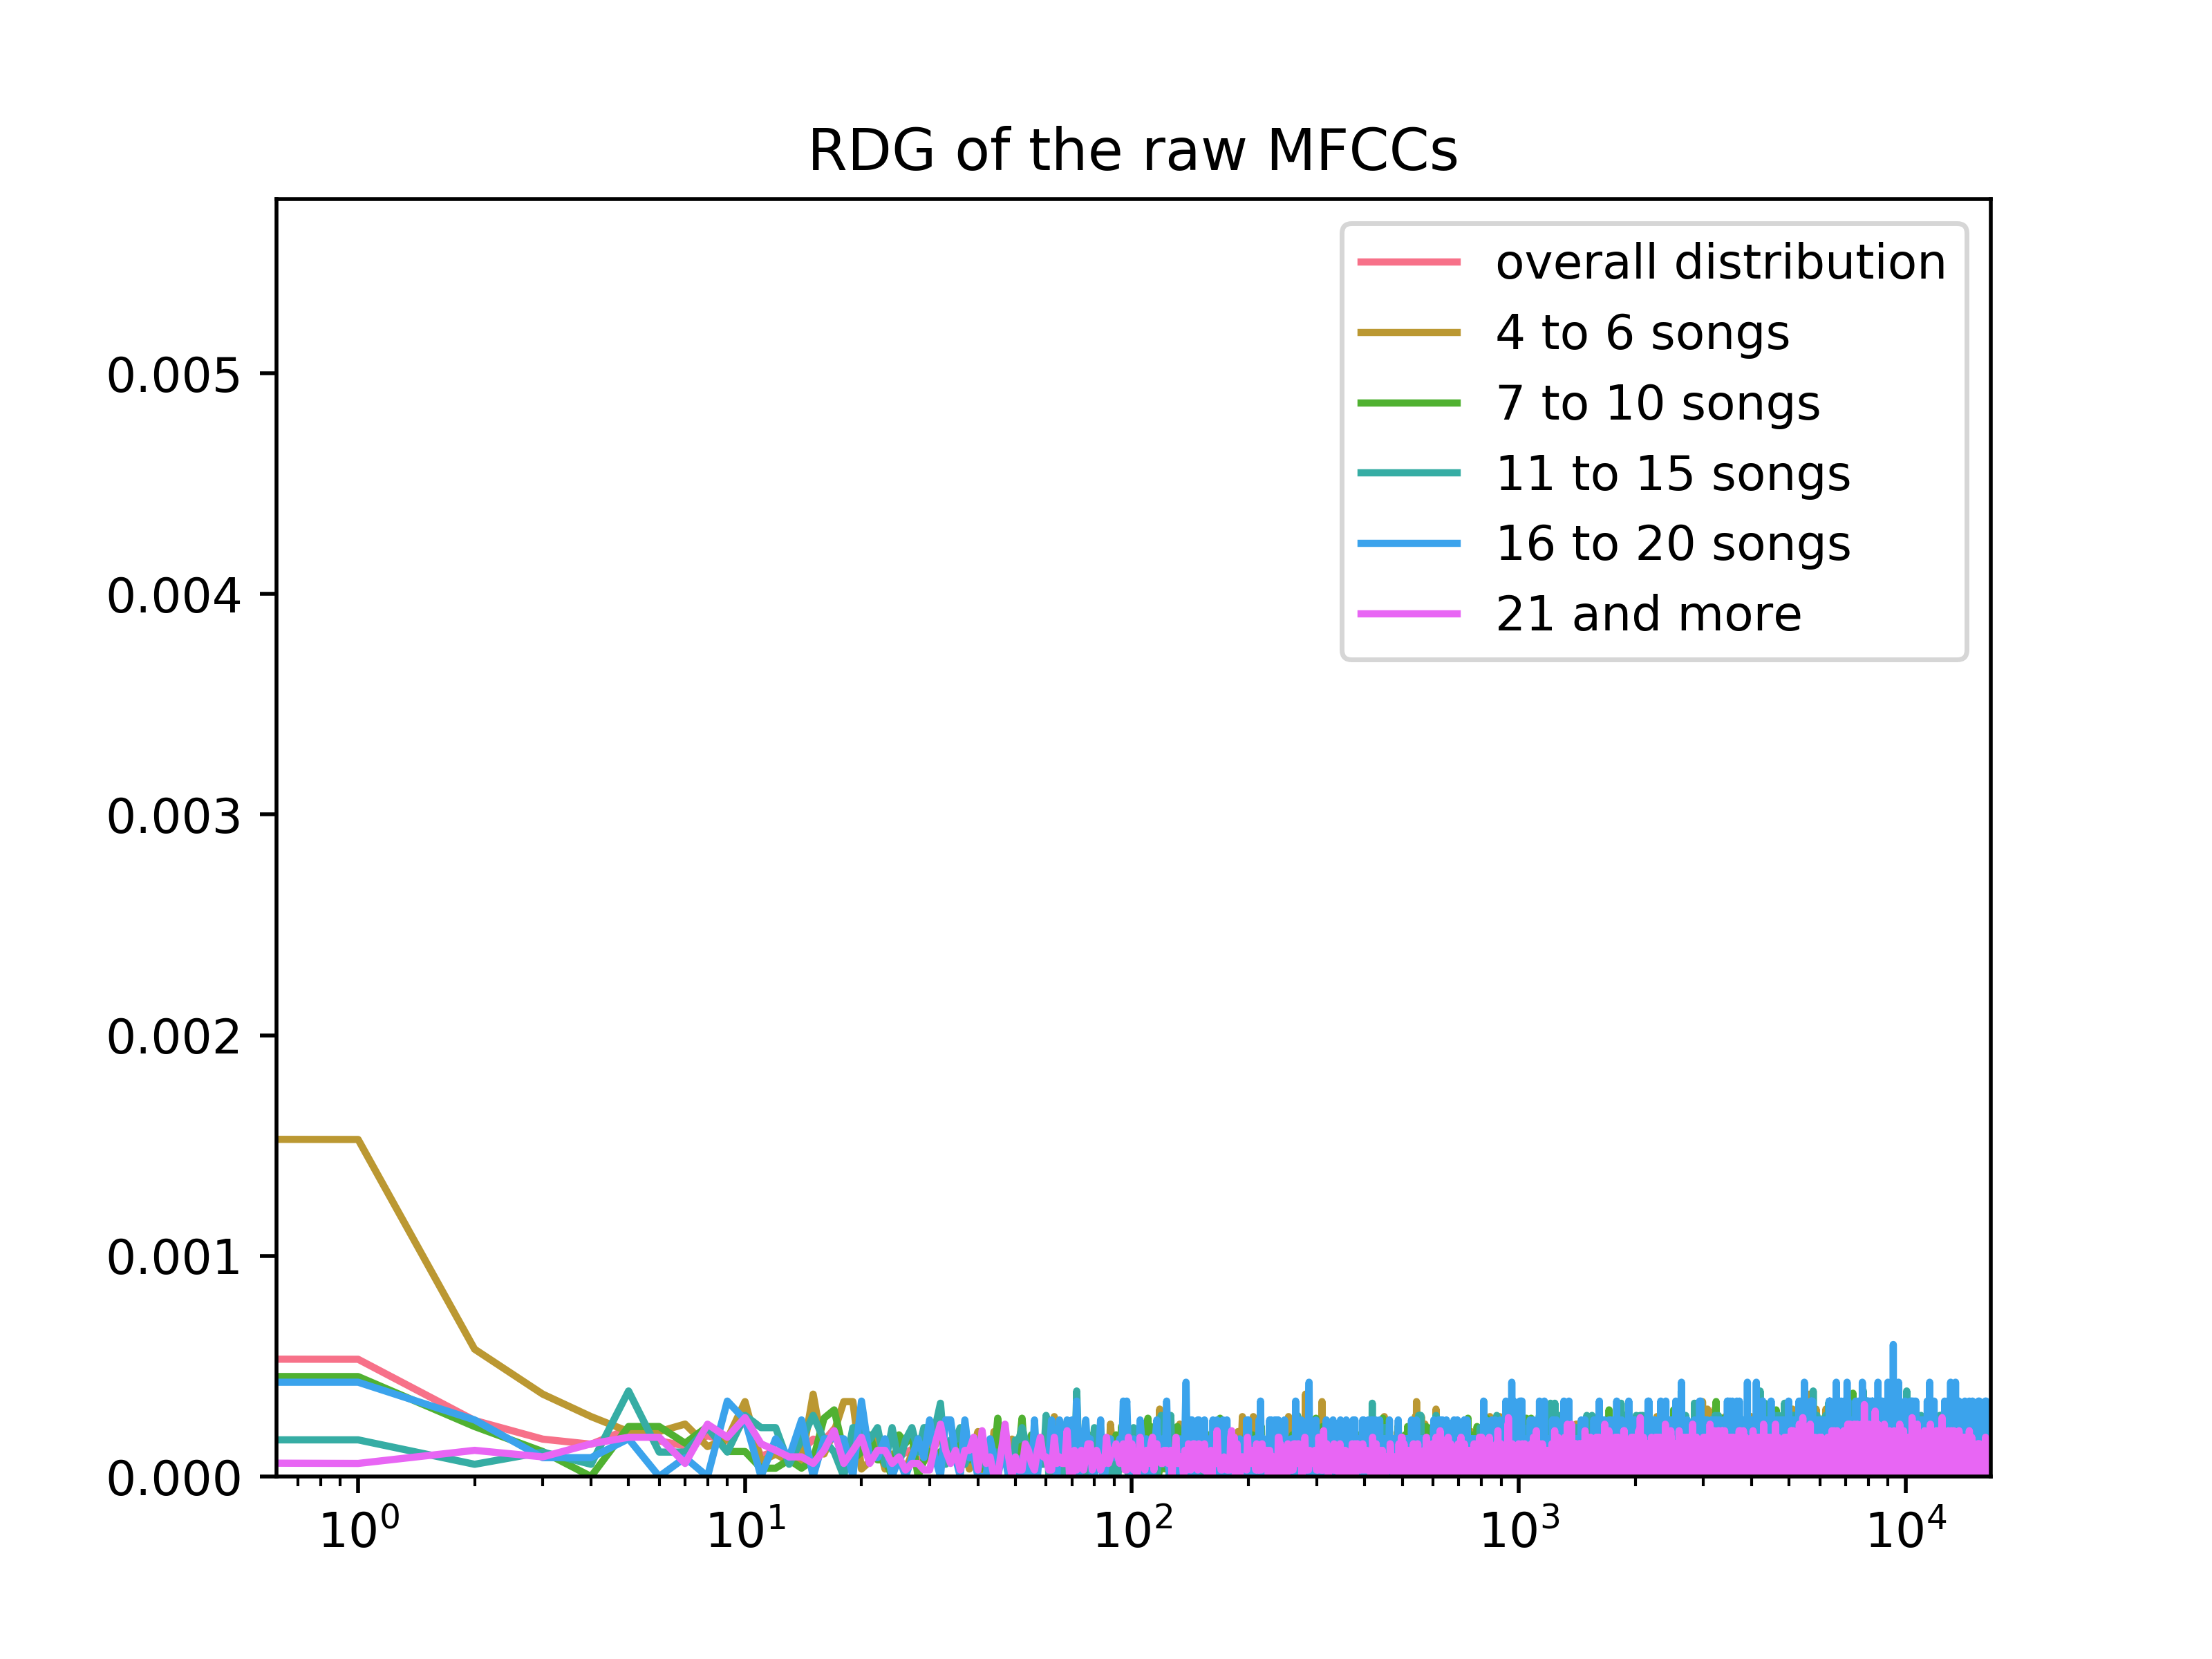
\includegraphics[width=120mm]{./img/mfcc_graph.png}
	\caption{RDG of raw MFCCs.}
	\label{fig:mfcc_graph}
\end{figure}

\subsection{PCA on spectrograms}\label{ssec:pca_spec_results}



The dimensionality reduction in this method was the biggest of all methods. Our song representation went from 900,048 to 1,106 respectively 320 dimensions.
Even with only 57\% of explained variance for the PCA\_spec\_1106, this method's results were above average compared to other methods. So it seemed reasonable to go for an even more radical reduction to vectors of length 320. The results of the method encoding songs into shorter vectors were only slightly worse than those of the one yielding longer vectors with similarity defined without threshold. 

One interesting thing is, that the PCA\_spec\_320 method is the only one whose results worsened with the application of the threshold and the gap between the performance of these two methods widened. It can be observed in Figure \ref{fig:no_threshold_method_comparison} where method ranking without the use of similarity with threshold is depicted and both methods are green, and Figure \ref{fig:threshold_method_comparison} where methods are ranked with using the threshold in the similarity definition and the PCA\_spec\_320 is in the orange area and the PCA\_spec\_1106 stays green.

\begin{table}[h]
\centering
\renewcommand{\arraystretch}{1.5}
\begin{tabu} to 1\textwidth { | c || c | c | c | c | c |}
 \hline
 \textbf{method} & \textbf{R@10} & \textbf{R@50} & \textbf{R@100} & \textbf{nGDC} & $ \boldsymbol{\overline{rank}} $ \\
 \hline
 \hline
 PCA\_spec\_1106 & 0.04747 & 0.05915 &  0.06472 & 0.03982 & 7797 \\
 \hline
 PCA\_spec\_320 & 0.03166 & 0.04289 &  0.05094 & 0.02890 & 7496 \\
 \hline
 GRU\_spec\_20400 & 0.04287 & 0.05196 & 0.05723 & 0.03563 & 7824 \\
 \hline
 GRU\_spec\_5712 & 0.00248 & 0.00628 & 0.01076 & 0.003757 & 7761 \\
 \hline
 LSTM\_spec\_20400 & 0.03641 & 0.05096 & 0.05921 & 0.03126 & 7786 \\
 \hline
 LSTM\_spec\_5712 & 0.01892 & 0.03263 & 0.04252 &  0.01899 & 7643 \\
 \hline
\end{tabu} \\
\caption{Table summarizing average evaluation values for methods with spectrogram input averaged over 5 cross validations}
\label{table:spec_methods}
\end{table}
 
\begin{figure}[h]
\centering
\begin{minipage}{.45\textwidth}
  \centering
  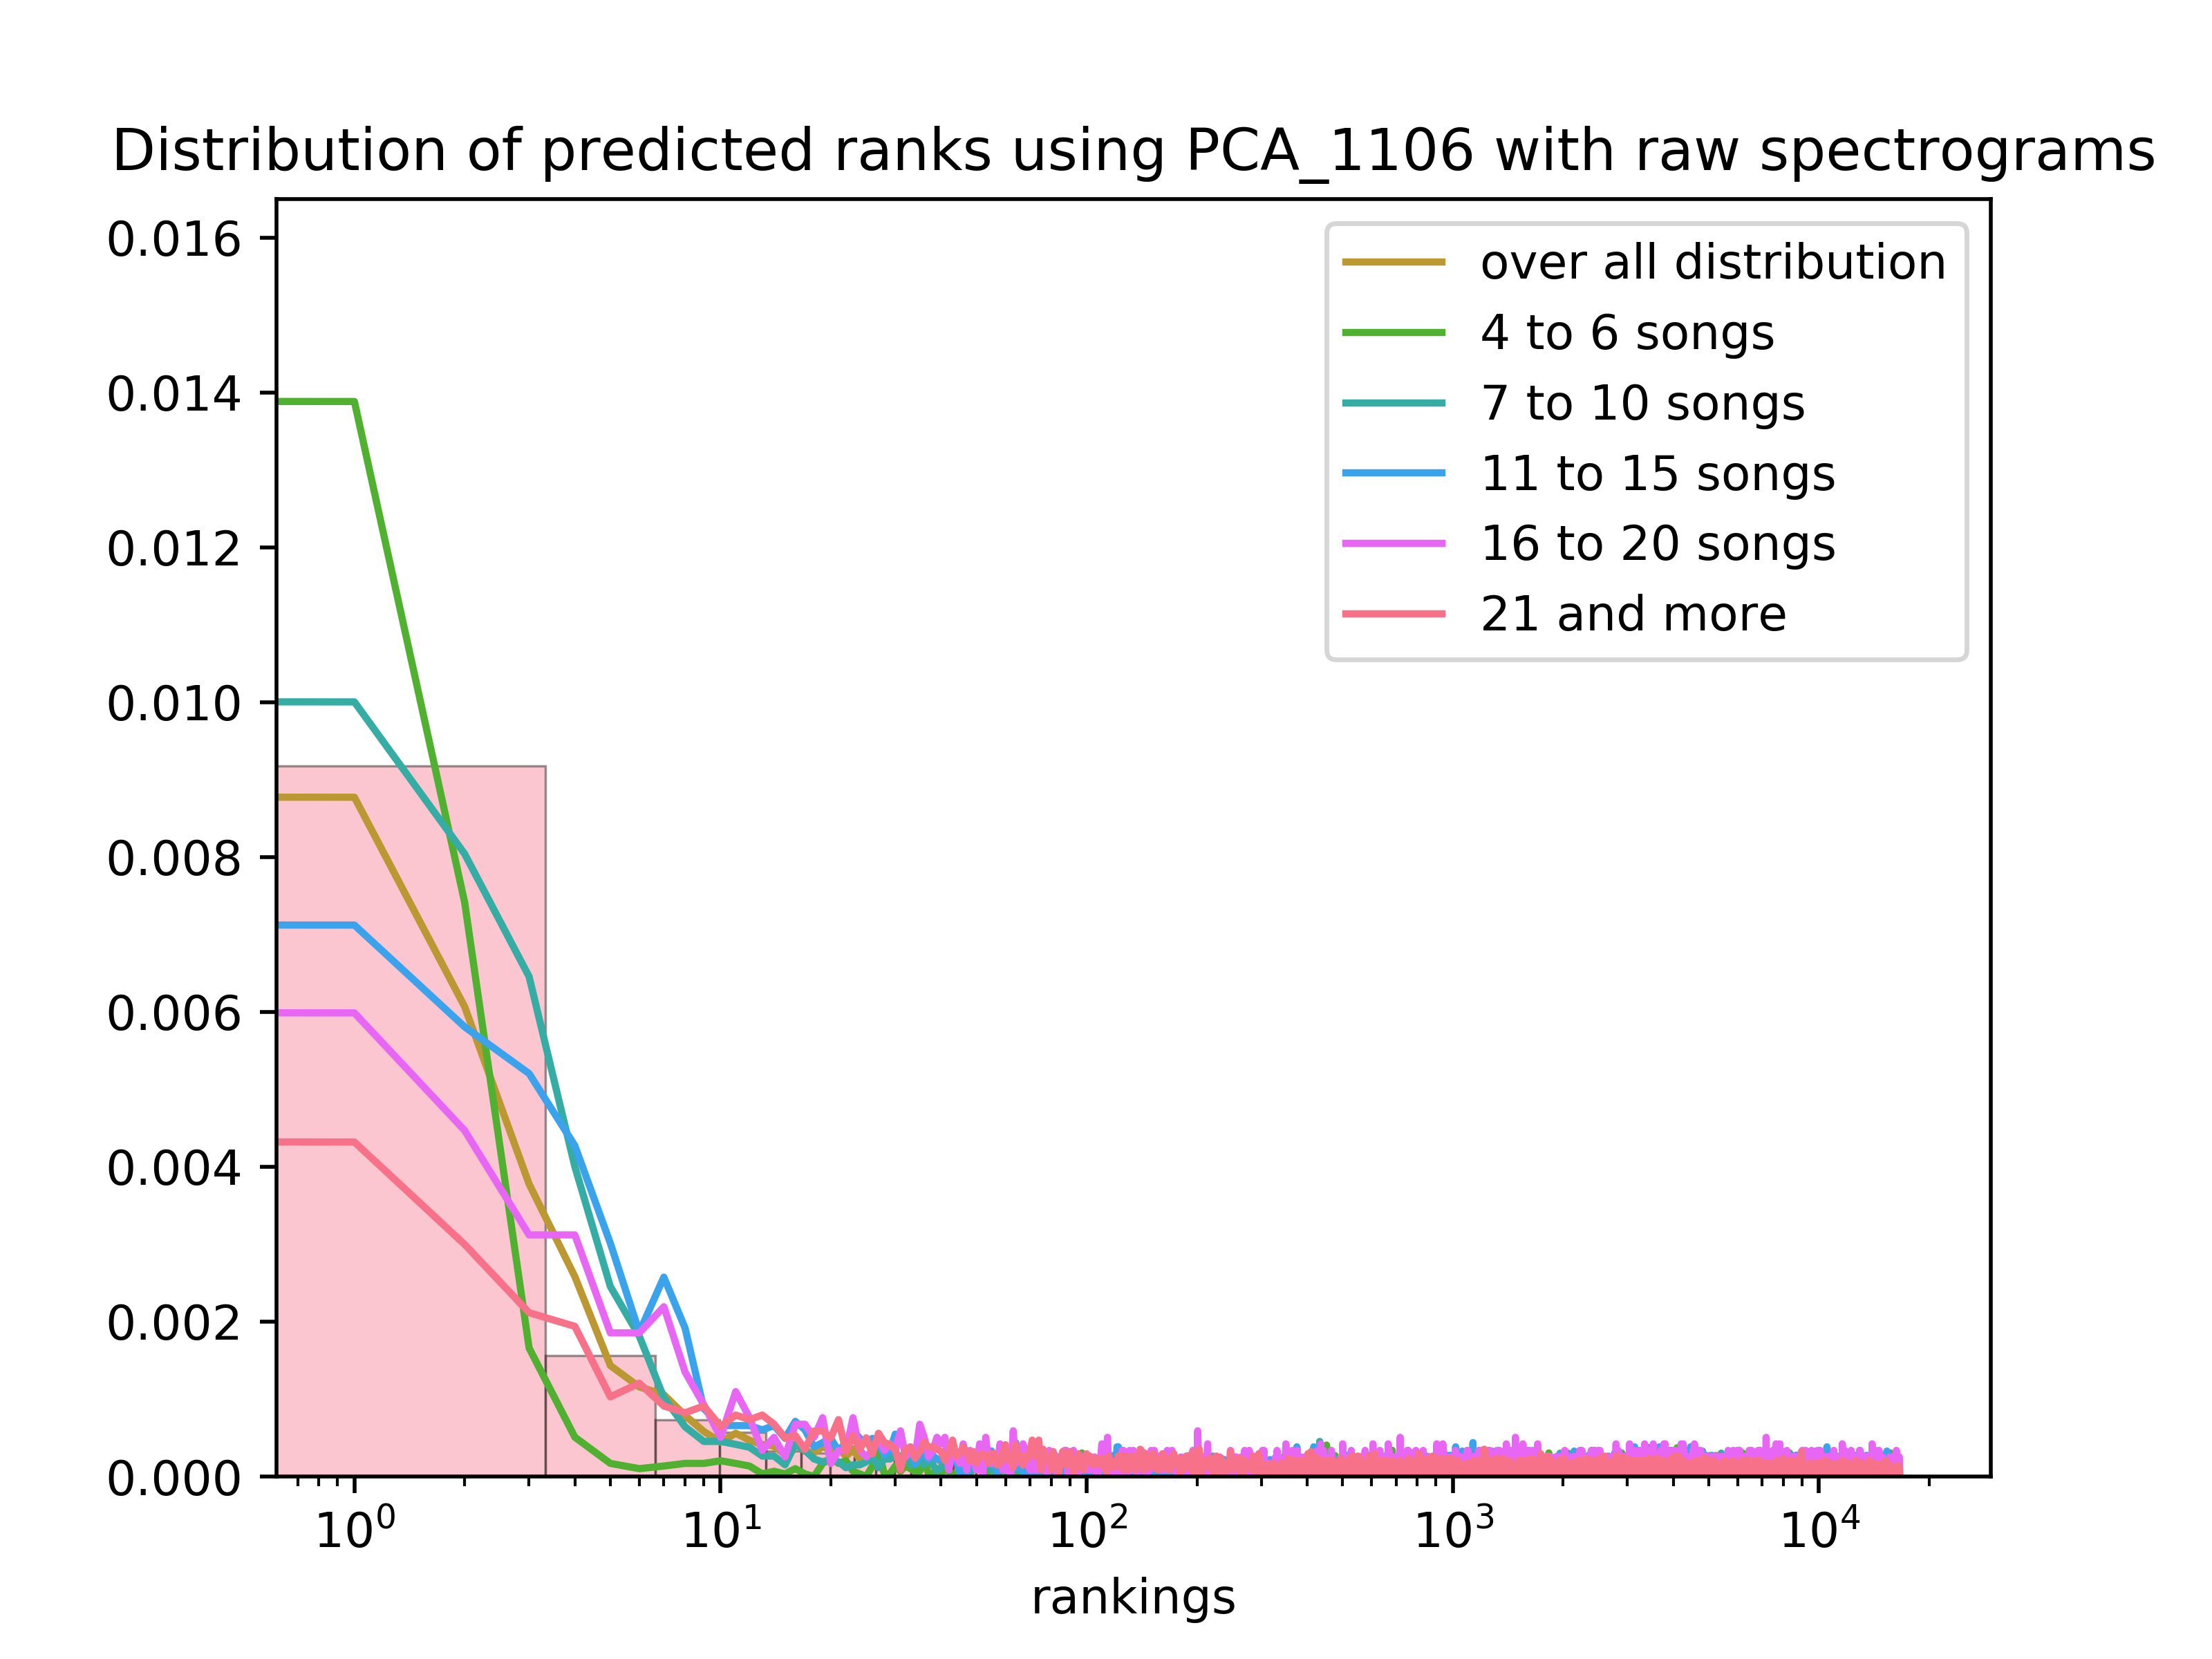
\includegraphics[width=1\linewidth]{./img/pca_spec_1106_graph.png}
  \caption[RDG of the PCA\_spec\_1106 method.]{RDG of the \newline PCA\_spec\_1106 method.}
  \label{fig:pca_spec_1106_distribution}
\end{minipage}
 \vspace{1cm}
\begin{minipage}{.45\textwidth}
  \centering
  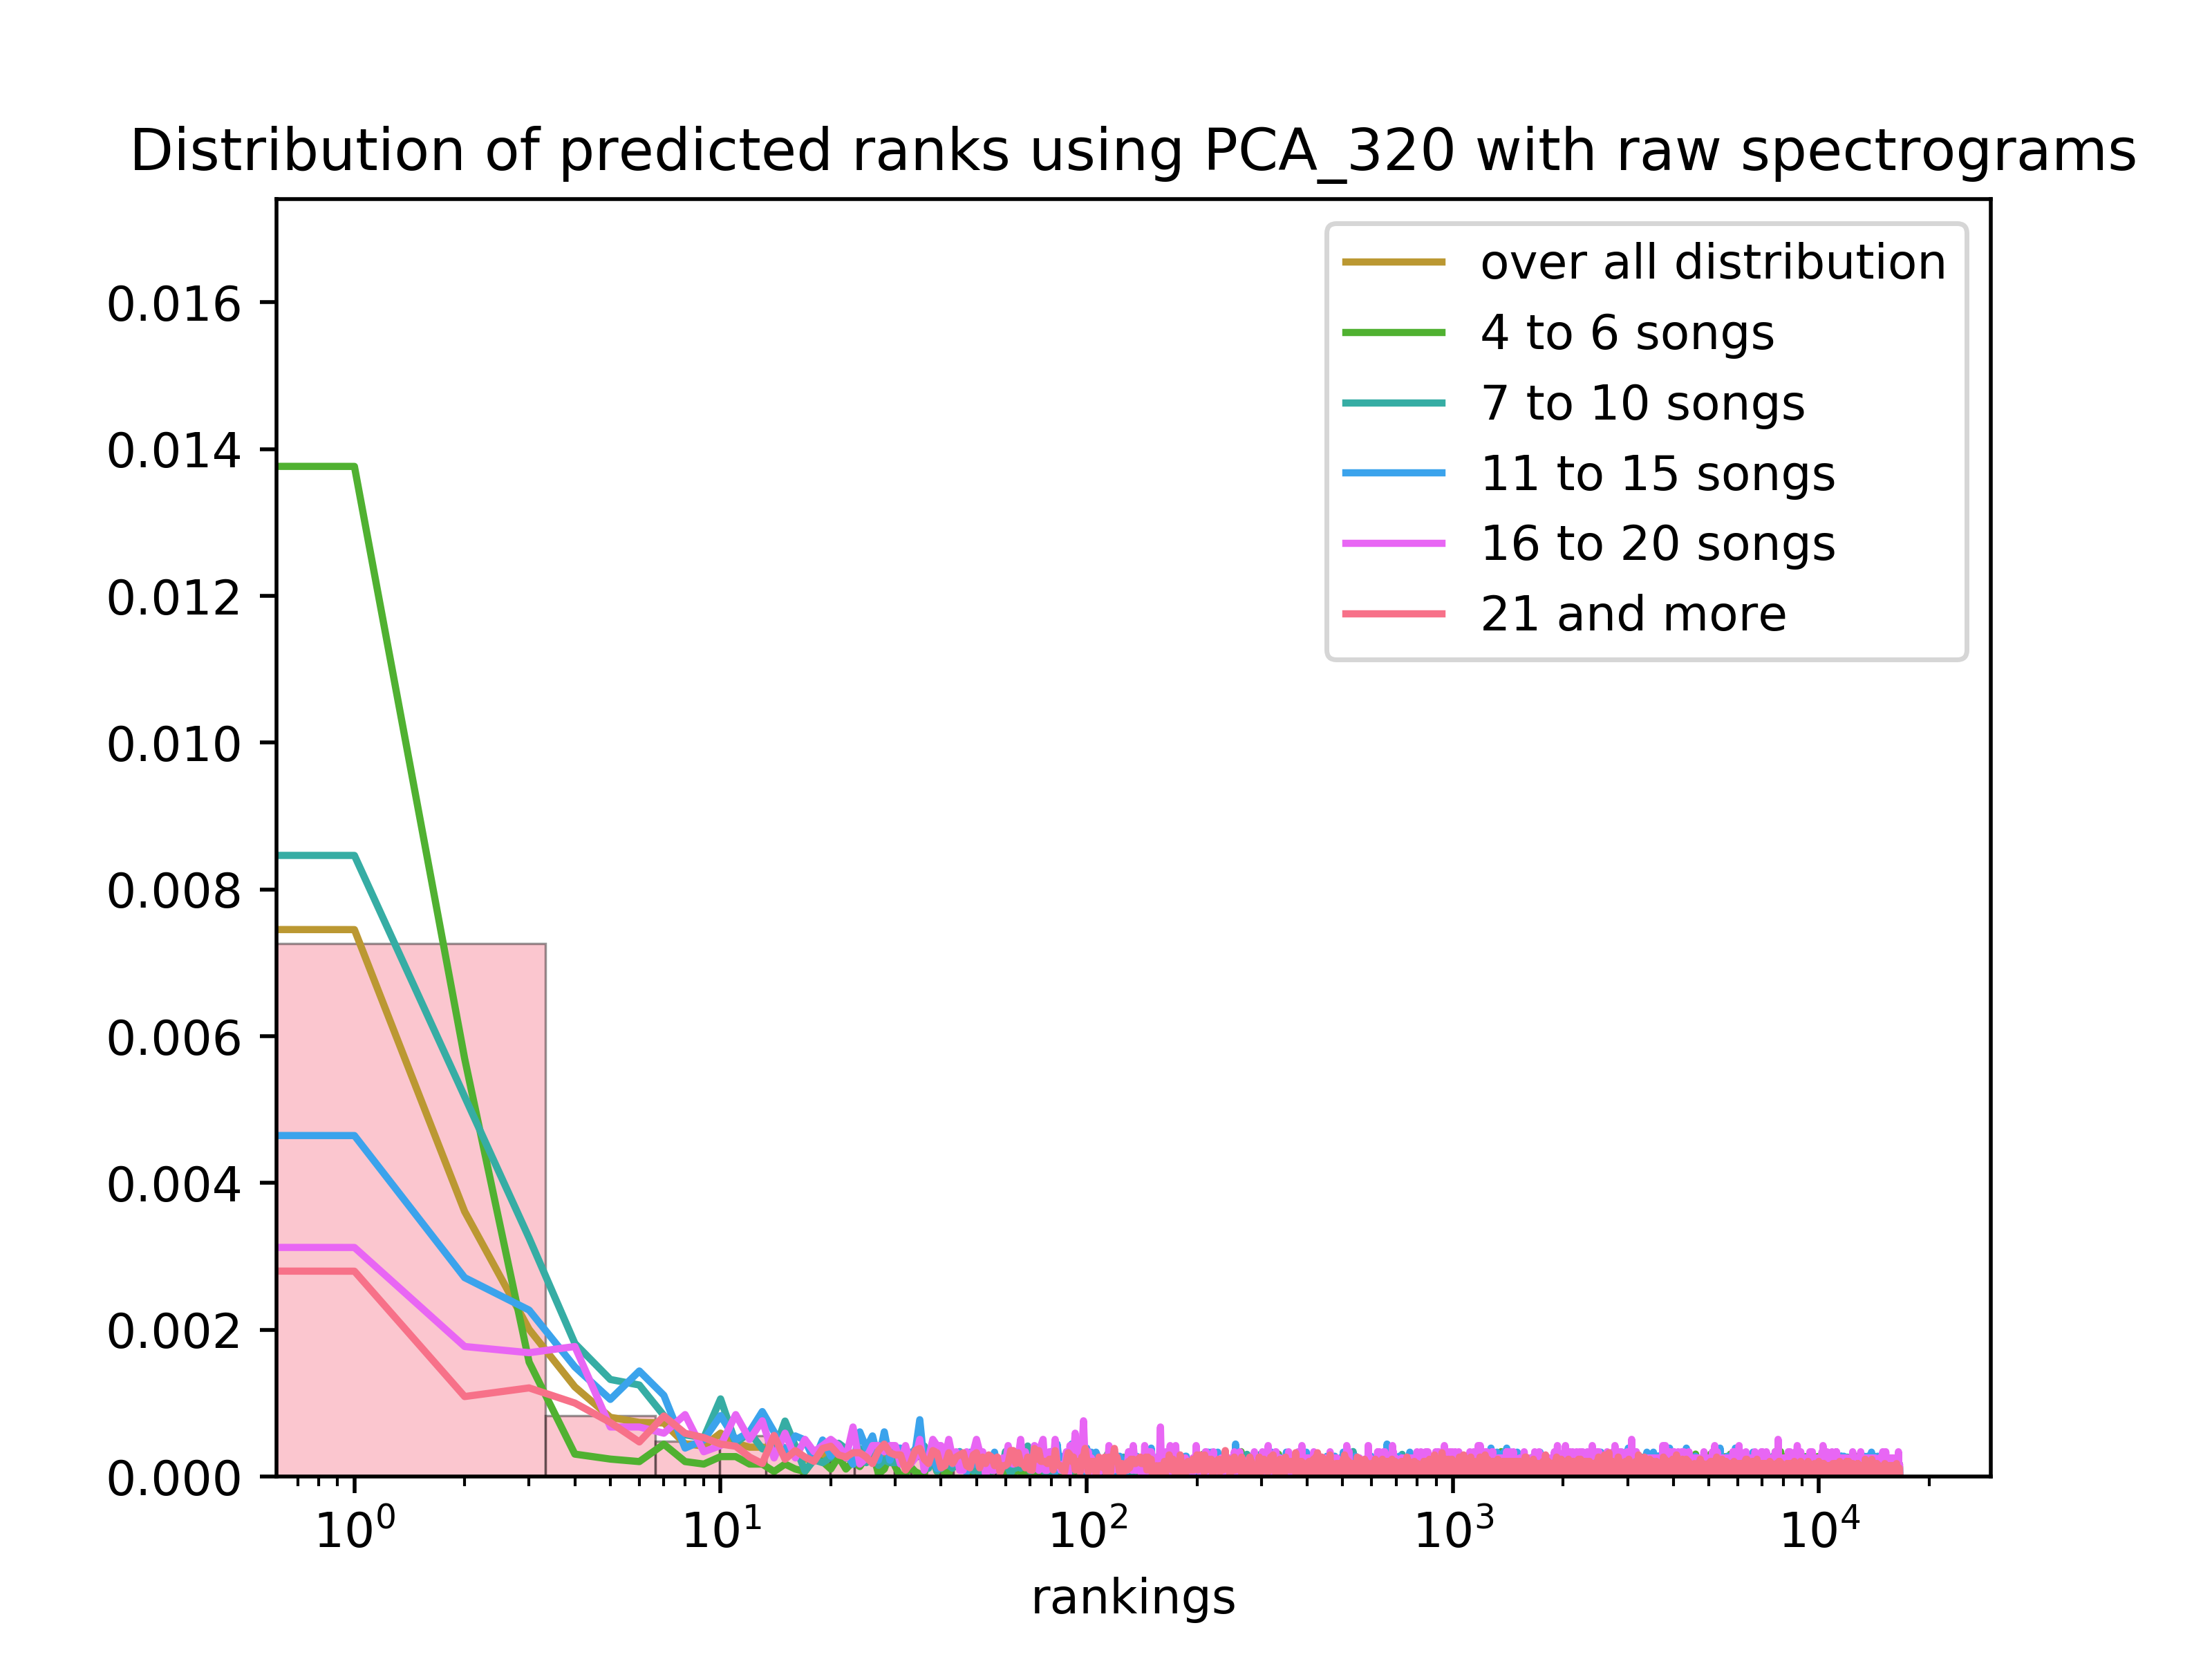
\includegraphics[width=1\linewidth]{./img/pca_spec_320_graph.png}
  \caption[RDG of the PCA\_spec\_320 method]{RDG of the \newline PCA\_spec\_320 method}
  \label{fig:pca_spec_320_distribution}
\end{minipage}
\end{figure}

\subsection{PCA on Mel-spectrograms}\label{ssec:pca_mel_results}

We had two PCA methods taking mel-spectrograms as input. The more radical dimension reduction did not lead to better performance. It actually worsened the results significantly and the PCA\_mel\_320 was our worse method. But only until we applied the threshold. For this method, the threshold improved the results over ten times. It is interesting because it was the PCA\_spec\_320 for which the results worsened after applying the threshold and one might think, that PCA methods with audio inputs will behave similarly.

Figure \ref{fig:pca_mel_5715_distribution} and Figure \ref{fig:pca_mel_320_distribution} illustrate the distributions for PCA\_mel\_5715 and PCA\_mel\_320. A thing to notice in the PCA\_mel\_{5715} RDG graph is that the number of the top 1-5 rankings for longer playlists is not quite as low compared to the other methods we tested. We still observe the trend of a considerably higher number of the top 1-5 ranks for shorter playlists, however, it is not as significant as for example for raw mel-spectrograms.
\begin{figure}[h]
\centering
\begin{minipage}{.45\textwidth}
  \centering
  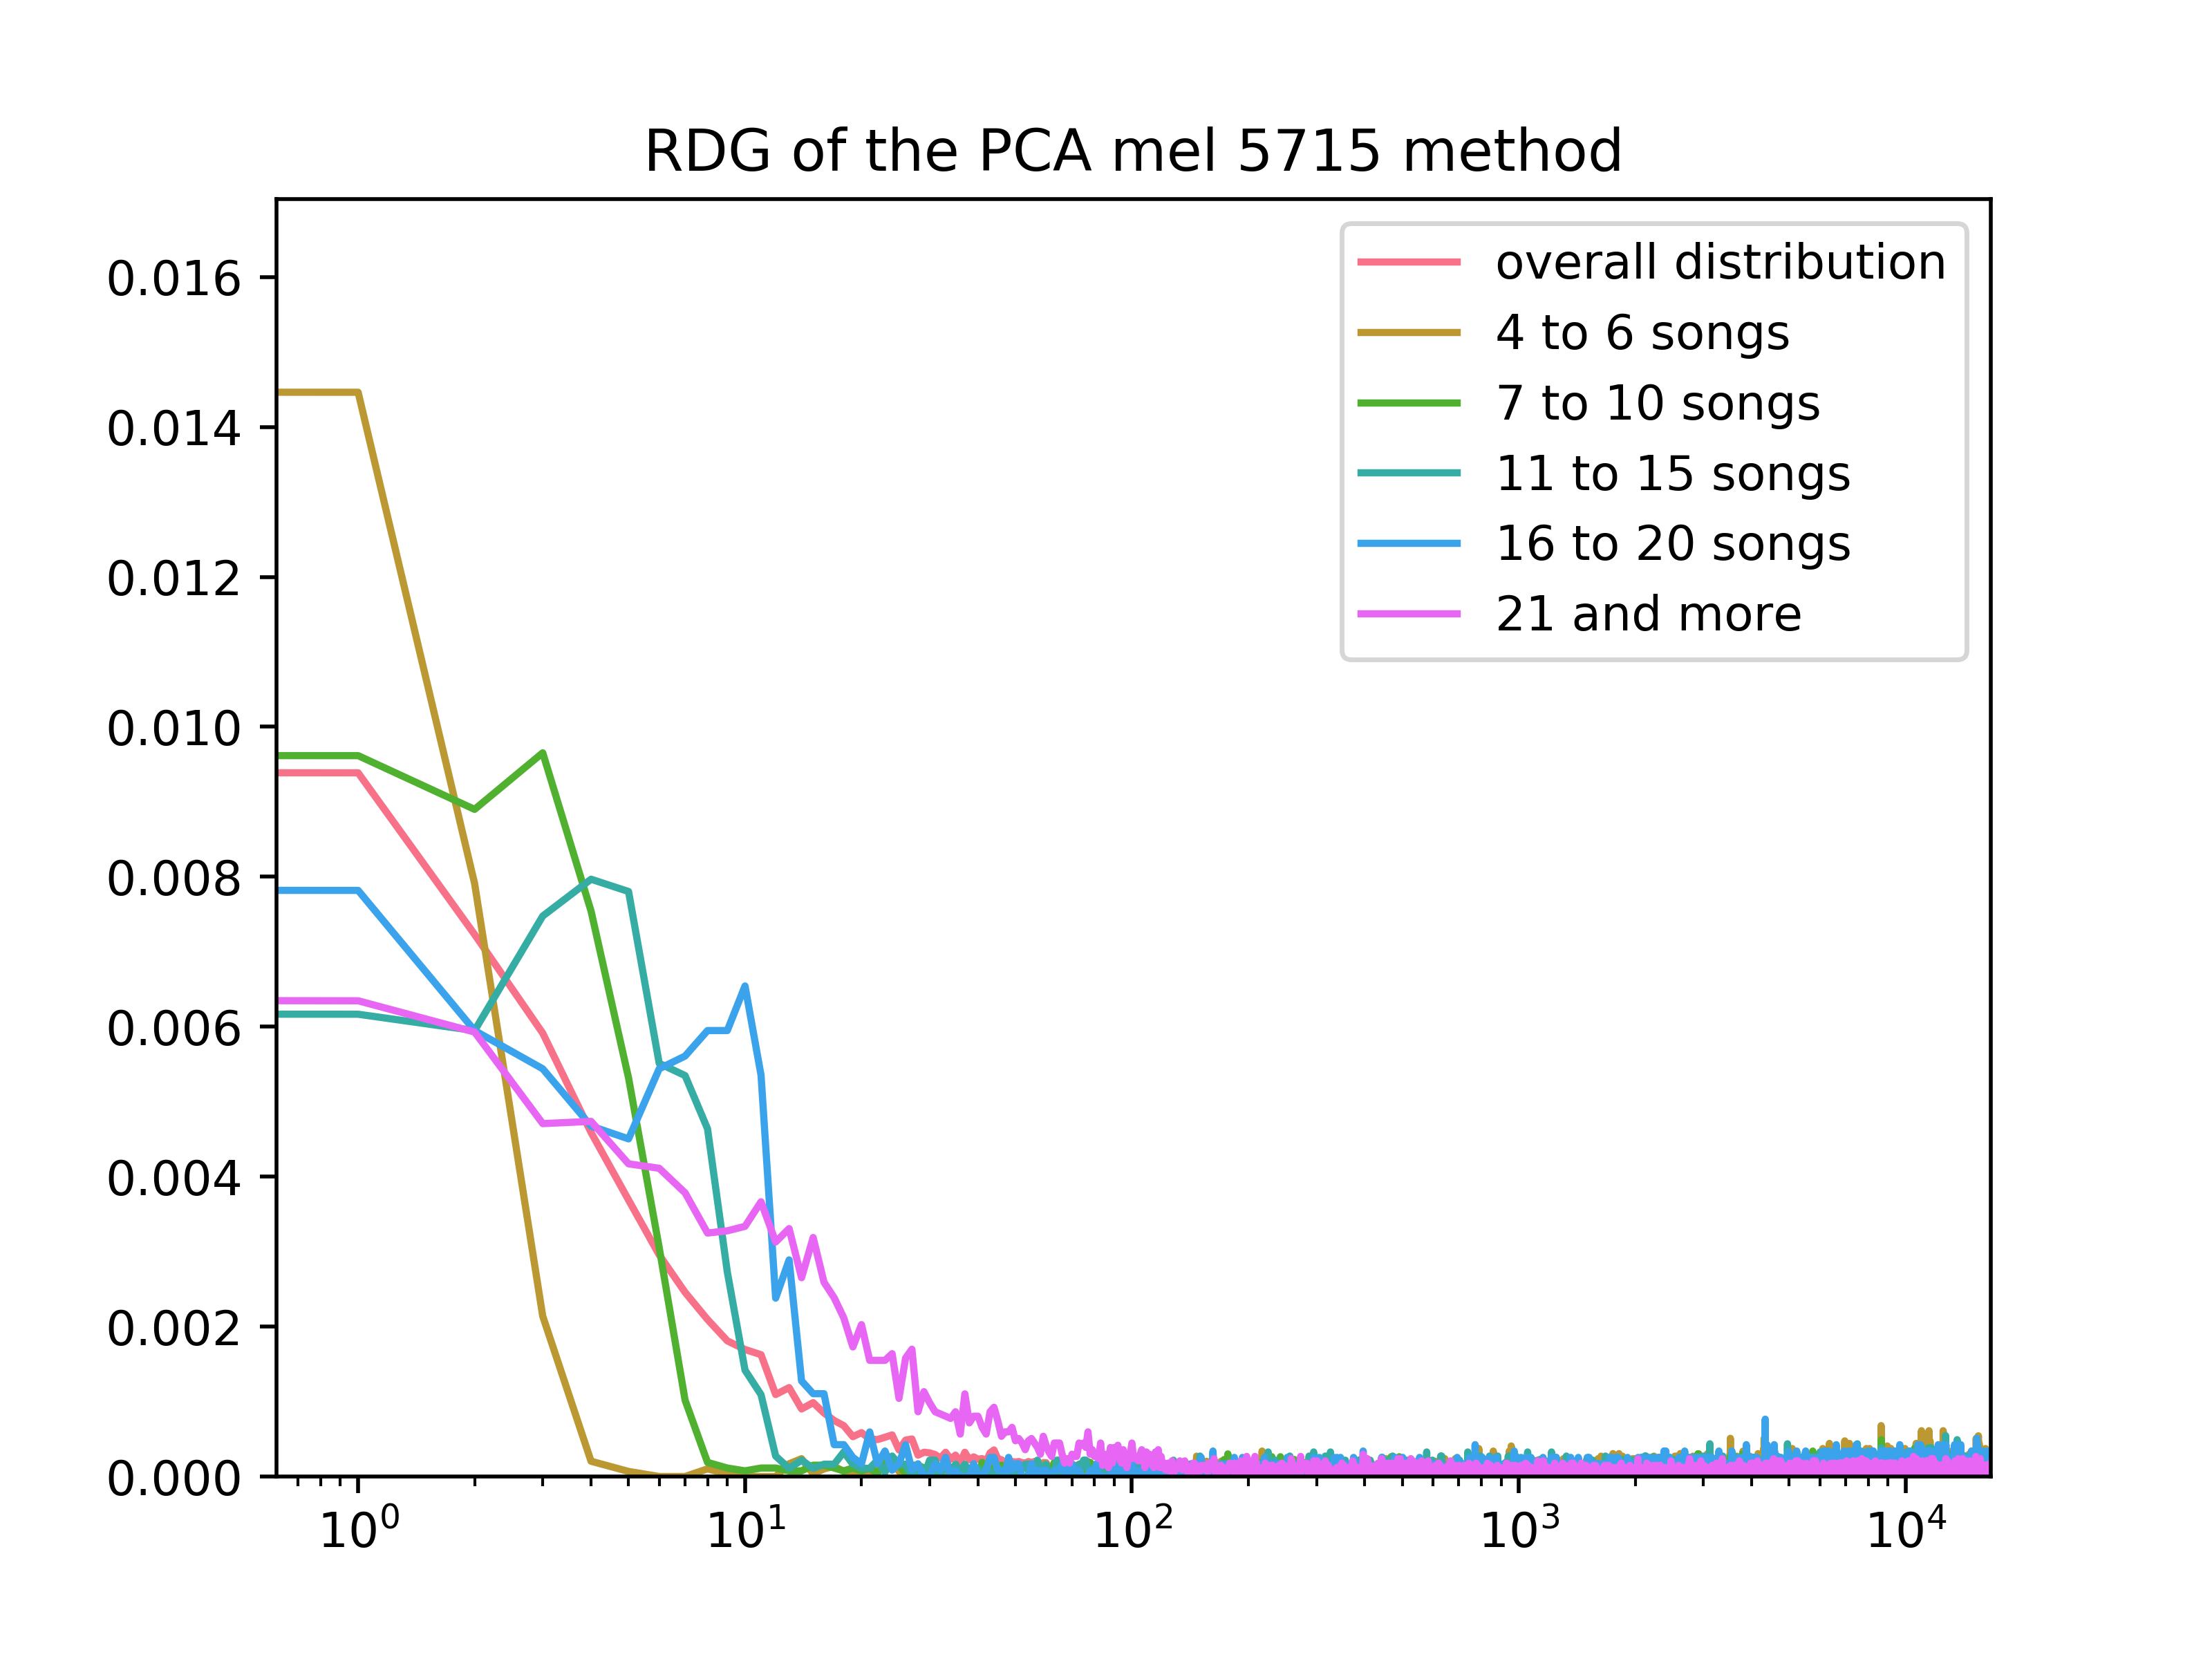
\includegraphics[width=1\linewidth]{./img/pca_mel_5715_graph.png}
  \caption[RDG of the PCA\_mel\_5712]{RDG of the \newline PCA\_mel\_5712.}
  \label{fig:pca_mel_5715_distribution}
\end{minipage}
 \vspace{1cm}
\begin{minipage}{.45\textwidth}
  \centering
  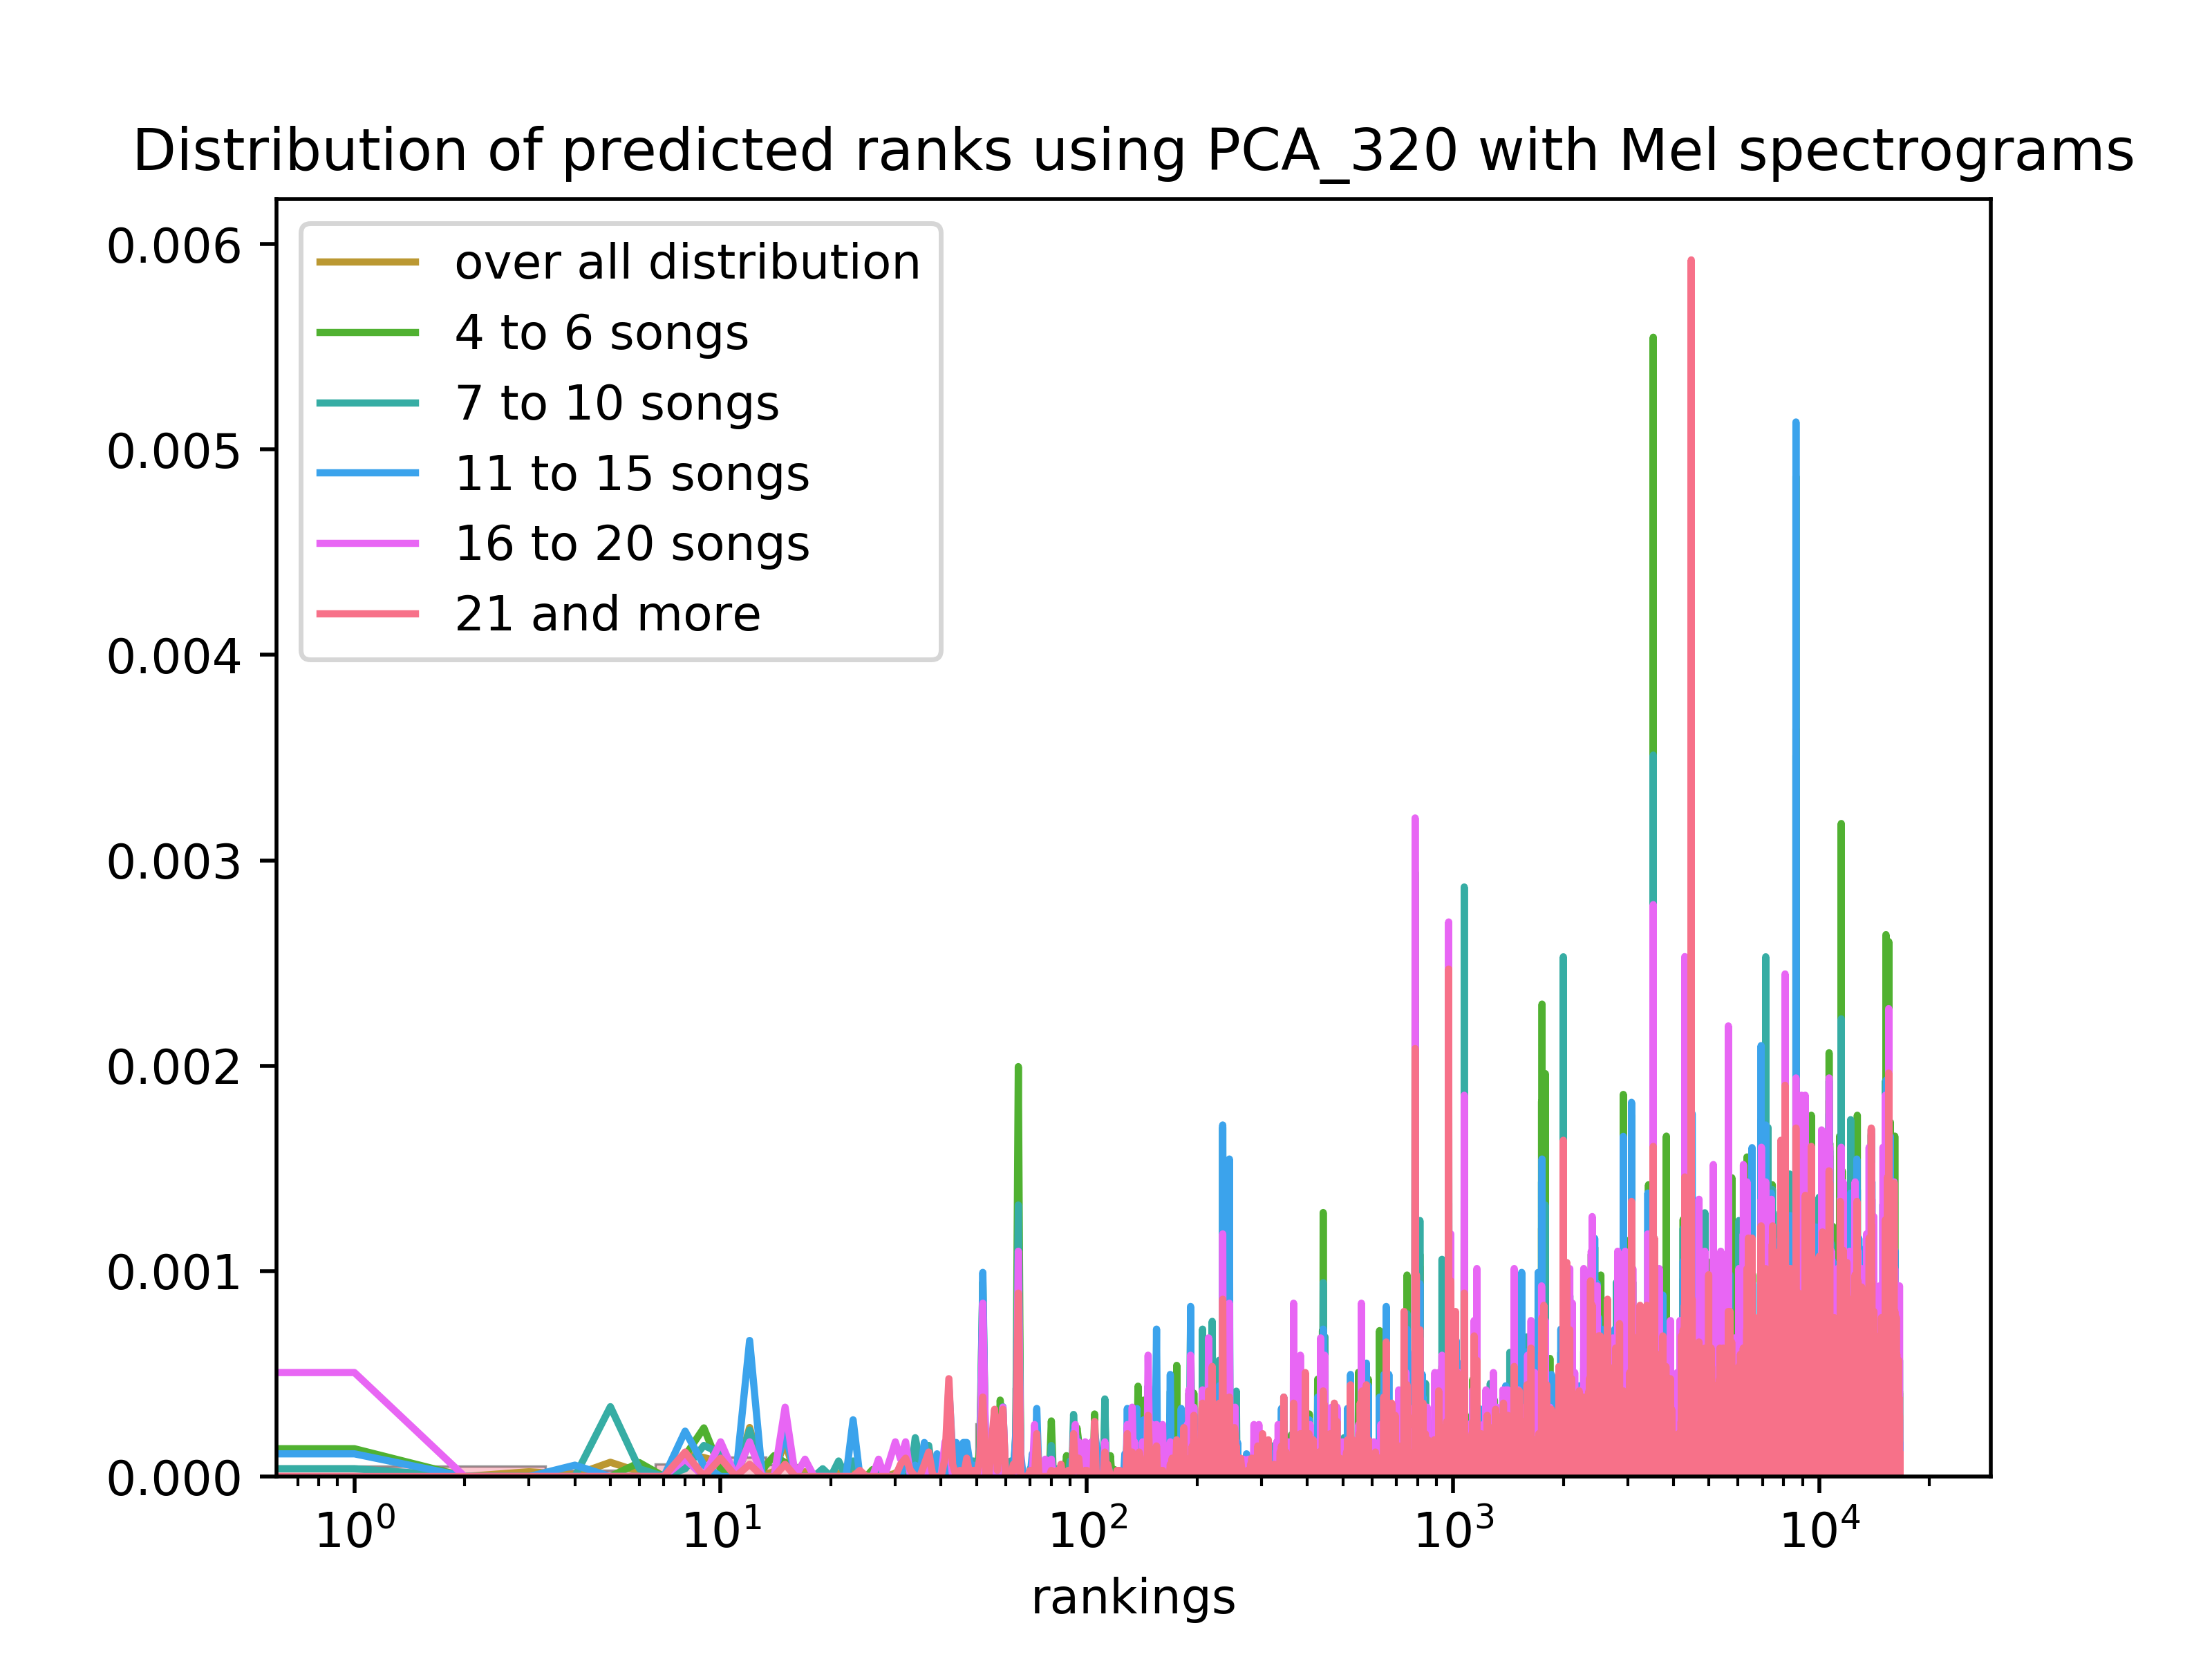
\includegraphics[width=1\linewidth]{./img/pca_mel_320_graph.png}
  \caption[RDG of the PCA\_mel\_320 method]{RDG of the \newline PCA\_mel\_320 method.}
  \label{fig:pca_mel_320_distribution}
\end{minipage}
\end{figure}\label{fig:pca_mel_comparison_graps}

\section{Deep audio representation results}\label{sec:deep_audio_results}

\subsection{GRU network with spectrogram input}\label{ssec:gru_spec_results}

As can be observed in Figure \ref{fig:all_model_training} the training loss is basically constant for both GRU networks with spectrogram input (the GRU\_spec\_20400 is hidden behind the orange line of GRU\_spec\_5712 as their progress or rather the lack of it is the same). This means, that the network did not really learn. Therefore it is not suprising that the GRU\_spec\_5712 does not rank among the best. And it is quite surprising, that the GRU\_spec\_20400, even though it appeared to be quite bad before the application of the threshold, improved with defining similarity with the threshold and became the best method with spectrogram input as can be seen in Table \ref{table:spec_methods}. The table shows that 4.3\% of songs were ranked in the top 10, 5.2\% in the top 50 and 5.7\% in the top 100 for the longer GRU spectrogram model. For the short GRU spectrogram model, the results are significantly worse with 0.2\% for the top ten songs 0.6\% ranked in the top 50 and a little over 1\% ranked in the top 100. 

The RDGs depicted in Figures \ref{fig:gru_spec_20400_distribution} and \ref{fig:gru_spec_5712_distribution} of both GRU\_specs is are dissimilar too. The overall trend for the short playlist drop and stability of long playlists is visible in the graph for GRU\_spec\_20400 but not in the graph for GRU\_spec\_5712 where there is a trace of it but the values seem to be quite random so it fades. 

\begin{figure}[h]
\centering
\begin{minipage}{.45\textwidth}
  \centering
  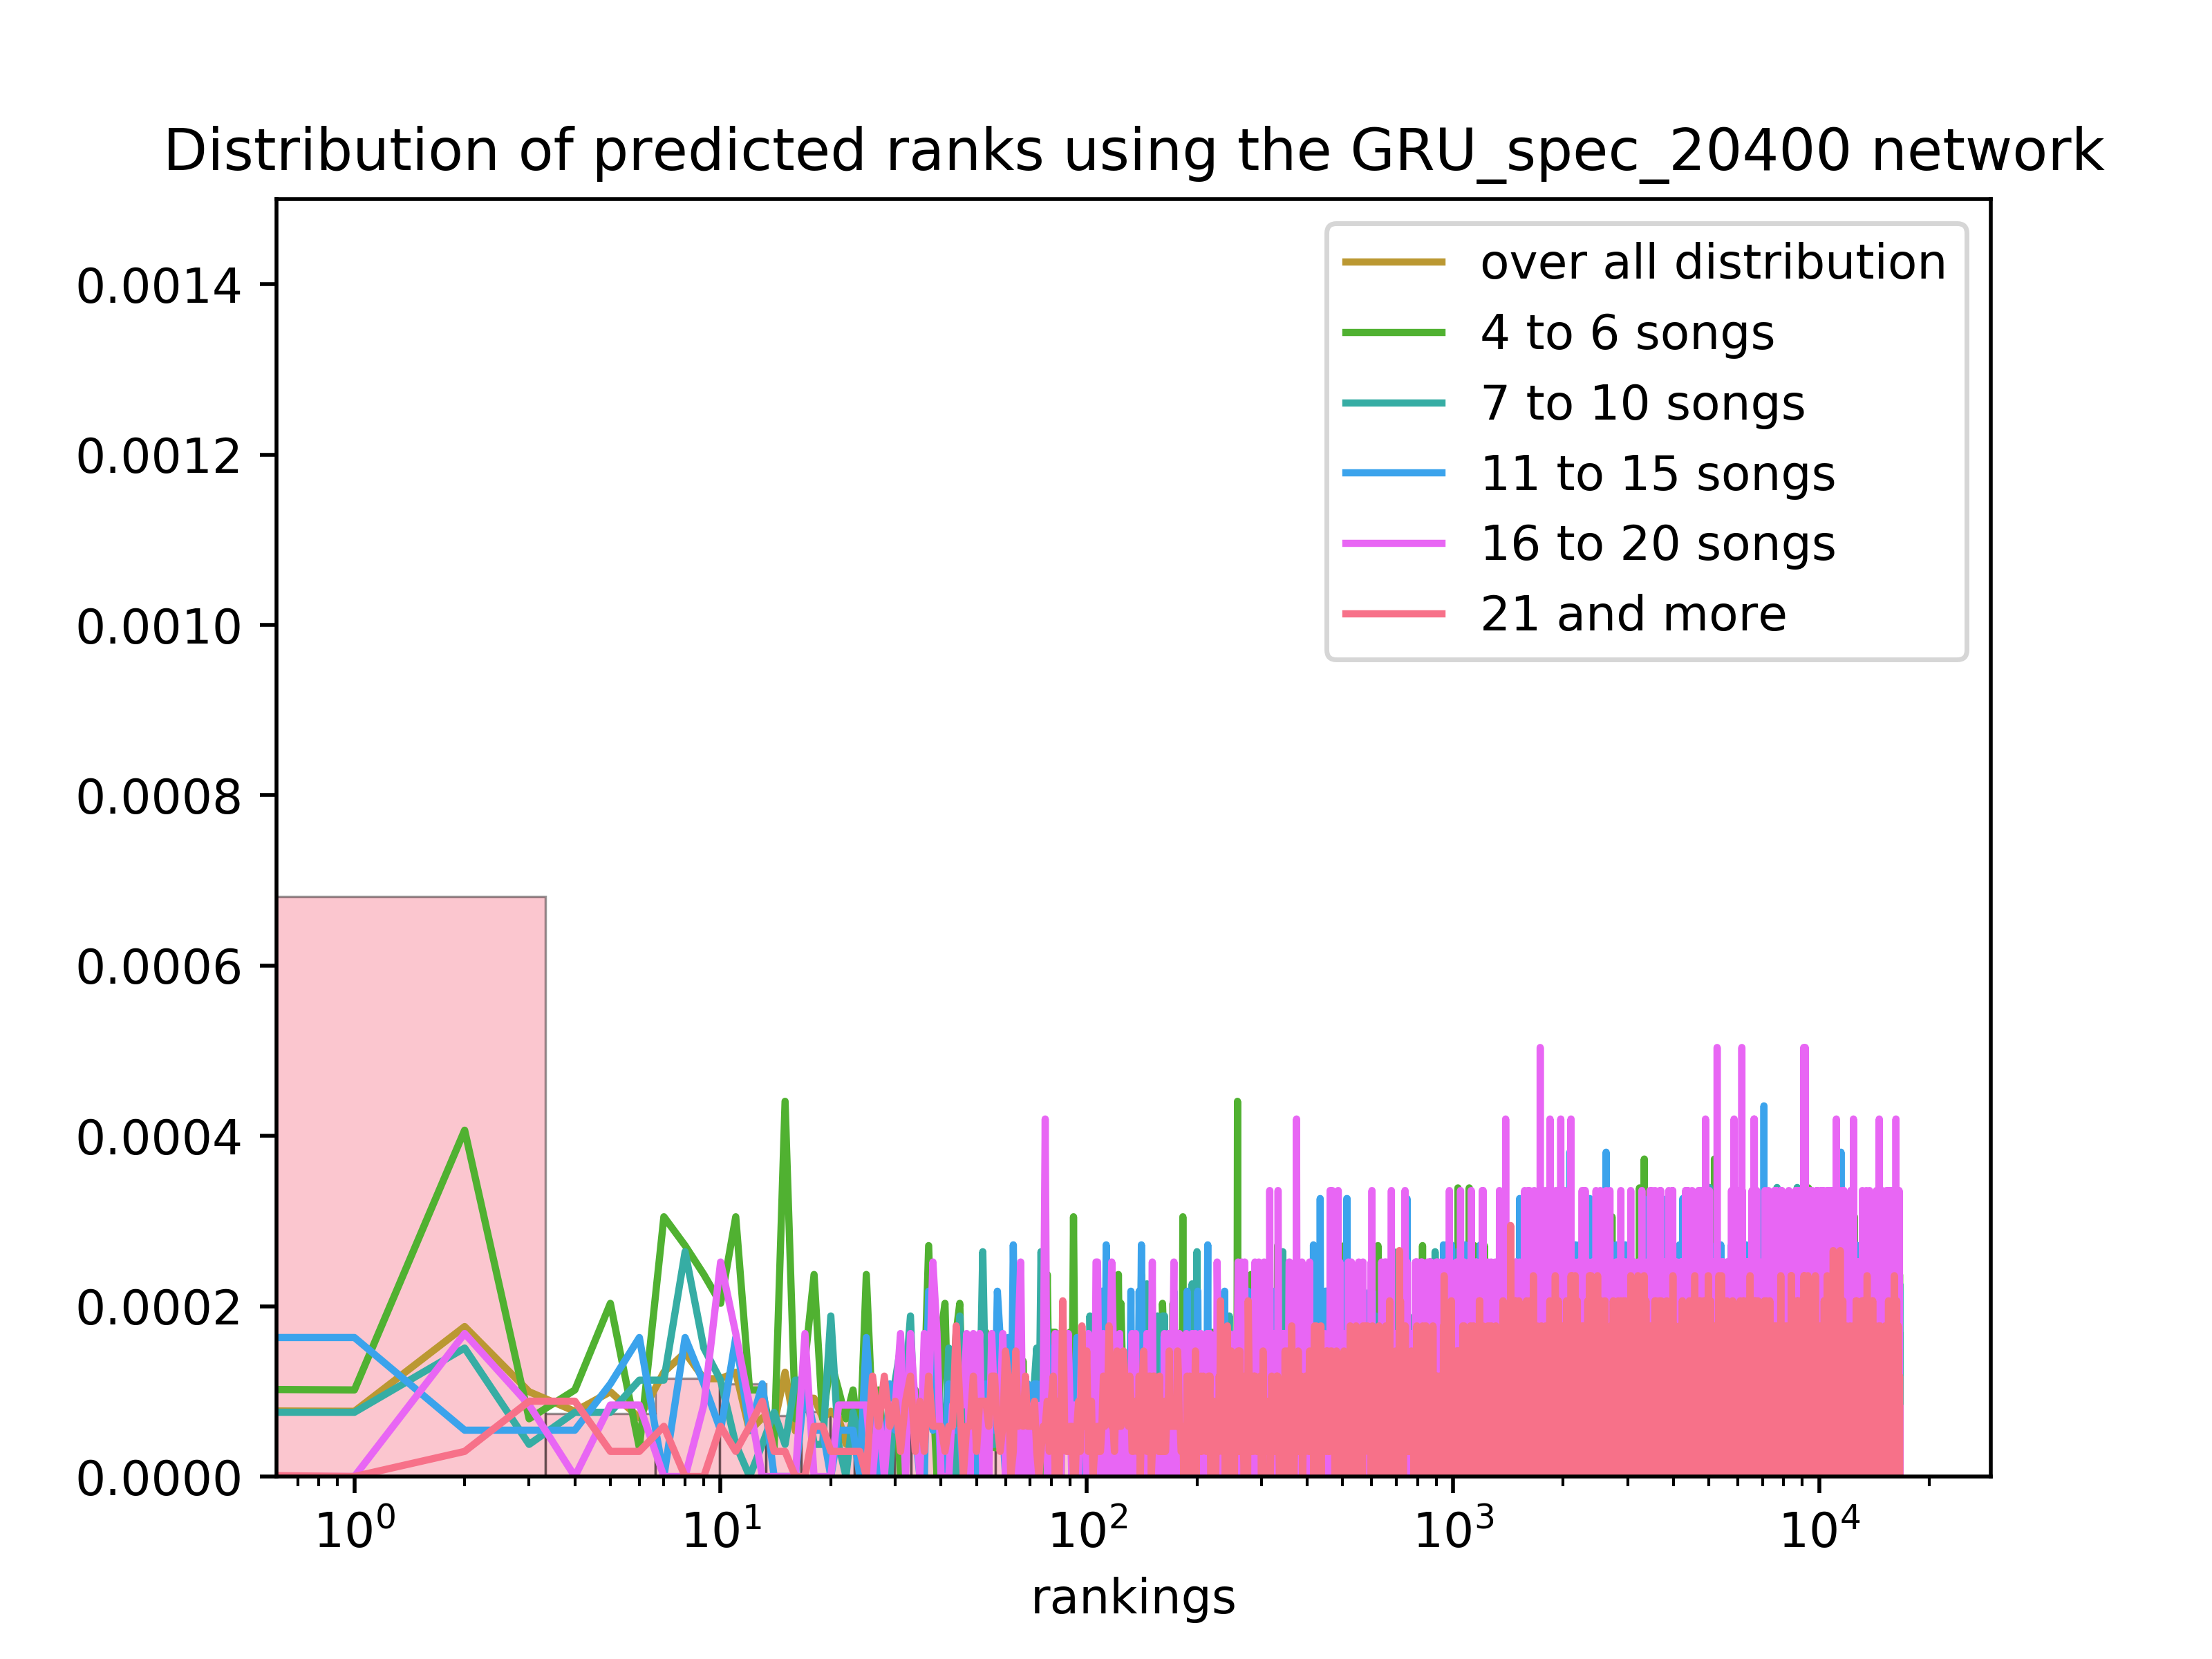
\includegraphics[width=1\linewidth]{./img/gru_spec_20400_graph.png}
  \caption[RDG of the GRU\_spec\_20400 method]{RDG of the \newline GRU\_spec\_20400 method.}
  \label{fig:gru_spec_20400_distribution}
\end{minipage}
 \vspace{1cm}
\begin{minipage}{.45\textwidth}
  \centering
  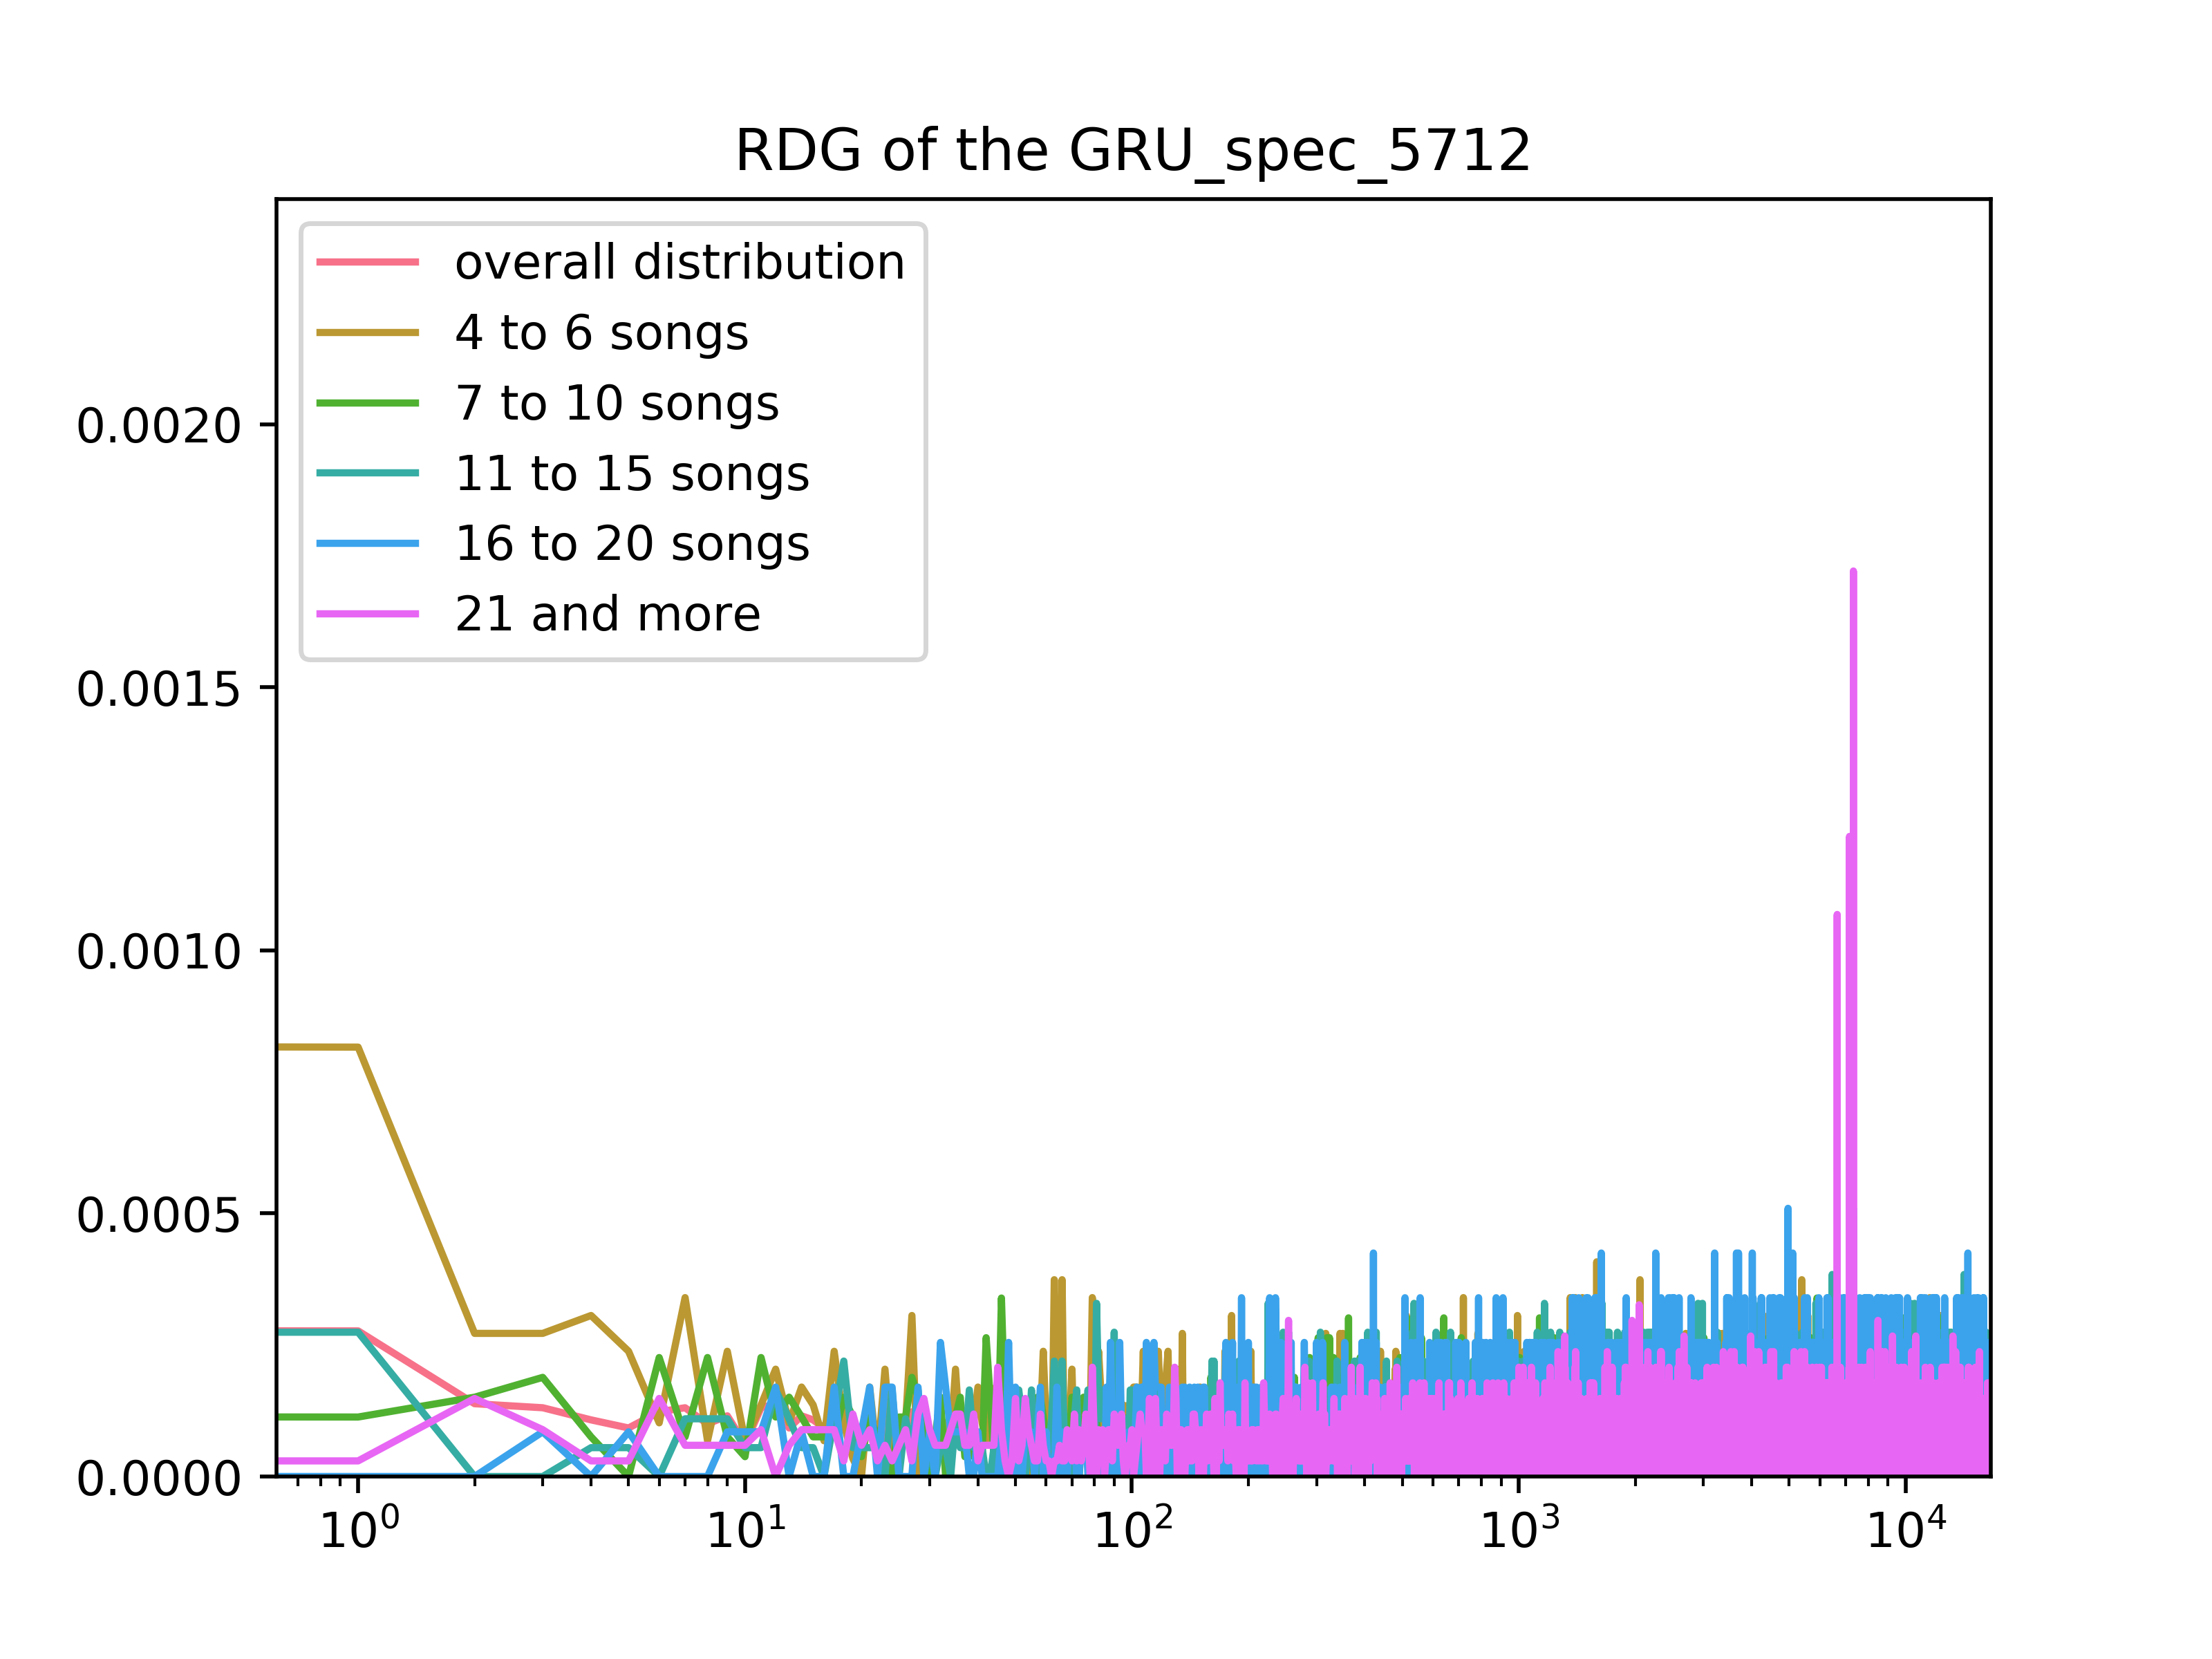
\includegraphics[width=1\linewidth]{./img/gru_spec_5712_graph.png}
  \caption[RDG of the GRU\_spec\_5712 method]{RDG of the \newline GRU\_spec\_5712 method.}
  \label{fig:gru_spec_5712_distribution}
\end{minipage}
\end{figure}\label{fig:gru_spec_distributions}

\subsection{LSTM network with spectrogram input}\label{ssec:LSTM_spec_results}

Unlike the GRU model training which showed almost no improvement even after 100 epochs of training, the LSTM\_specs as one can observe in Figure \ref{fig:all_model_training} where the LSTM\_spec\_20400 is rendered in green and the LSTM\_spec\_5712 in red went through progress. The decrease of training loss slowed down significantly towards the end of the 100 epochs.

The bigger improvement of the training loss correlated with better results for the LSTM\_spec methods. But only until we applied the threshold. It raised performance of all methods but the boost for GRU\_spec\_20400 was so big that it vaulted over both LSTM methods. In Table \ref{table:spec_methods} are the results of both LSTM\_spec models. 

A thing worth noting is that the LSTM\_spec method with bigger dimension reduction had worse results even before applying the threshold. And it stayed that way even after the threshold similarity as we can see in Table \ref{table:spec_methods} and in Figures \ref{fig:lstm_spec_20400_distribution} and \ref{fig:lstm_spec_5712_distribution} which visualize the difference between the two LSTM\_spec methods.

\begin{figure}[h]
\centering
\begin{minipage}{.45\textwidth}
  \centering
  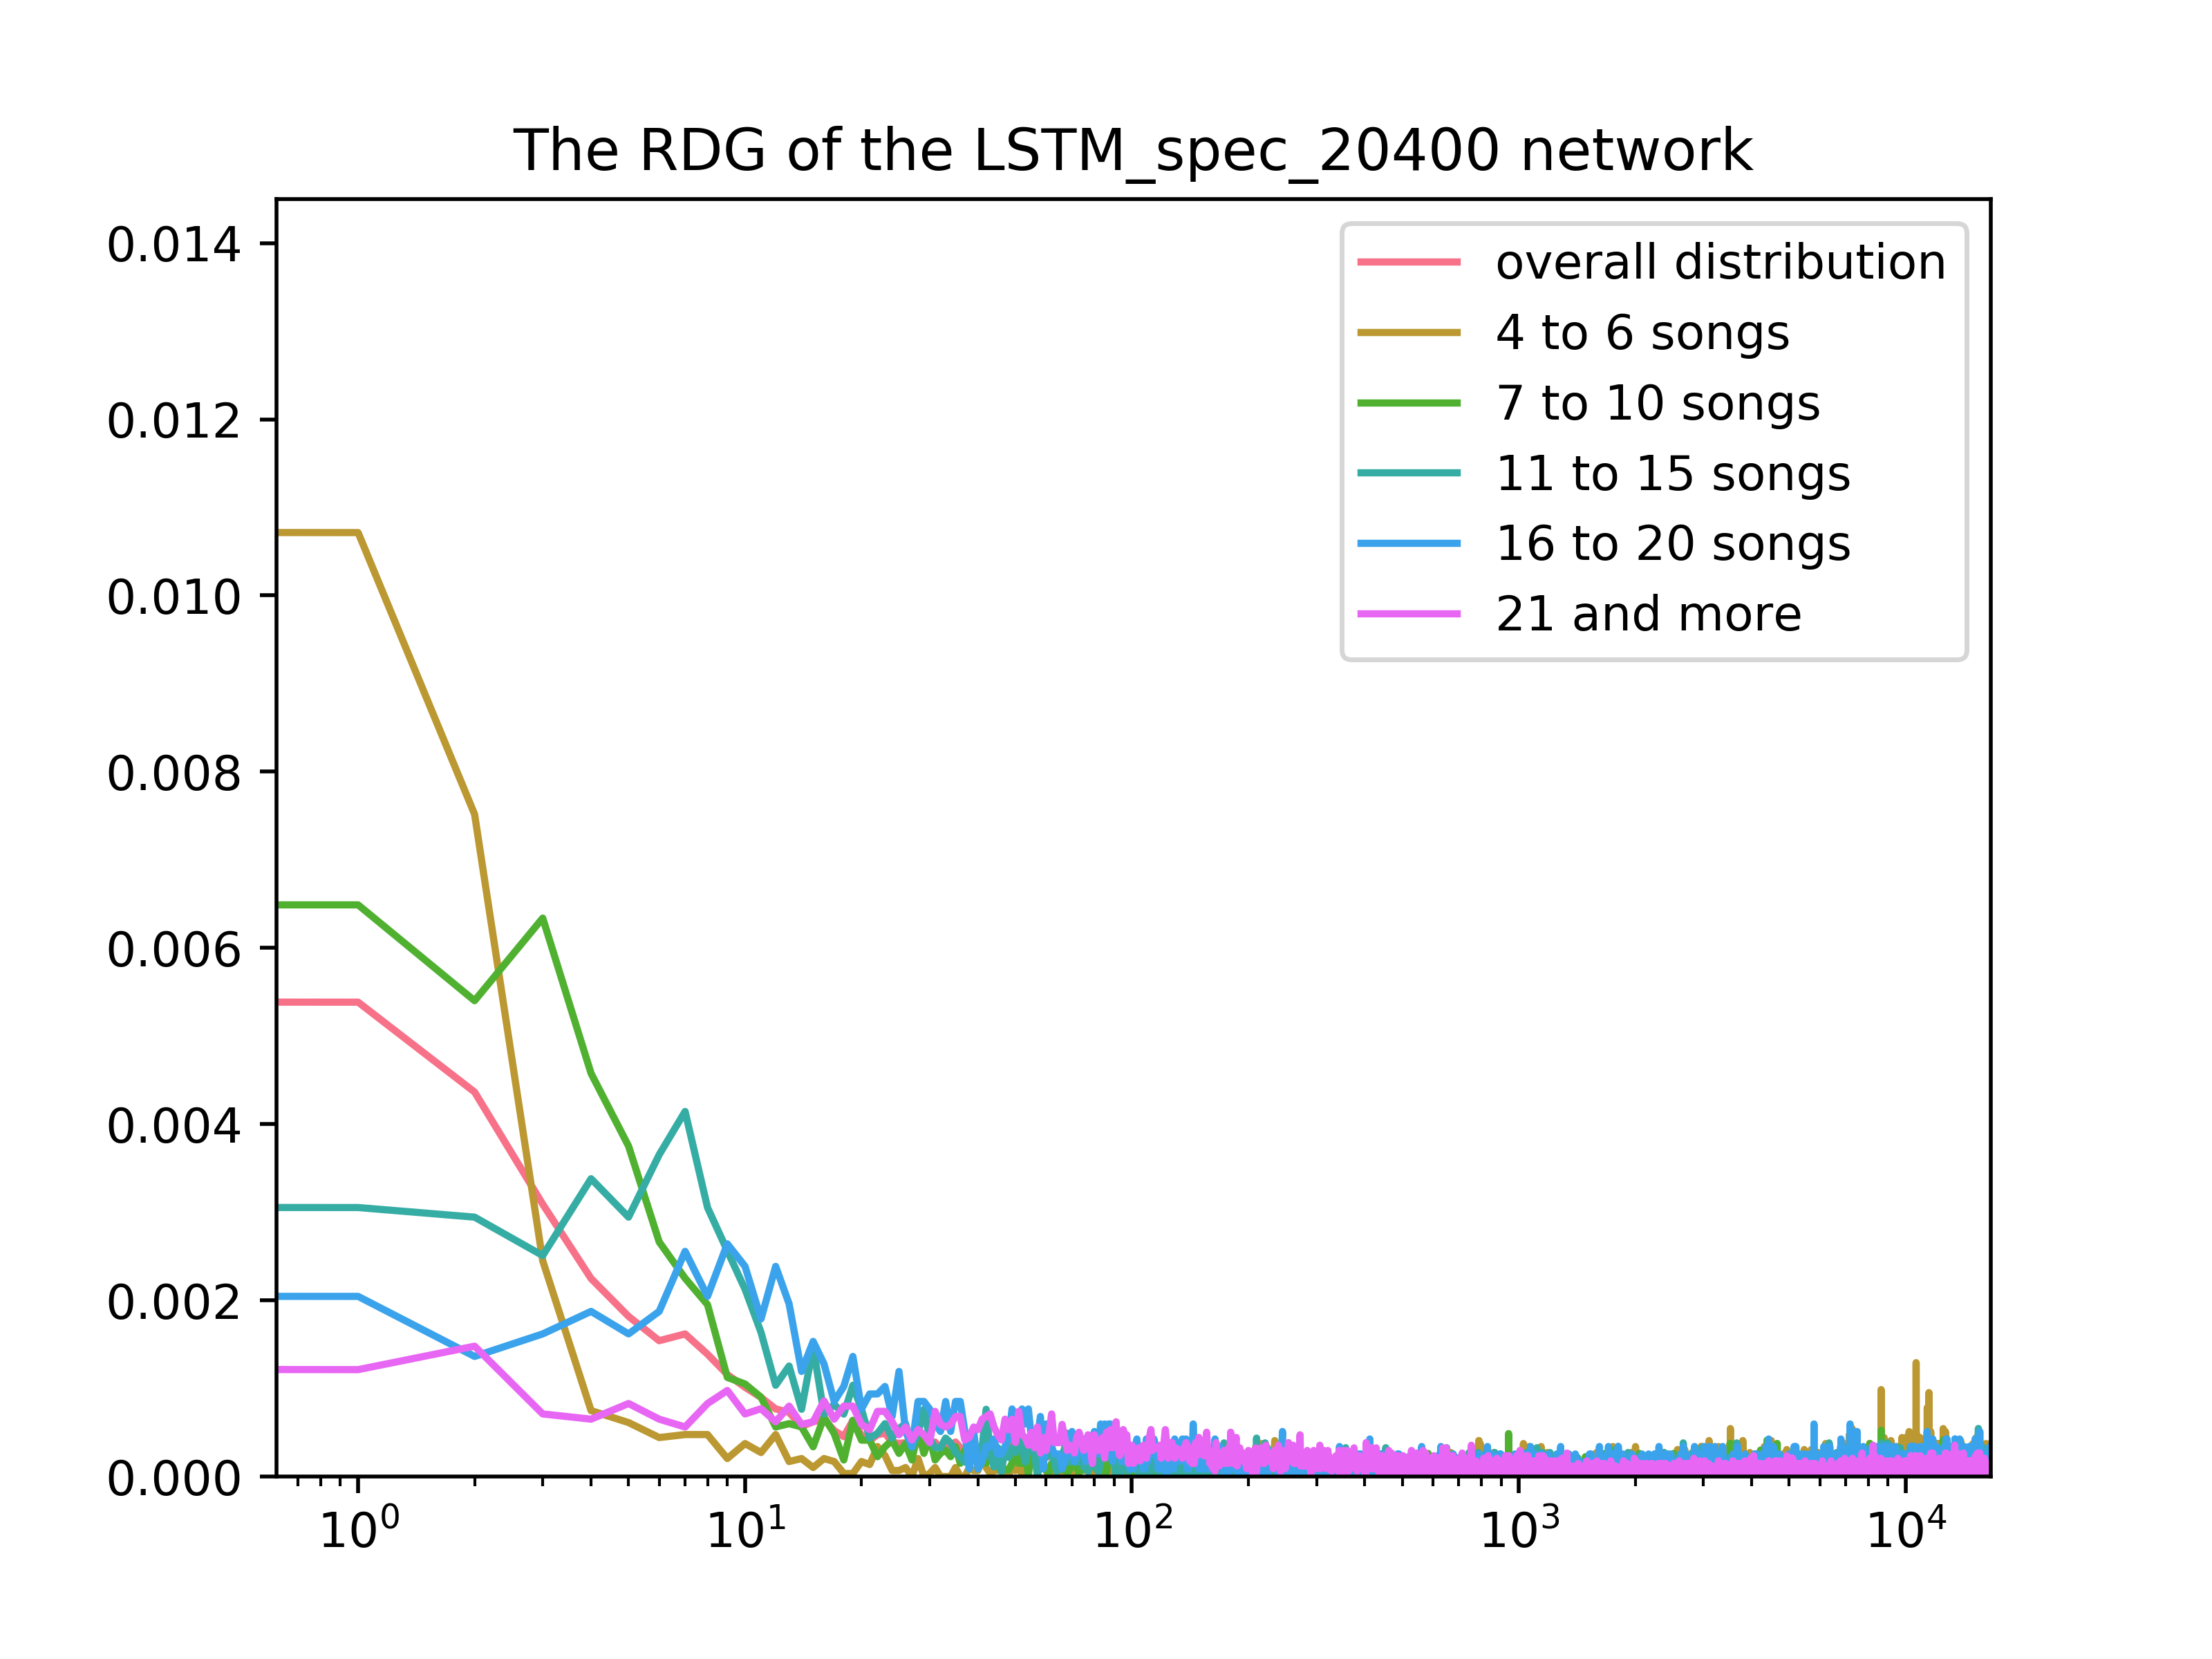
\includegraphics[width=1\linewidth]{./img/lstm_spec_20400_graph.png}
  \caption[RDG of the LSTM\_spec\_20400 method]{RDG of the \newline LSTM\_spec\_20400 method.}
  \label{fig:lstm_spec_20400_distribution}
\end{minipage}
 \vspace{1cm}
\begin{minipage}{.45\textwidth}
  \centering
  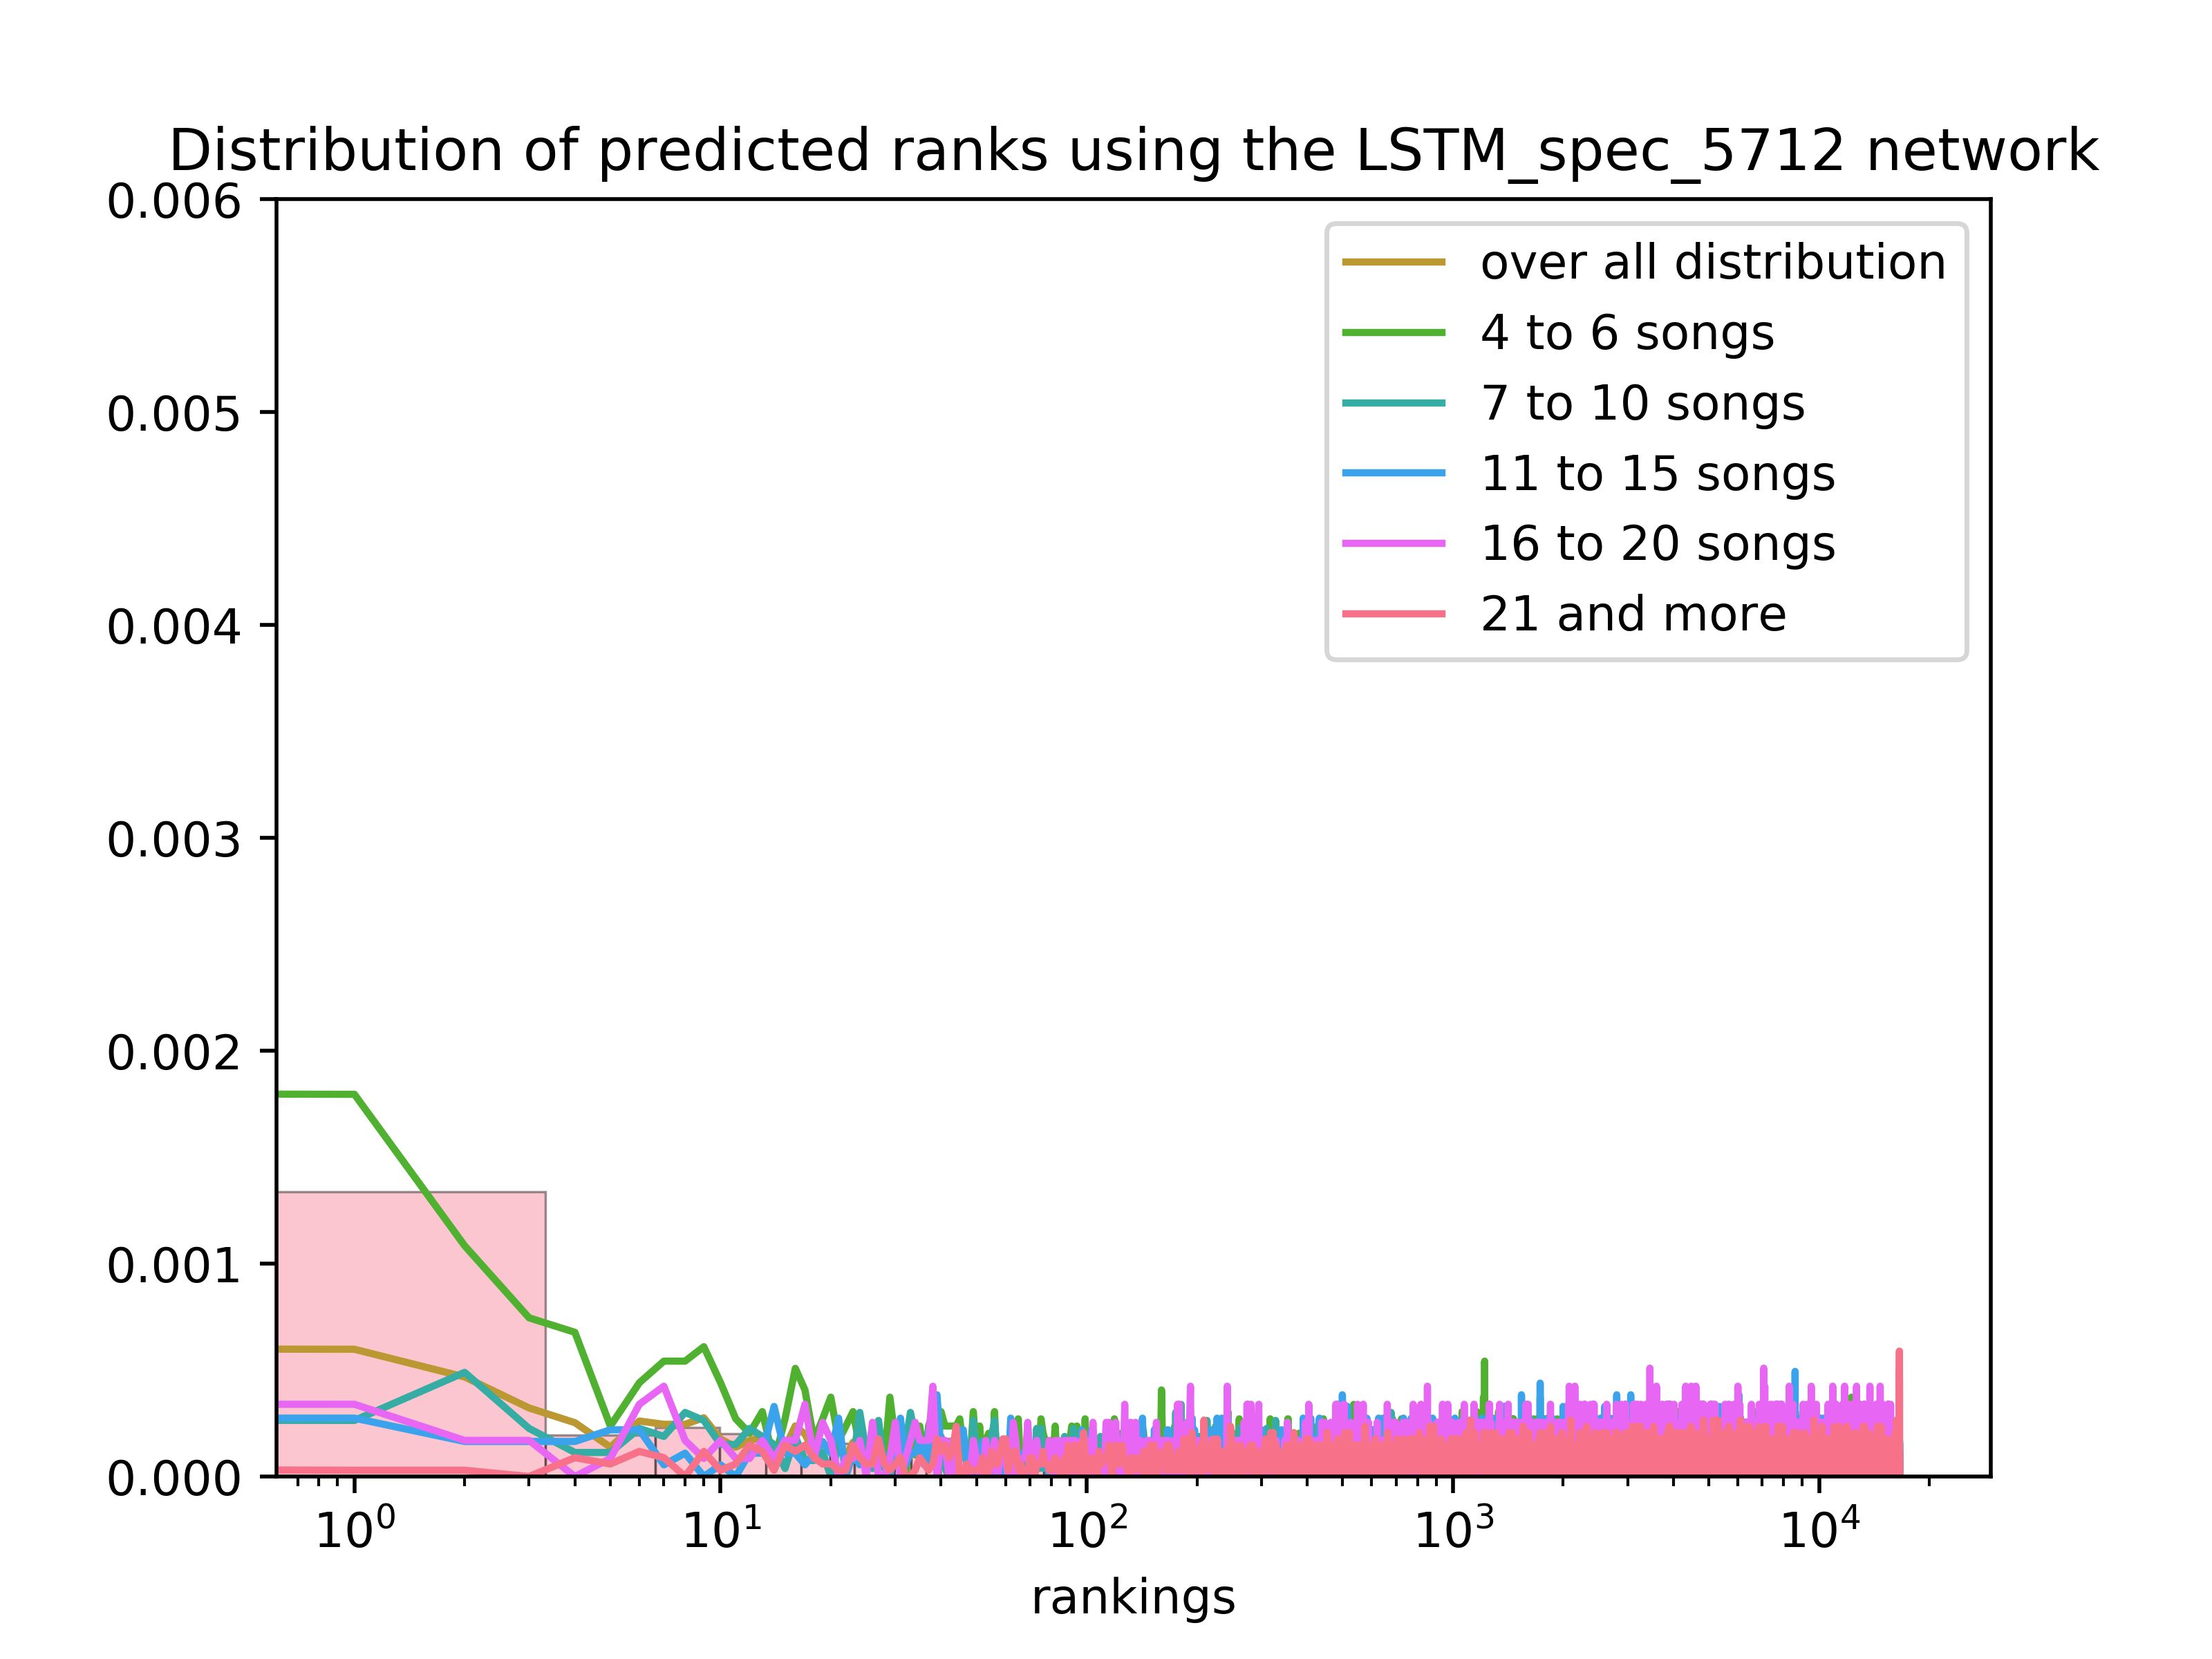
\includegraphics[width=1\linewidth]{./img/lstm_spec_5712_graph.png}
  \caption[RDG of the LSTM\_spec\_5712 method]{RDG of the \newline LSTM\_spec\_5712 method}
  \label{fig:lstm_spec_5712_distribution}
\end{minipage}
\end{figure}\label{fig:lstm_spec_distributions}

\subsection{GRU and LSTM networks with Mel-spectrogram input}\label{ssec:GRU_LSTM_mel_results}

Methods with mel-spectrograms as input seem to yield better results than methods with spectrogram inputs and GRU\_mel network confirms it as it has the best results within the neural network method group. The GRU\_mel network performed better than the one with LSTM layers and also showed the smallest training loss. Figures \ref{fig:gru_mel_distribution} and \ref{fig:lstm_mel_distribution} display typical tendencies most of the methods have, with the sharp drop for short playlists and more stability for longer playlists. This is more apparent with the GRU\_mel method. For the LSTM\_mel, longer playlists drop unconventionally early. 

Table \ref{table:mel_spec_methods} puts recalls and nDGC of "mel" neural networks into perspective with other "mel" methods.
As we can see, the GRU\_mel network placed 4.6\% of songs into the top 10, 5.7\% into the top 50 and 6.3\% into the top 100. The LSTM\_mel network is worse. It puts 3.2\% of songs in the top 10. For \textit{R@50} and \textit{R@100} it outperforms raw mel-spectrograms with 4.3\% of songs in the top 50 and 5\% of songs with assigned ranks in the top 100.

\begin{figure}[h]
\centering
\begin{minipage}{.45\textwidth}
  \centering
  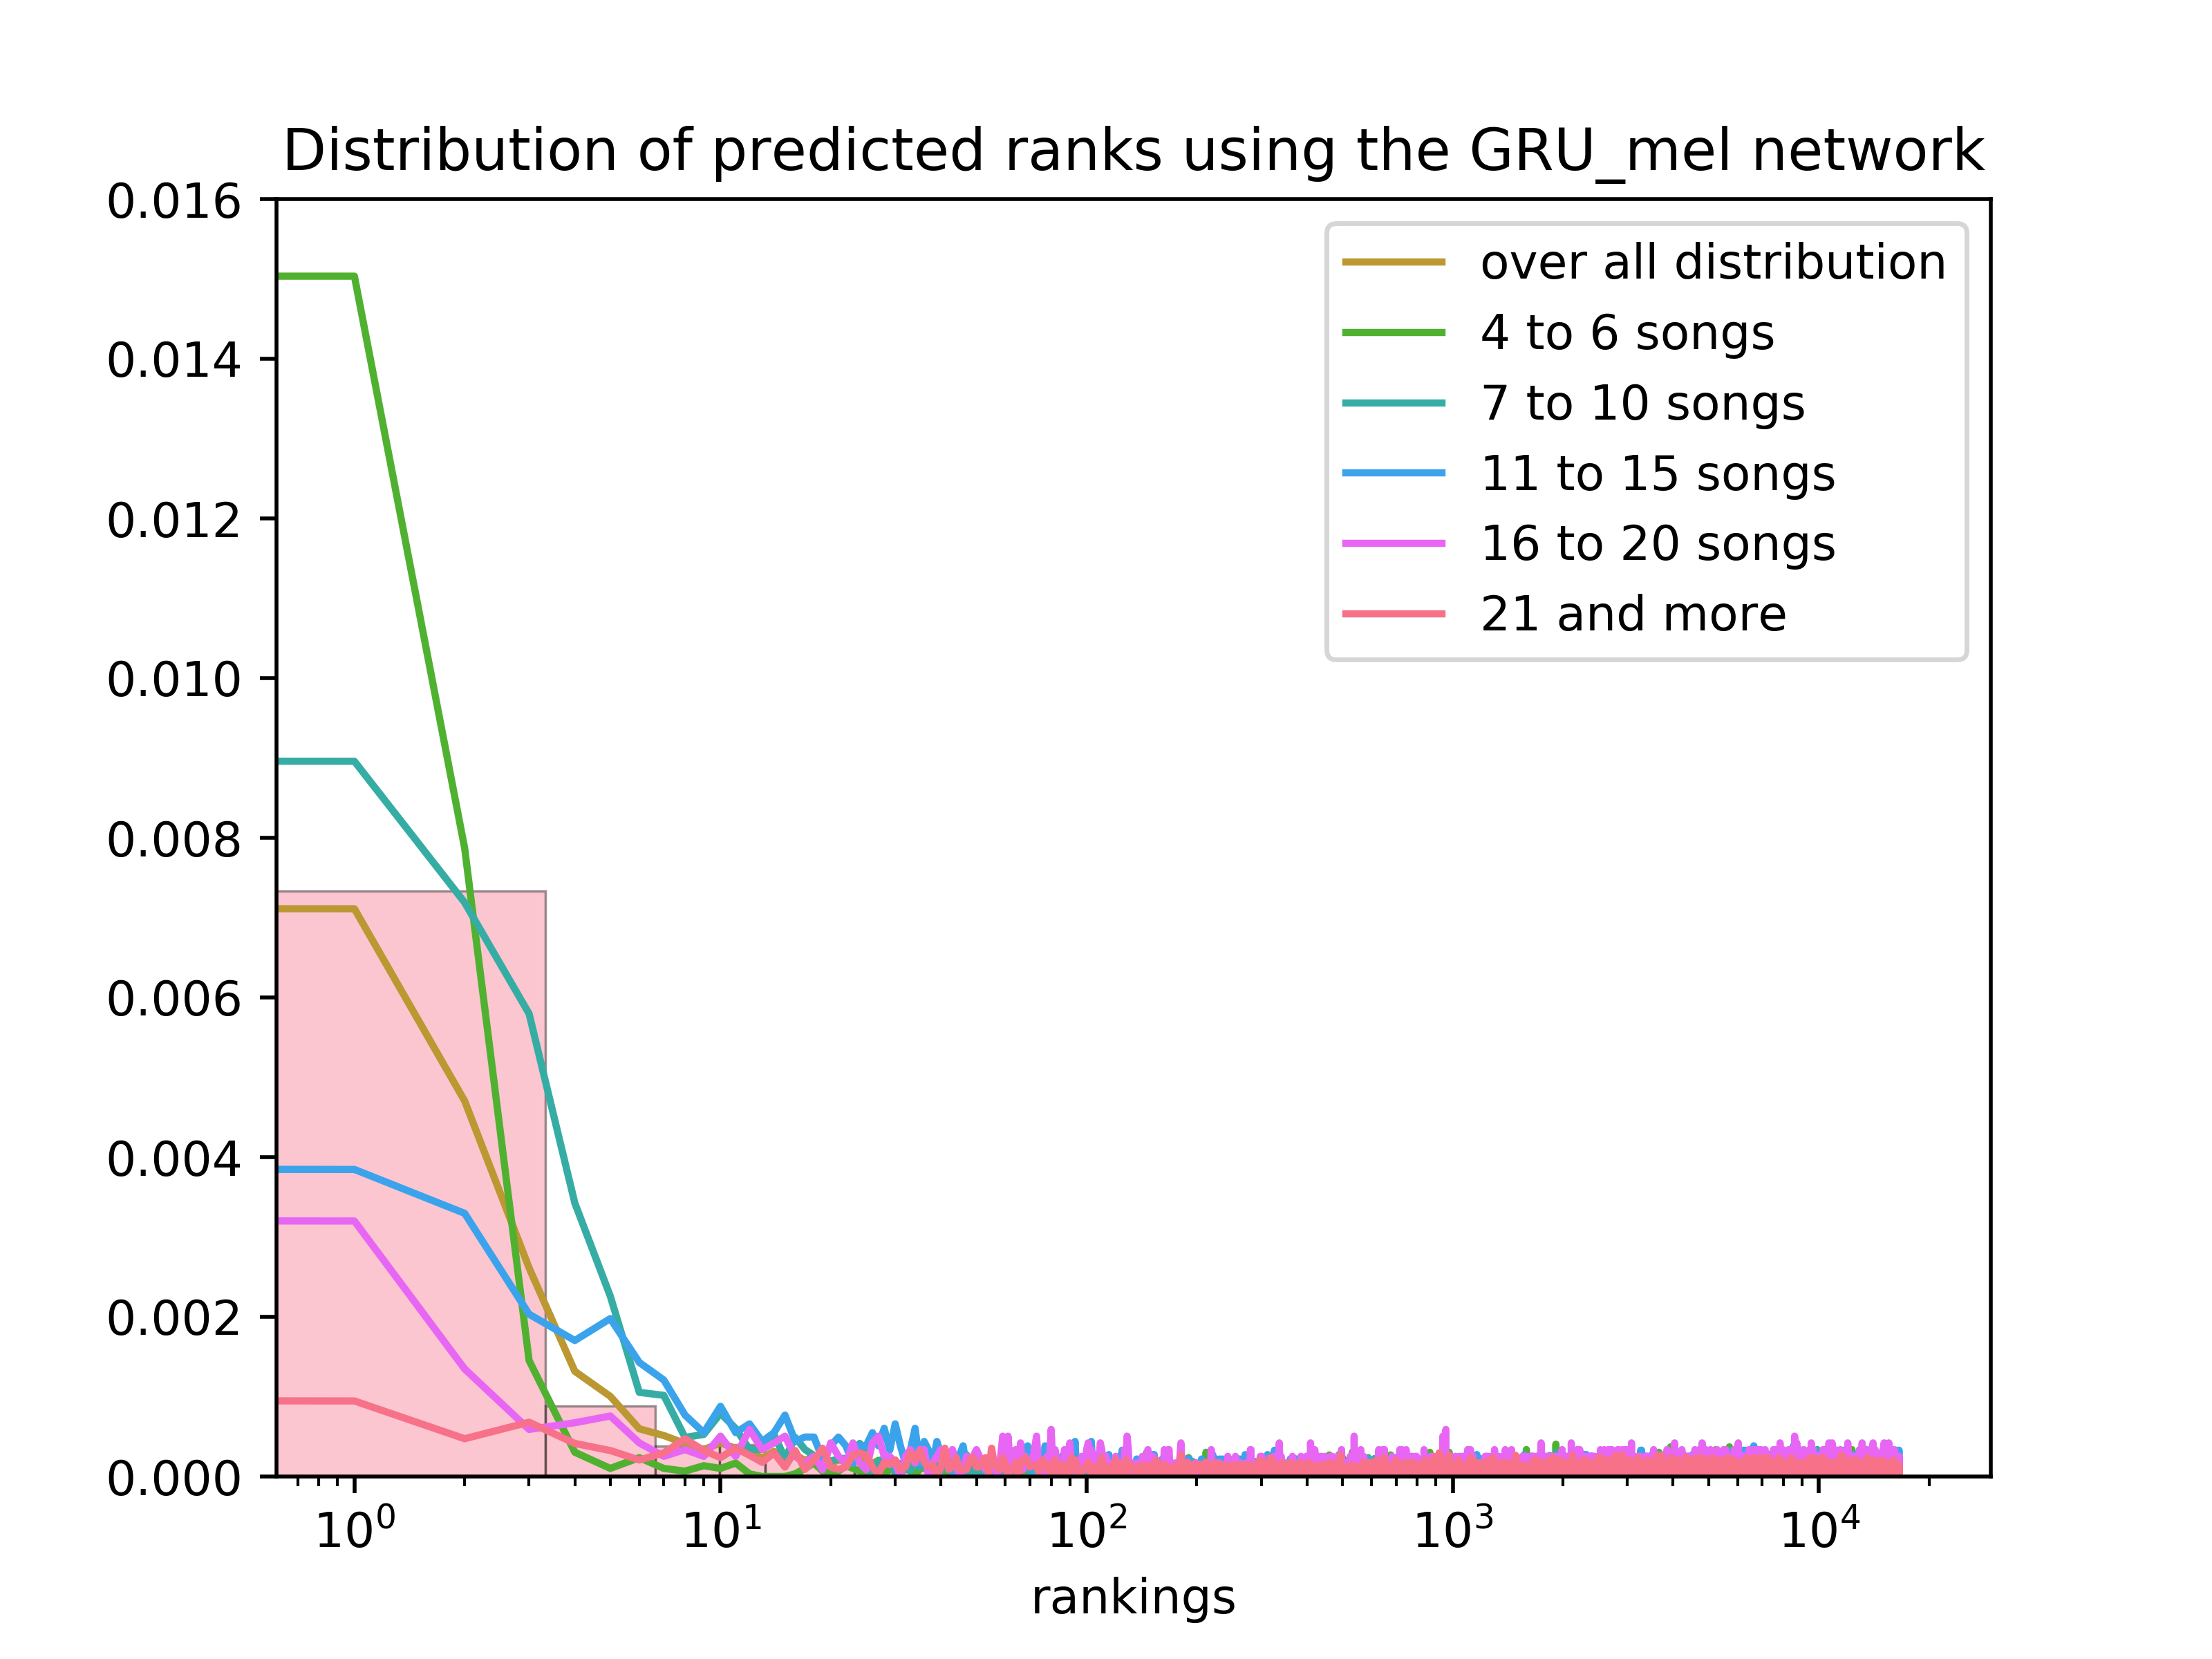
\includegraphics[width=1\linewidth]{./img/gru_mel_graph.png}
  \caption[RDG of the GRU\_mel method]{RDG of the \newline GRU\_mel method}
  \label{fig:gru_mel_distribution}
\end{minipage}
 \vspace{1cm}
\begin{minipage}{.45\textwidth}
  \centering
  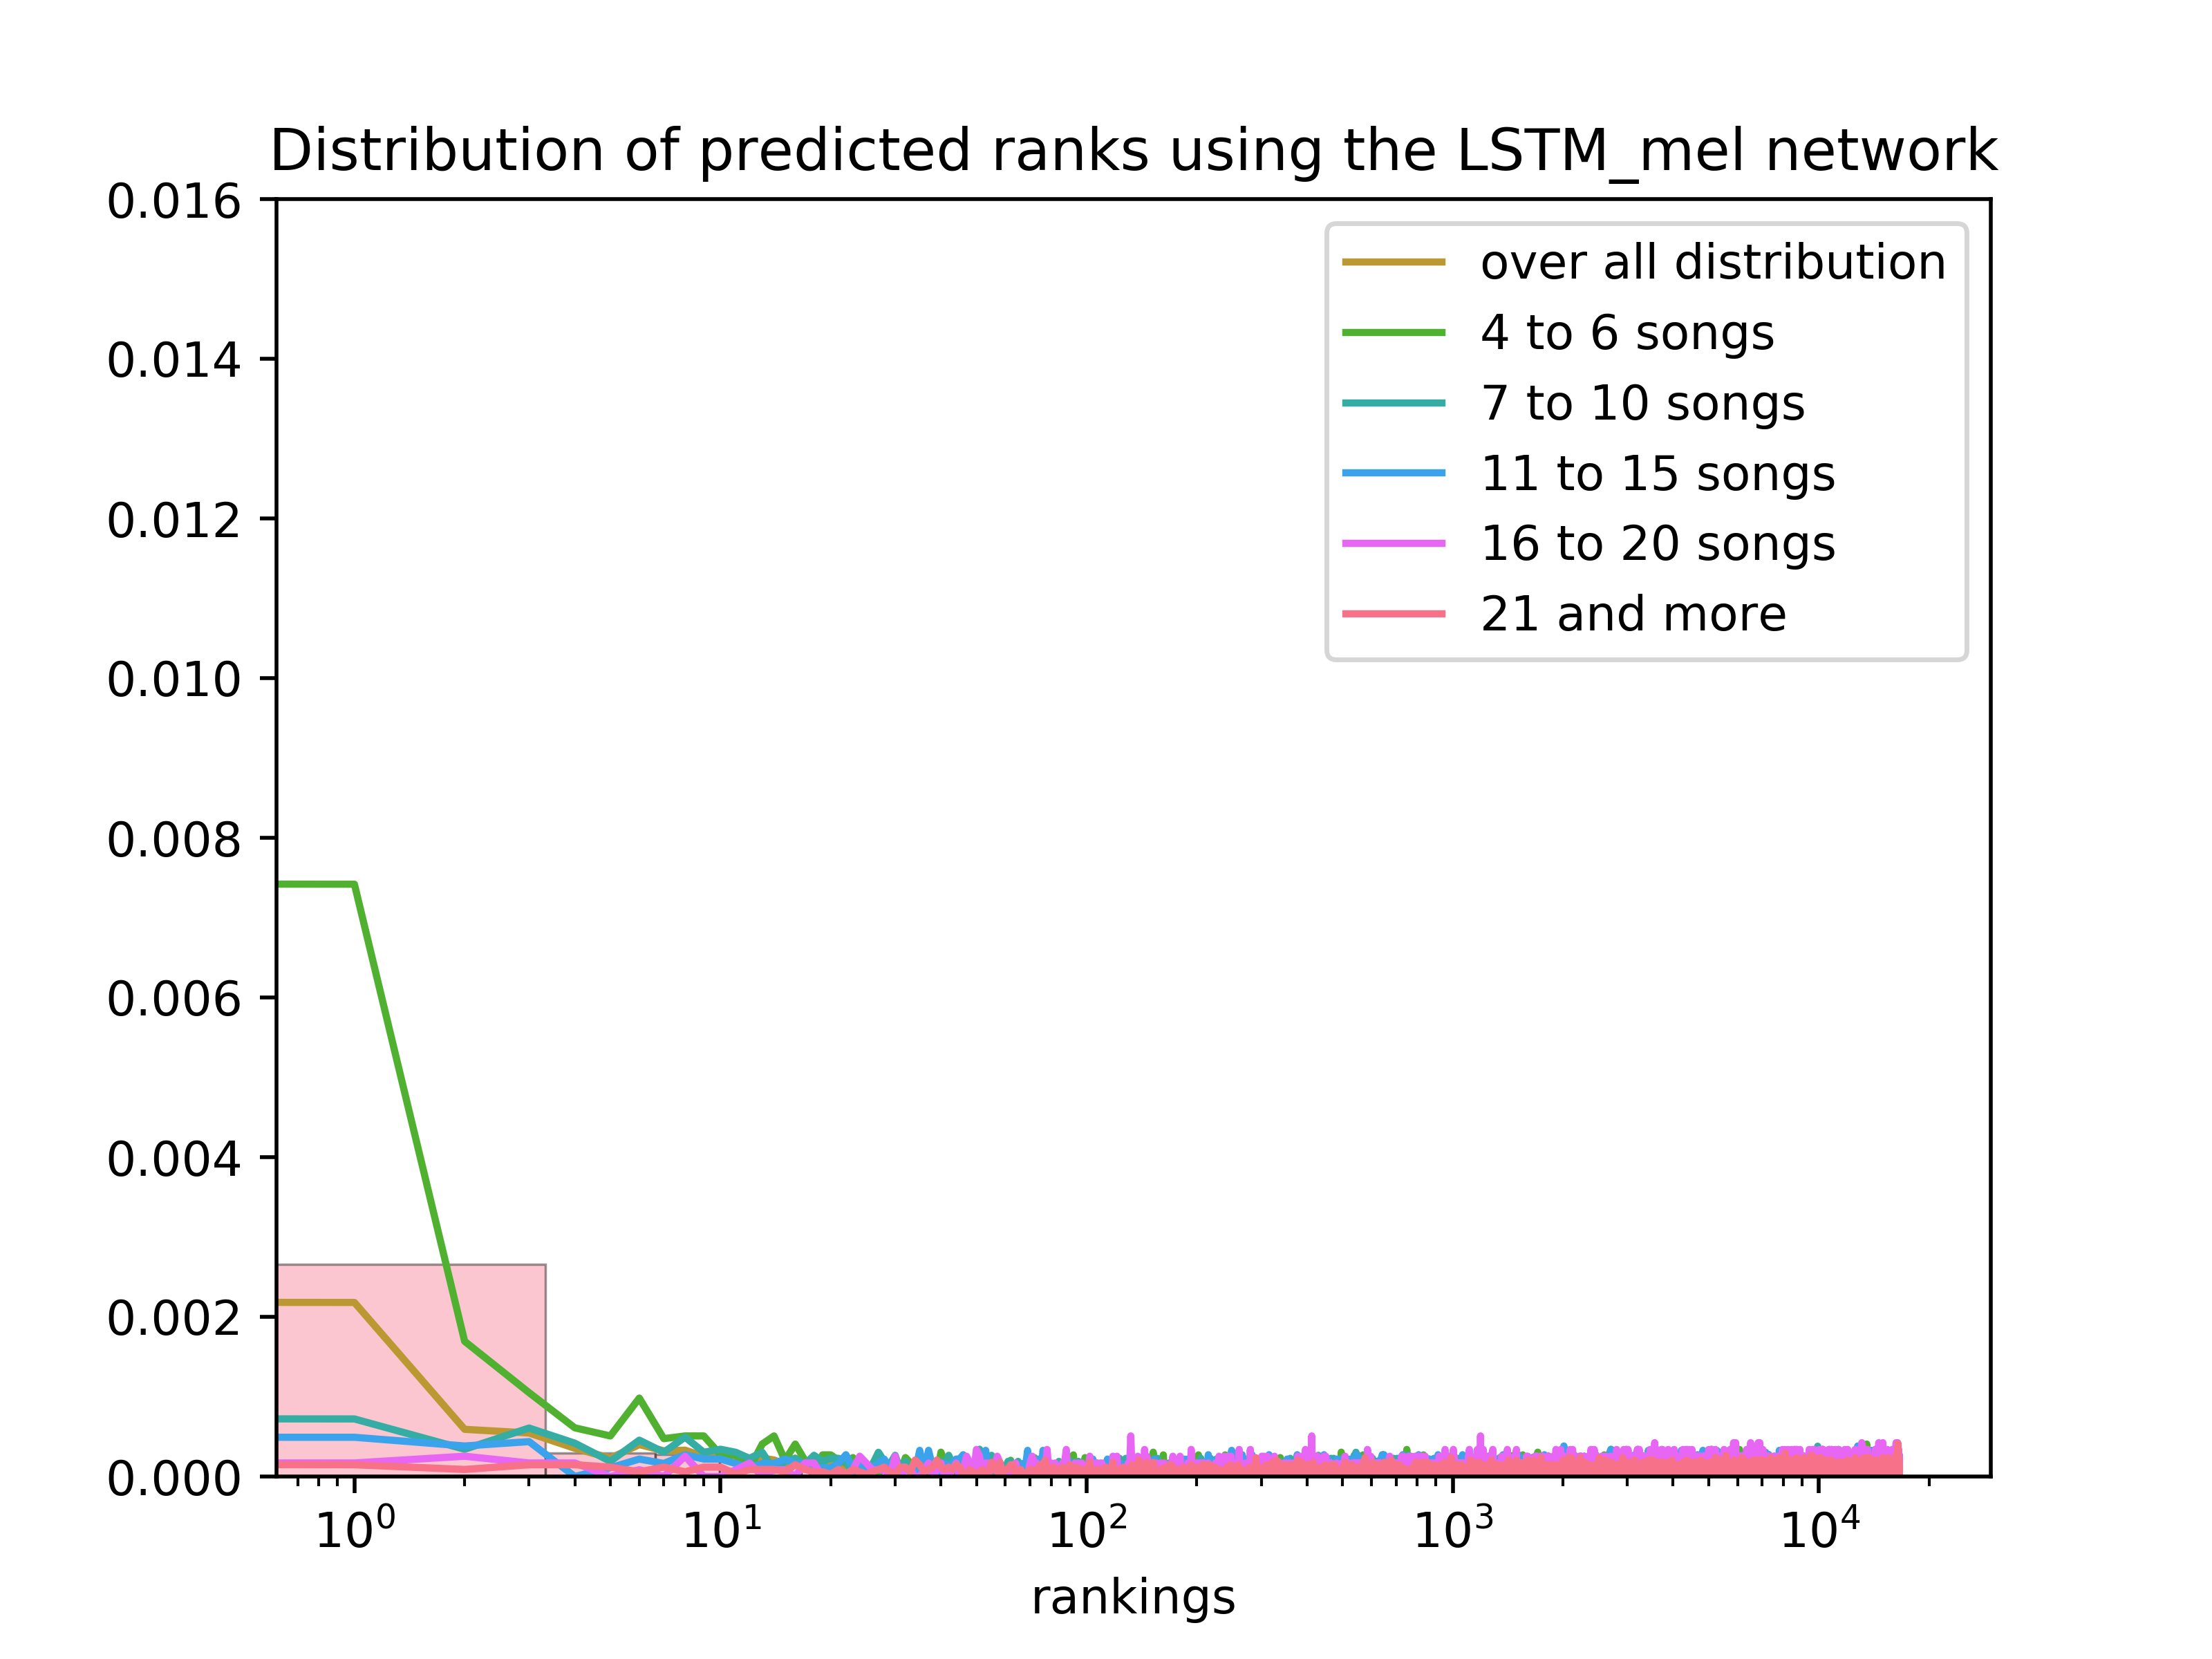
\includegraphics[width=1\linewidth]{./img/lstm_mel_graph.png}
  \caption[RDG of the LSTM\_mel method]{RDG of the \newline LSTM\_mel method}
  \label{fig:lstm_mel_distribution}
\end{minipage}
\end{figure}\label{fig:mel_nn_distributions}

\subsection{GRU and LSTM networks with MFCC input}\label{ssec:GRU_LSTM_MFCC_results}
The MFCC networks seem to have the biggest potential of improving if they were to be trained for a longer period of time as their losses in Figure \ref{fig:all_model_training} do not stagnate as much towards the end of training as the other networks. This is especially true for the GRU\_MFCC network. They would, however, probably never achieve a loss as small as the "mel" networks have. 

Compared to the raw MFCCs the GRU\_MFCC and LSTM\_MFCC were an improvement as the values in Table \ref{table:mfcc_methods} suggest. The Figures \ref{fig:gru_mfcc_distribution} and \ref{fig:lstm_mfcc_distribution} containing both method's \textit{RDGs} indicate the superiority of the LSTM\_MFCC method over the GRU\_MFCC. Both methods made a huge jump upwards with the threshold similarity. Without it, they were at the bottom of the tested methods as the orange color suggests in Figure \ref{fig:no_threshold_method_comparison}, but the threshold helped them to perform around average as they are in the green-yellow zone in Figure \ref{fig:threshold_method_comparison}.

\begin{figure}[H]
\centering
\begin{minipage}{.45\textwidth}
  \centering
  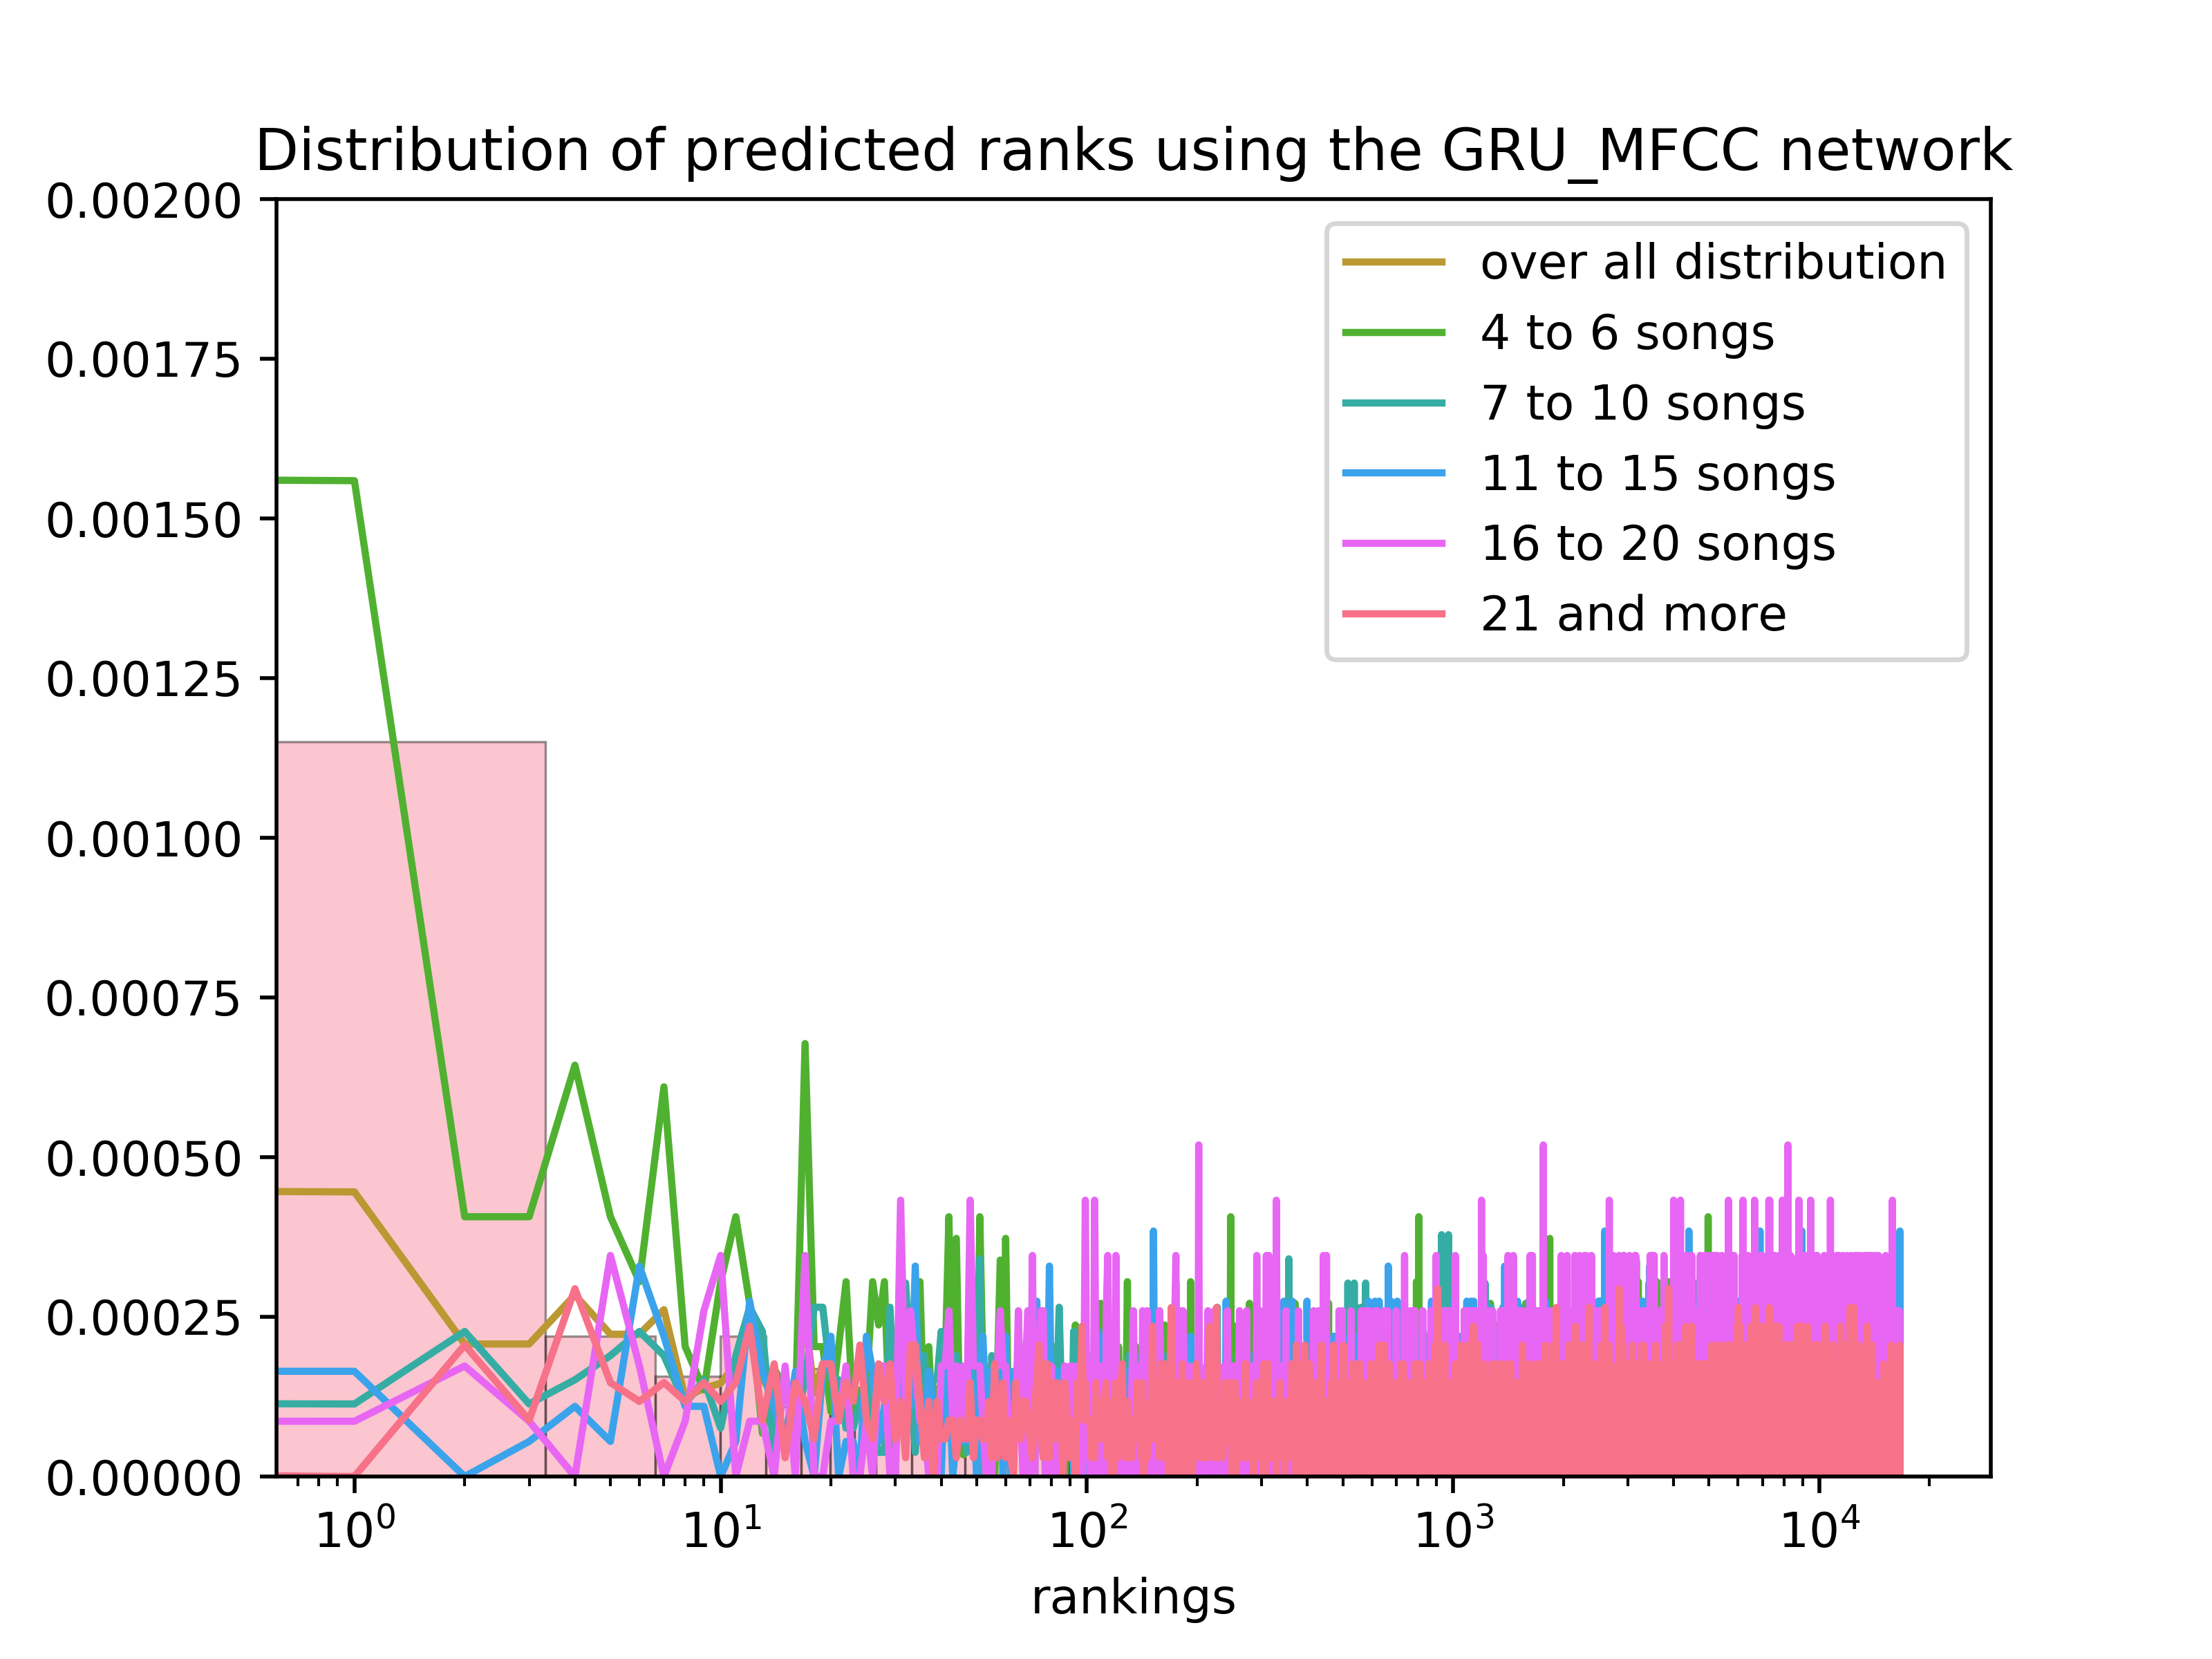
\includegraphics[width=1\linewidth]{./img/gru_mfcc_graph.png}
  \caption[RDG of the GRU\_MFCC method]{RDG of the \newline GRU\_MFCC method}
  \label{fig:gru_mfcc_distribution}
\end{minipage}
 \vspace{1cm}
\begin{minipage}{.45\textwidth}
  \centering
  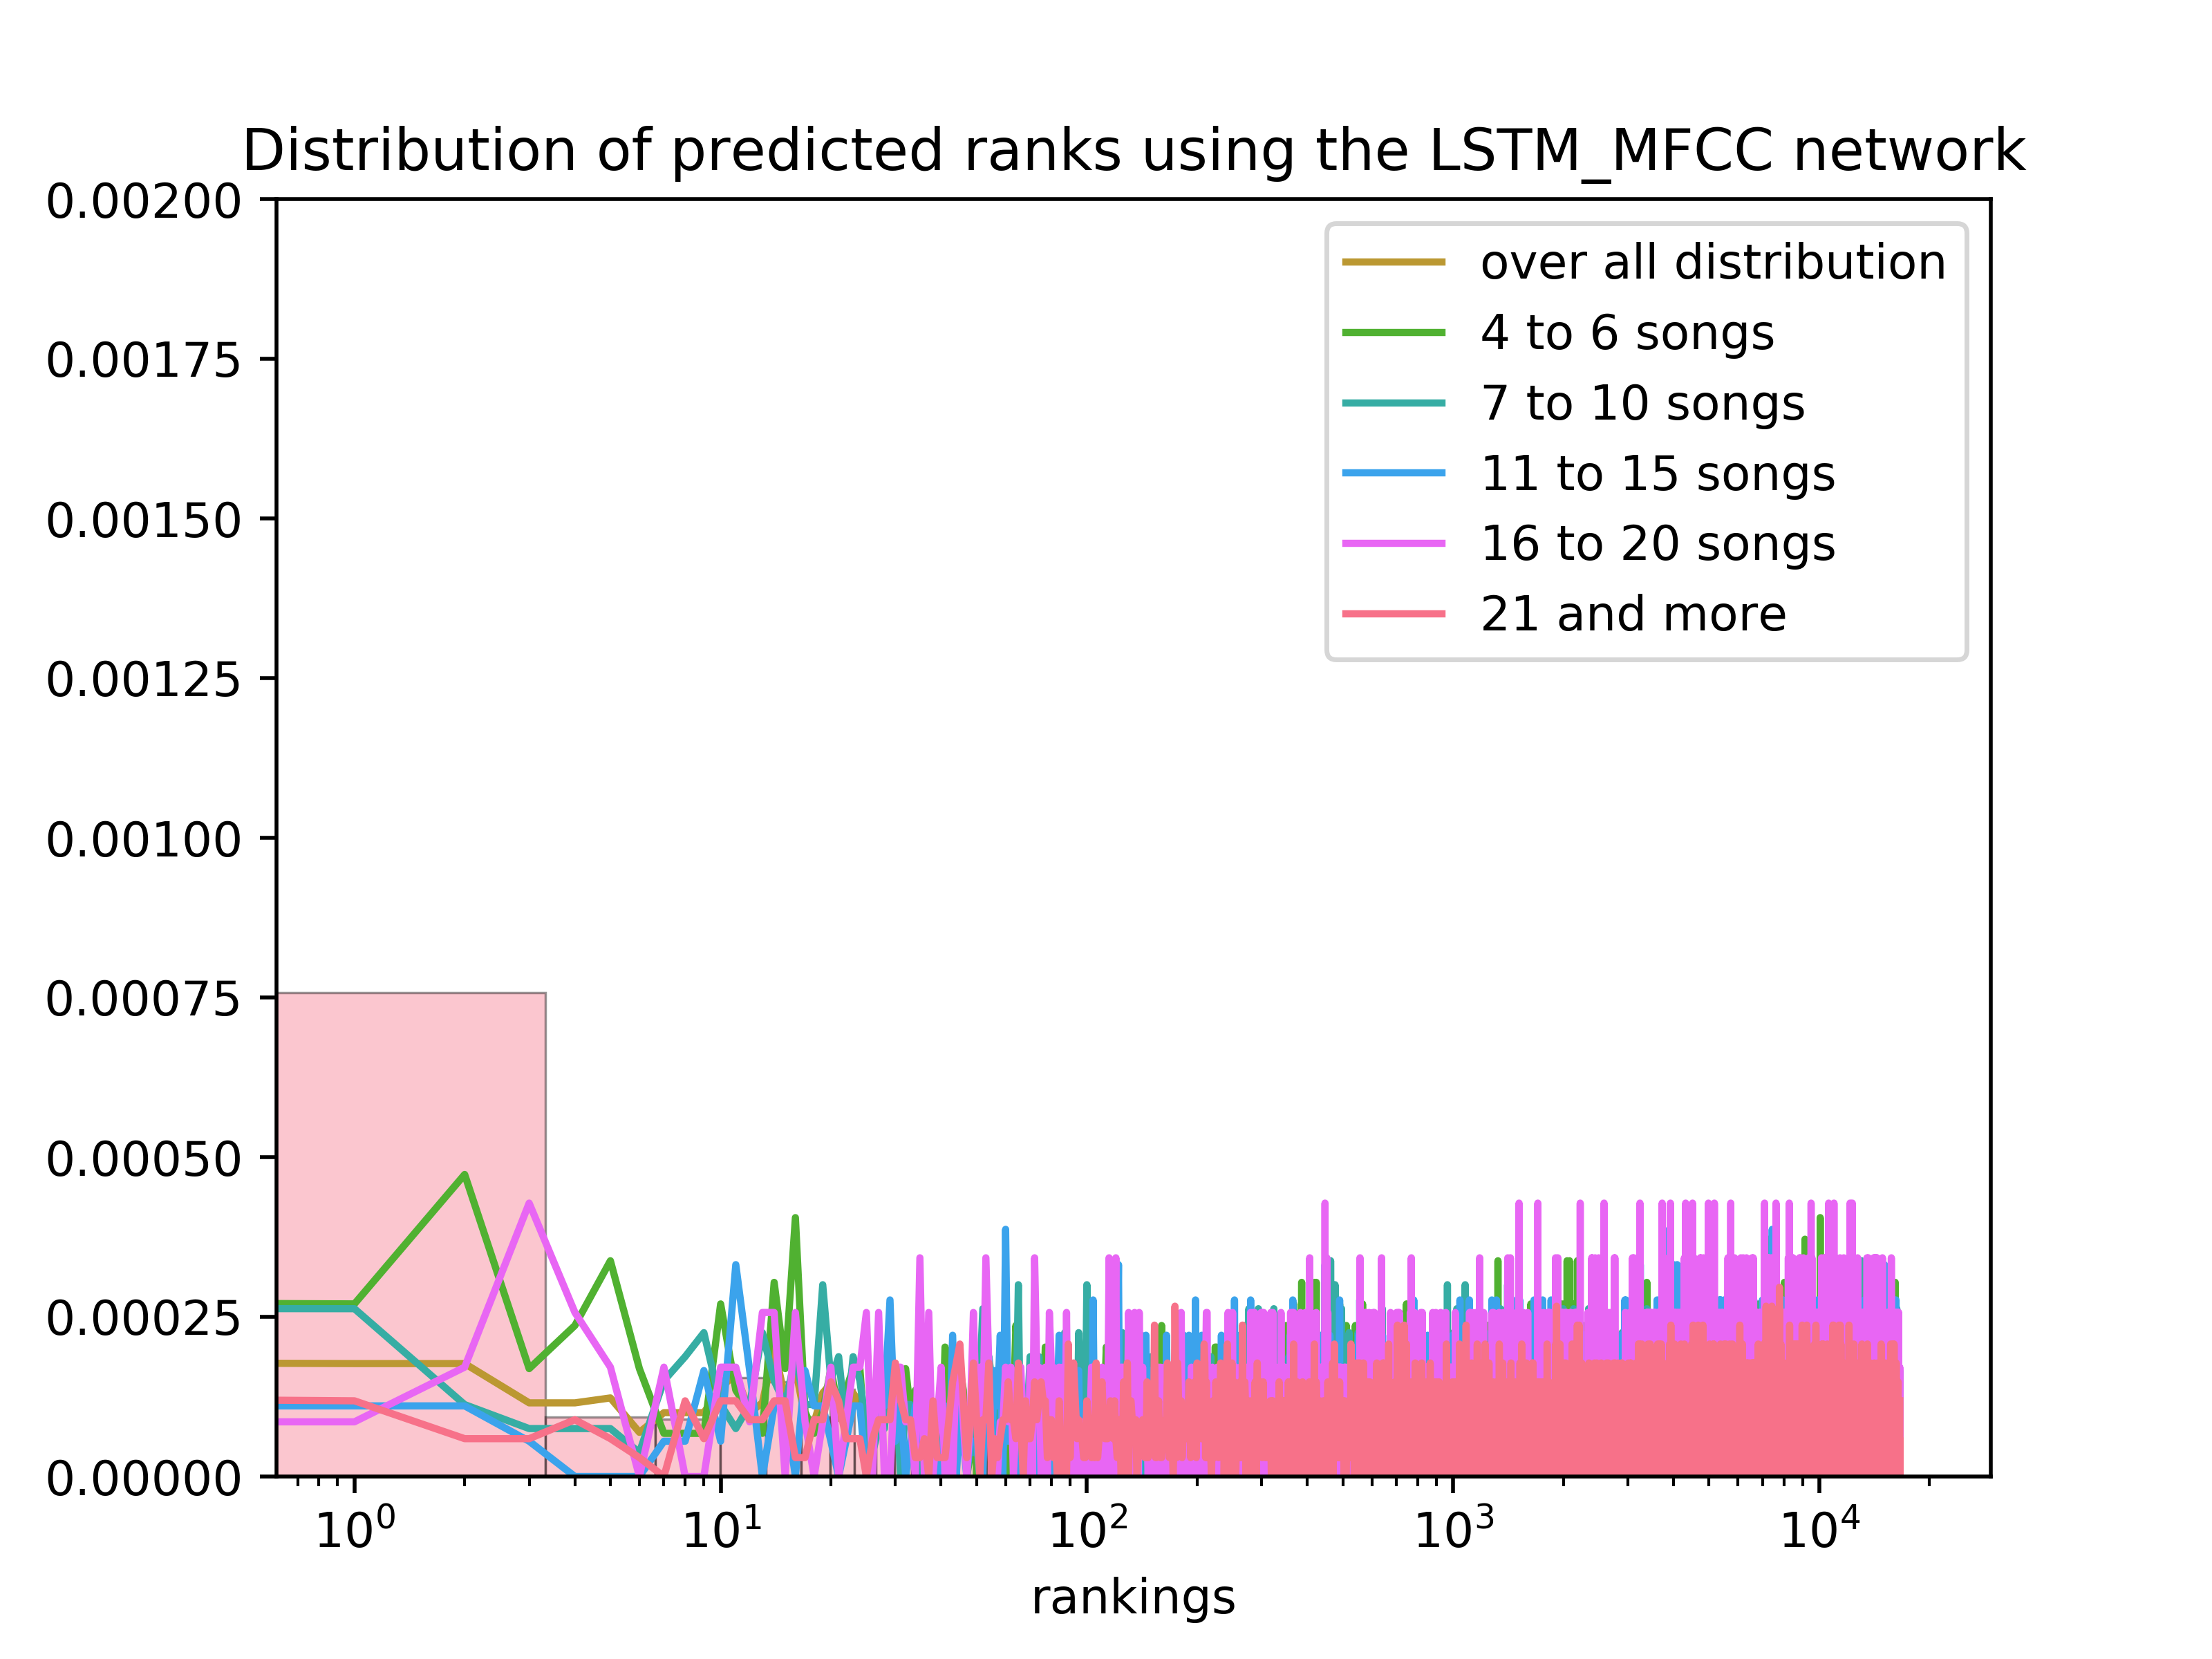
\includegraphics[width=1\linewidth]{./img/lstm_mfcc_graph.png}
  \caption[RDG of the LSMT\_MFCC method]{RDG of the \newline LSMT\_MFCC method}
  \label{fig:lstm_mfcc_distribution}
\end{minipage}
\end{figure}\label{fig:mfcc_nn_distributions}

\section{Discussion}\label{sec:discussion}
In this section we first state, in Subsection \ref{ssec:exp_vs_reality}, 
if the results match the expectations from Section \ref{sec:expectations}. Then to summarize the results and put all the 
methods into perspective we did two things. First in Subsection 
\ref{ssec:relative_comparison} we compared the methods relatively to each 
other. Secondly in Subsection \ref{ssec:absolute_results} we focused on the 
values of the evaluation measures compared to values of random recommendations and we also considered what the absolute numbers of the evaluation measures suggest. This was to estimate the recommendation qualities of our methods. In subsection \ref{ssec:additional findings} we introduce multiple graphs of performance depending on properties which we found during the evaluation could correlate with it. 

\subsection{Expectations vs. reality}\label{ssec:exp_vs_reality}
Let's recapitulate what we expected. First we expected, that audio-based methods will perform better than lyrics-based methods. Because the best
method -- PCA\_Tf-idf -- is a lyrics based method, we cannot say that this 
prediction was confirmed. Raw Tf-idf also performed very well compared to 
others and outperformed most audio-based methods.  The W2V was a little 
behind and the SOM network was a failure, however we definitely cannot declare,
that when a method is audio-based it means it will have better results than a lyrics-based method.

There are various theories that could explain this. It could be connected to the user dataset we did the evaluations on. Therefore, we tested the playlists on 
diversity. To calculate diversity of a playlist, we divided the number of unique artists it contained with its length. When we averaged over all the playlists of length at least four, we got 0.83 which means, that an 
artist rarely repeats in a playlist. 

This variety could have suited the 
Tf-idf and PCA\_Tf-idf methods as the presumed diversity of their recommendations poses 
an advantage for such heterogeneous playlists. To test this hypothesis, we 
took 1000 random songs and found 100 most similar songs for each of the songs using each of the tested methods. We than computed the average diversity of the 101 song playlists for each method as we did for the playlists in the dataset. The results are in Table \ref{table:diversity_table}.

\begin{table}[h]
\centering

%\renewcommand{\arraystretch}{1.5}
\begin{tabu} to 1.7\textwidth {| c | c |}
\hline
\textbf{method} & \textbf{playlist diversity} \\
\hline
PCA\_mel\_5715 & 0.739 \\
\hline
PCA\_mel\_320 & 0.746 \\
\hline
PCA\_spec\_1106 & 0.700 \\
\hline
PCA\_spec\_320 & 0.702 \\
\hline
LSTM\_mel & 0.749 \\
\hline
GRU\_mel & 0.725 \\
\hline
LSTM\_spec\_20400 & 0.721 \\
\hline
GRU\_spec\_20400 &  0.752\\
\hline
LSTM\_spec\_5712 & 0.729 \\
\hline
GRU\_spec\_5712 &  0.751 \\
\hline
LSTM\_mfcc & 0.794 \\
\hline
GRU\_mfcc & 0.776 \\
\hline
TF-idf & 0.800 \\
\hline
SOM\_W2V & 0.861 \\
\hline
PCA\_tf\_idf & 0.812 \\
\hline
W2V & 0.71186 \\
\hline
\end{tabu} 
\caption{Table containing the value of the diversity index that was also calculated for the UD we have.}
\label{table:diversity_table}
\end{table}
As one can see, the most diverse method is SOM\_W2V which is not very surprising as it yields basically random results. Nonetheless, the best lyrics methods, PCA\_Tf-idf and Tf-idf are those wiinzh the second and third biggest diversity which confirms, that is probably where lays their advantage.

Another reason for the evenness of the audio and lyrics-based methods might be, that 15 seconds from each song's audio was not enough and if we made the excerpts longer, the results for audio-based methods would have been better. \\

We also expected that more advanced methods will outperform simpler methods. This did not happen at all. The Tf-idf which we though of as a simple baseline outperformed almost all of the other methods. Overall, PCA methods were the most successful ones (with the exception of PCA\_spec\_320) and left the neural networks behind. 

This could be caused by the fact that we did not tune our neural networks. There is not much to improve about the PCA but a lot of parameter optimisation and also architecture re-creation can be done on all of the neural networks we implemented. Moreover, the training conditions can be also altered. The batch size as well as the number of epochs can be lowered or increased. 

\subsection{Relative results}\label{ssec:relative_comparison}

We created two heat maps to compare the methods mutually. One is depicted in Figure \ref{fig:no_threshold_method_comparison} for results without threshold and one in Figure \ref{fig:threshold_method_comparison} for results with threshold. We ranked the methods on how well they performed in each evaluation measure and we took playlist lengths into account. 

We can see, that the PCA\_Tf-idf was the most successful method winning in 8 out of the 20 measures. It performed best on long playlists. The average rank, where its performance is in the red area, is not that important for recommendation. We included it to have some understanding of what is going on on throughout the ranks, not only at the first 100 places which are most important for recommendation.

Second comes PCA\_mel\_5715, then Tf-idf with PCA\_spec\_1106 right behind it. Then we have the GRU\_mel method which is orange for short playlists, however otherwise in the green area and it is the best neural network method, lyrics or audio-based. 

Overall we can see, that the PCA methods were very successful compared to other methods. Except of the PCA\_spec\_320, they are all green and the only method that comes between them on the top places 4 is the Tf-idf. 

Within text-based methods, the PCA\_Tf-idf and Tf-idf show strong dominance, the W2V is below average and the SOM has the worst results of all methods. For audio-based methods, the winner is PCA\_mel\_5715. \\

\begin{figure}[h]
    \centering
	\includegraphics[width=1\linewidth]{./img/no_threshold_method_ranking.png}
	\caption[Method performance comparison heat map without threshold applied]{Method performance comparison heat map without threshold applied. \\ The relative performance of methods based on how they performed for various evaluation measures when similarity was defined without threshold. Each method was assigned a rank from 1 to 16 (16 is the number of the methods in this figure) for each measure based on how it performed for the particular measure compared to the other methods. The more darker green the better was the performance, yellow are the average ones and red are the for the worst performances. The evaluation measures are displayed on the x-axis. Measures with "\_L" appended contain results of long playlists (length 16 and longer), measures with "\_M" are the results for medium playlists (length 8-15) and measures with "\_S" are evaluation measures of short playlists (length 4-7). When there is nothing appended to the evaluation measure name, it is the value for all playlists.}
	\label{fig:no_threshold_method_comparison}
\end{figure}
\begin{figure}[h]
    \centering
	\includegraphics[width=1\linewidth]{./img/threshold_method_ranking.png}
	\caption[Method performance comparison heat map with threshold applied]{Method performance comparison heat map with threshold. \\ The relative performance of methods based on how they performed for various evaluation measures when similarity was defined with threshold. Each method was assigned a rank from 1 to 16 (16 is the number of the methods in this figure) for each measure based on how it performed for the particular measure compared to the other methods. The more darker green the better was the performance, yellow are the average ones and red are the for the worst performances. The evaluation measures are displayed on the x-axis. Measures with "\_L" appended contain results of long playlists (length 16 and more), measures with "\_M" are the results for medium playlists (length 8-15) and measures with "\_S" are evaluation measures of short playlists (length 4-7). When there is nothing appended to the evaluation measure name, it is the value for all playlists.}
	\label{fig:threshold_method_comparison}
\end{figure}

\subsection{Absolute results}\label{ssec:absolute_results}
Because we did not perform classification on a standardised set and no one has used the datasets we are using to evaluate their algorithms, it is a little challenging to find something outside of this thesis what we could compare the results to.

We decided to compare our methods to random suggestions. If songs were assigned ranks from 1 to 16,594 in a uniform distribution, meaning each rank had the probability of $1/16594$ to be assigned to a song the values of the recall evaluation measures would be following:
\begin{itemize}
    \item R@10 =  $ 10*(1/16594) $ = 0.06\% of songs
    \item R@50 = $ 50*(1/16594) $ = 0.3\% of songs
    \item R@100 = $ 100*(1/16594) $ = 0.6\% of songs
\end{itemize}

Knowing this, we created Figure \ref{fig:absolute_evaluation_comparison} showing the multiples of how many times a method is better than random recommendation would be. We divided it into categories based on playlist length. Measures with \_L" appended contain results of long playlists (length 16 and more), methods with "\_M" are the results for medium playlists (length 8-15) and methods with "\_S" are evaluation measures of short playlists (length 4-7). When there is nothing appended to the evaluation measure name, it is the value for all playlists. We can see, that there is major improvement especially for values of R@10 where the best method, the PCA\_Tf-idf is 90.3 times better than random recommendation. This means, that when random recommendation places 0.06\% of songs into the top 10, the PCA\_Tf-idf places $90.3*0.06\%$ of songs into the top 10. 

If we disregard the SOM\_W2V and GRU\_spec\_5712 methods which appear to be basically random, we can see, that the rest of the methods are significantly better than random suggestions. Especially for the first ten ranks, it seems that with the method we implemented, we can provide relevant recommendations. \\

However, if we look at it from another perspective and realize that if using the best method --- PCA\_Tf-idf we placed 6.6\% of songs into the top 100, and 93.4\% percent of songs somewhere further, we probably want a recommendation system to perform better. Nevertheless, some of the methods have shown great potential of providing good recommendations and with for example more parameter optimisation for the neural networks they could improve even more. An incorporation into a collaborative-filtering recommender system, could also be a good idea.

\begin{figure}[h]
    \centering
	\includegraphics[width=1\linewidth]{./img/absolute_evaluation_comparison.png}
	\caption[Method comparison to random suggestions heat map]{Method comparison to random suggestions heat map. \\
Each rectangle contains the multiple of how many times the method on its corresponding y coordinate is better than random suggestions of the evaluation measure on the corresponding x coordinate. For example if random recommendation would place 0.5\% of songs into the top 10 meaning, that its value for R@10 was 0.005 the Tf-idf method would place $84.1*0.05\%$ of songs into the top ten so the value of R@10 for Tf-idf would be $84.1*0.005$ because 84.1 is the value in the rectangle that has Tf-idf on the y coordinate and R@10 at the x coordinate.}
	\label{fig:absolute_evaluation_comparison}
\end{figure}

\subsection{Additional findings}\label{ssec:additional findings}
Additionally we also created some interesting graphs. We tried to find a correlation between the training loss of neural networks and their recommendation performance. The training curves are displayed in Figure \ref{fig:all_model_training}. 

Figure \ref{fig:training_correlation_graph} visualizes the dependency of the values the evaluation measure of neural networks (y-axis) on the training loss the neural networks had when finished training (x-axis). We can see, that except of the four dots in the upper right corner that belong to the GRU\_spec\_20400 method, there is some correlation that suggests that a smaller training loss indicates better recommendations. This would be logical as 

\begin{figure}[h]
    \centering
	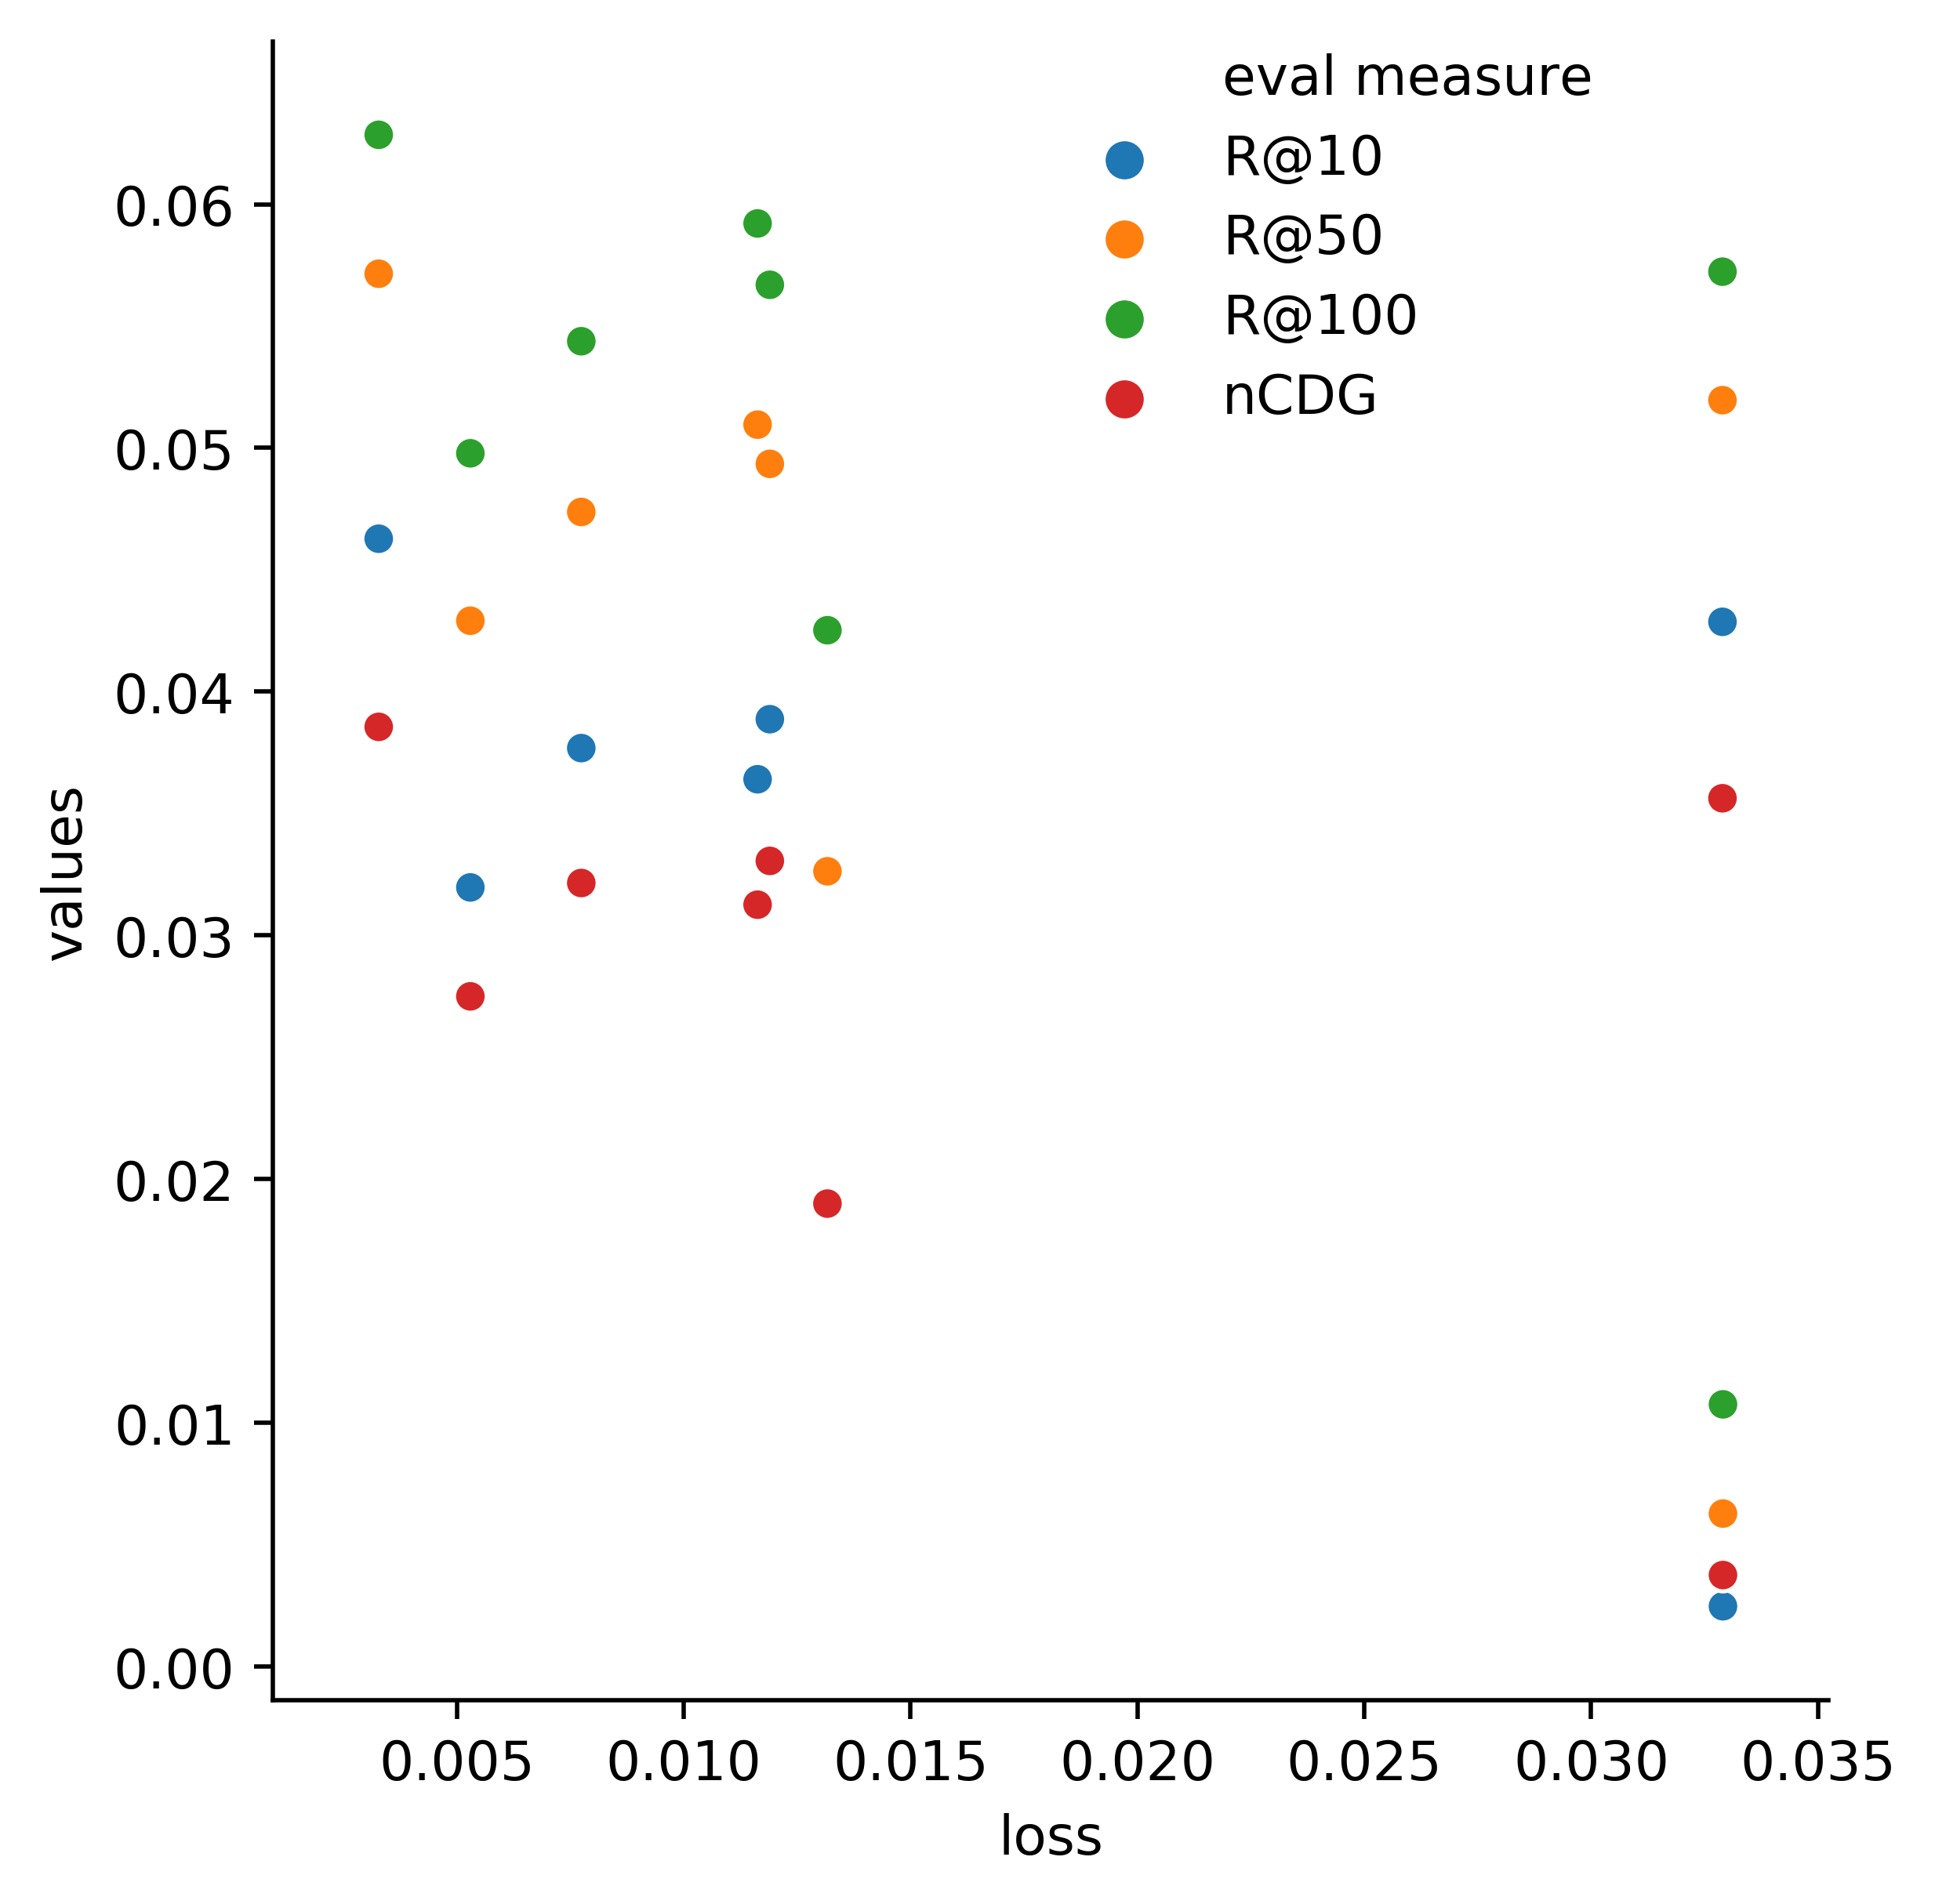
\includegraphics[width=1\linewidth]{./img/nn_training_performance_correlation.png}
	\caption[Training loss and performance correlation graph]{Training loss and performance correlation graph. \\ This graph visualized the correlation between the final training loss displayed on the x axis and the performance of neural networks on various evaluation measures. The values of the evaluation measures are displayed on the y axis. Each evaluation measure has a different color which is illustrated in the legend.}
	\label{fig:training_correlation_graph}
\end{figure}

The 0.03\%-threshold inspired us to look at the relative similarities between songs for each method because the value of the threshold varied a lot for different methods. We again created a correlation graph between the performance of methods and the value of the 0.03\%threshold. It is depicted in Figure \ref{fig:threshold_correlation_graph}. We can see, that for methods with threshold values smaller than 0.5 there is a visible trend of better performance being dependant on smaller threshold value. Then there is a big gap as no method had its threshold value between 0.5 and 0.95. For the methods with threshold close to 1 correlation is not present. Some are very low which would follow the trend of thresholds between 0 and 0.5 but there is a significant number of methods that have good results and do not follow the decrease in performance.

\begin{figure}[h]
    \centering
	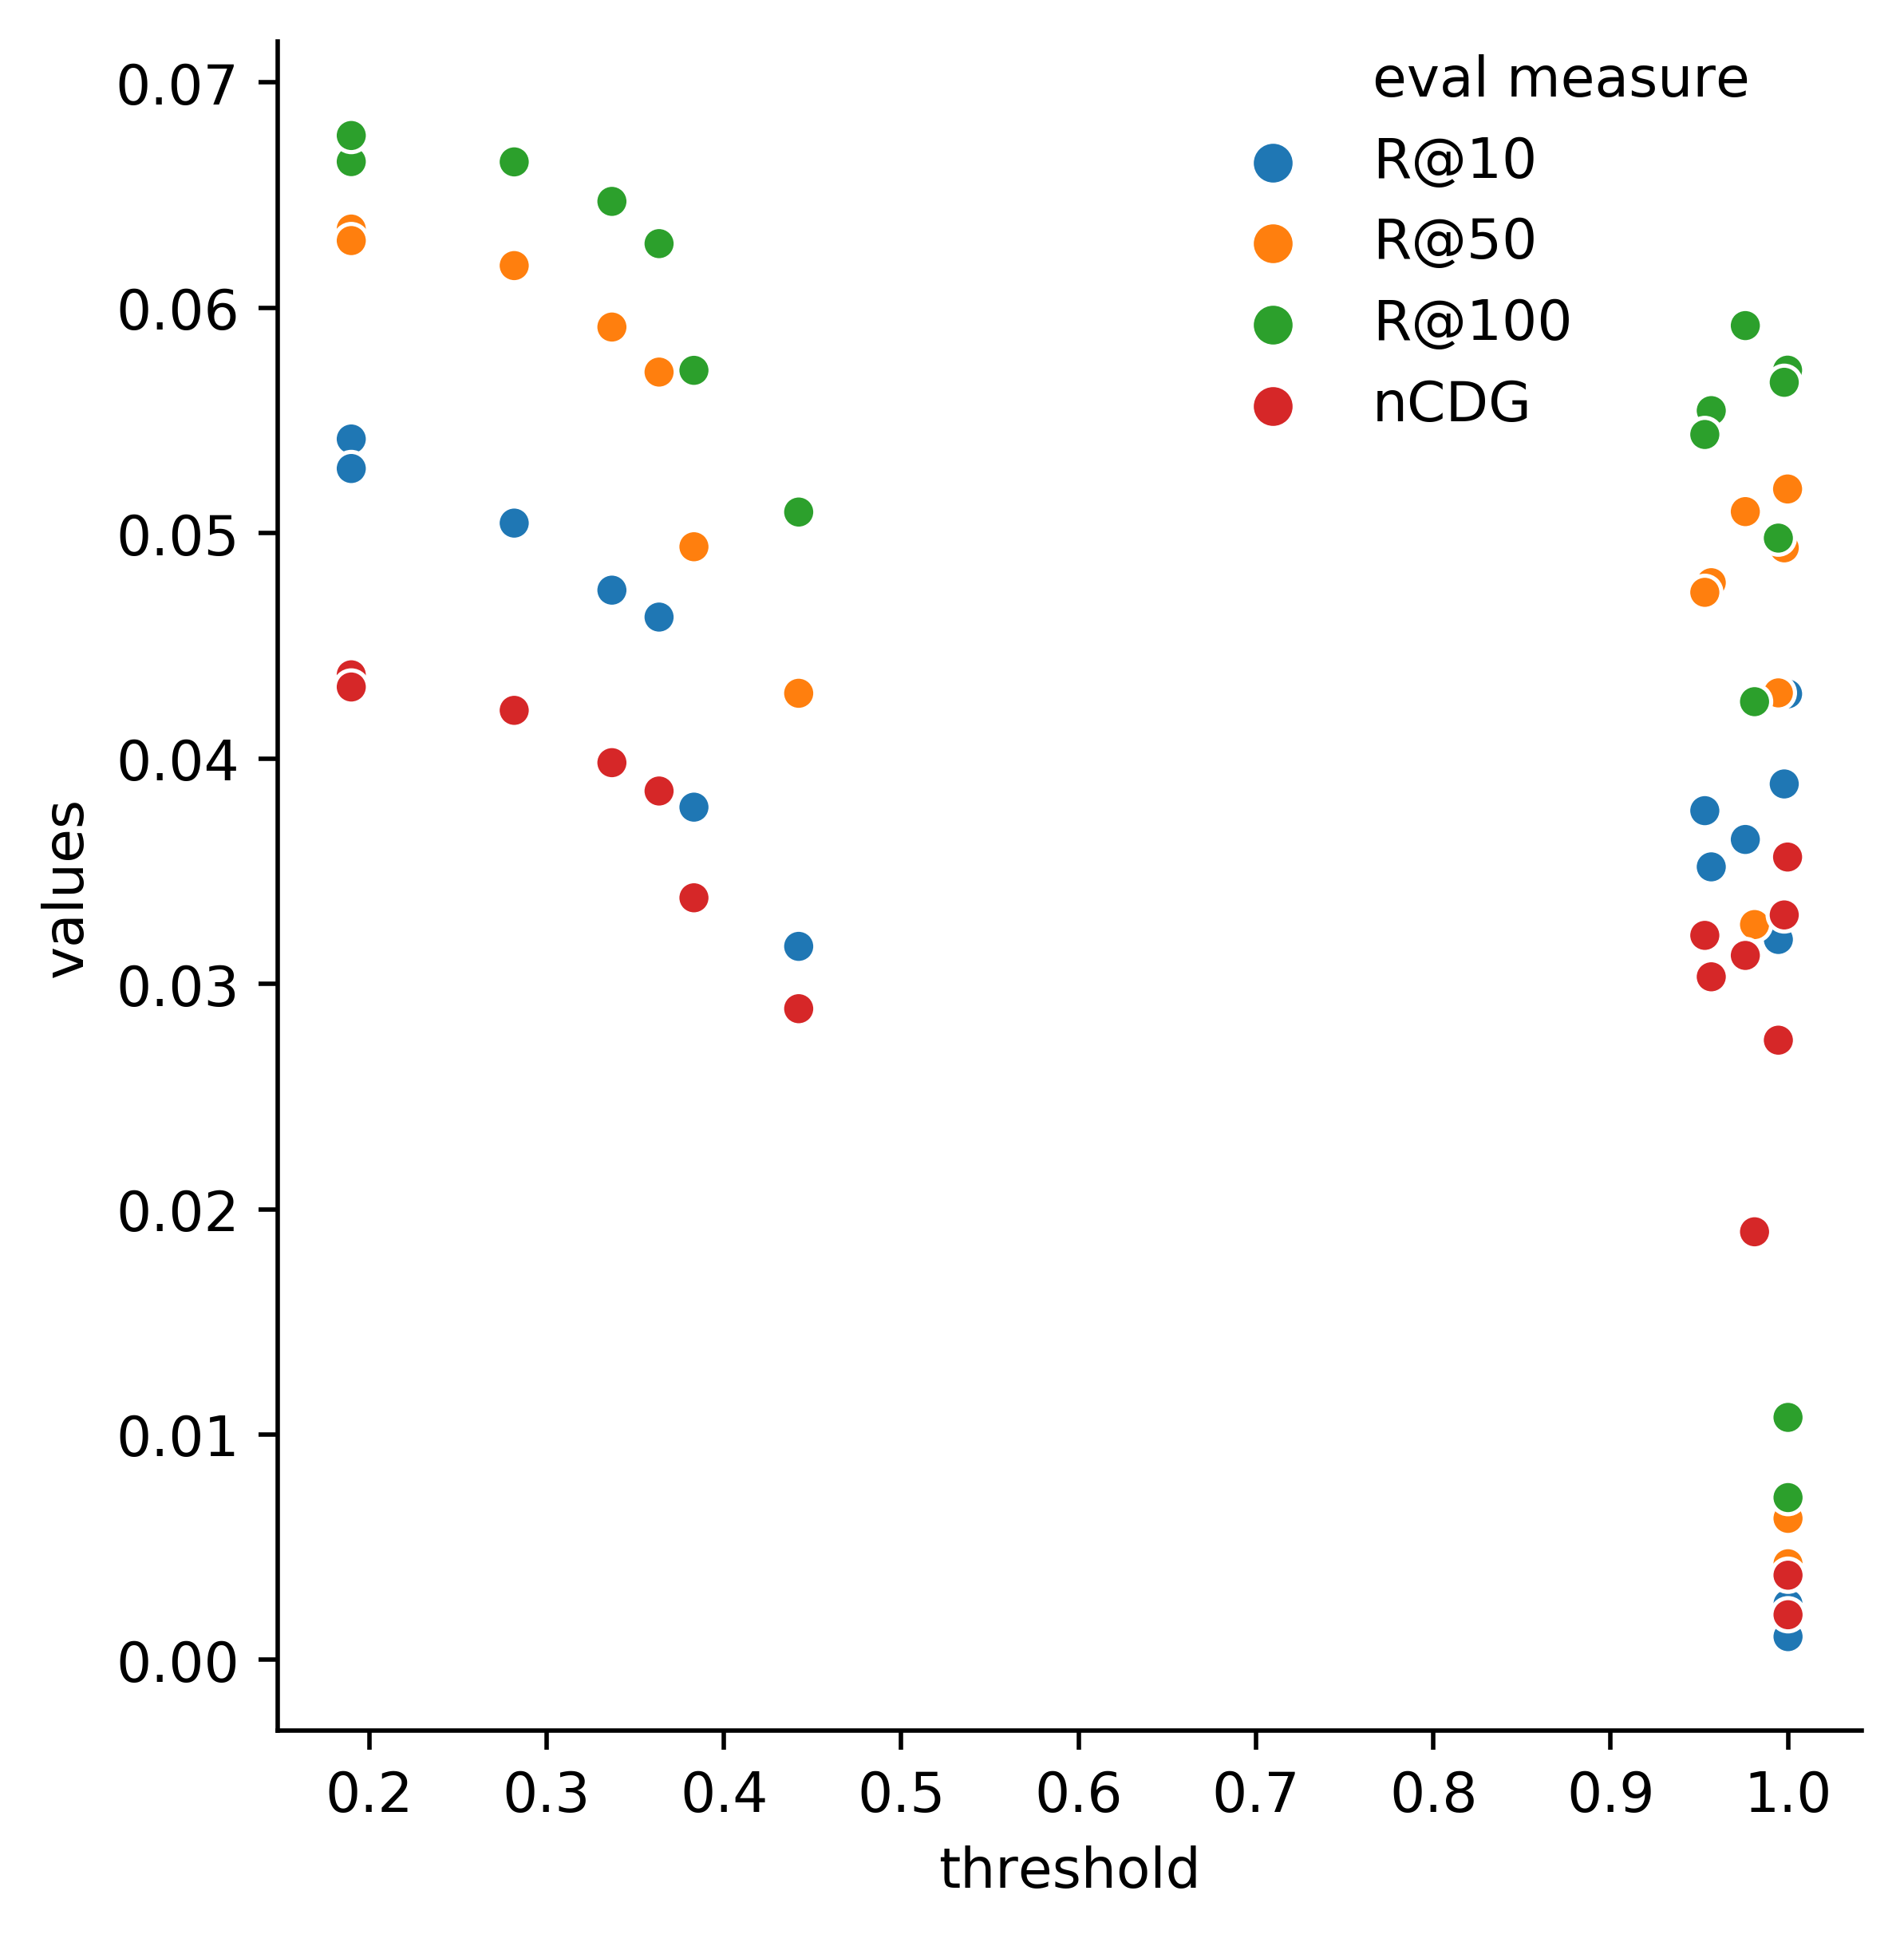
\includegraphics[width=1\linewidth]{./img/nn_threshold_performance_correlation.png}
	\caption[0.03\%-threshold value and performance correlation graph]{0.03\%-threshold value and performance correlation graph. \\ This graph visualized the correlation between the value of the threshold at position 846,700 in the $D_m$ of every method and the method's performances on various evaluation measures.}
	\label{fig:threshold_correlation_graph}
\end{figure}




